\documentclass[a4paper,11pt]{article}
\author{ 杨旭鹏  \  PB17000234}
\date{2019年秋季}
\title{计算物理A 第九题}

\usepackage{ctex}
\usepackage{amsmath}
\usepackage{amsfonts}
\usepackage{graphicx}
\usepackage{epstopdf}
\usepackage{lastpage}
\usepackage{hyperref}
\usepackage{listings}
\RequirePackage{xcolor}
\usepackage{appendix}
\usepackage{caption2}
\usepackage{subfigure}
\usepackage{float}
\makeatletter\def\@captype{table}\makeatother

\definecolor{dkgreen}{rgb}{0,0.6,0}
\definecolor{gray}{rgb}{0.5,0.5,0.5}
\definecolor{mauve}{rgb}{0.58,0,0.82}

\lstset{
  frame=tb,
  aboveskip=3mm,
  belowskip=3mm,
  showstringspaces=false,
  columns=flexible,
  framerule=1pt,
  rulecolor=\color{gray!35},
  backgroundcolor=\color{gray!5},
  basicstyle={\small\ttfamily},
  numbers=left,
  numberstyle=\tiny\color{gray},
  keywordstyle=\color{blue},
  commentstyle=\color{dkgreen},
  stringstyle=\color{mauve},
  breaklines=true,
  breakatwhitespace=true,
  tabsize=3,            
  }



\begin{document}
\maketitle

\section{题目描述}
自设若干个随机分布(相同或不同分布,它们有相同或不同的$\mu$和$\sigma$)通过Monte Carlo模拟,验证中心极限定理成立$(N =2,5,10)$。


\section{算法}
\subsection{中心极限定理}
设随机变量$x$满足概率密度分布函数$p(x)$,则对于任意$p(x)$都有:
\begin{equation}
\left\{
\begin{array}{l}
	p\left( \left |\frac{\left<x \right>-\mu}{\sigma/\sqrt{N}} \right| < \beta \right) \rightarrow \Phi(\beta) \\
	\left<x \right>  = \frac{1}{N}\sum_{i=1}^{N}x_{i} \\
	\mu = \int_{-\infty}^{\infty} xp(x)dx \\
	\sigma = \sqrt{E(x^{2})-(E(x))^{2}} = \sqrt{\int_{-\infty}^{\infty} x^{2}p(x)dx - \left( \int_{-\infty}^{\infty} xp(x)dx \right)^{2} }
\end{array}
\right.
\end{equation}
其中$\mu$为随机变量$x$的期望值,$\sigma$为$x$的标准差。则若想验证此条定理,可对满足某一分布的随机变量$x$进行$N$次抽样,计算统计量$\frac{\left<x \right>-\mu}{\sigma/\sqrt{N}} $,重复上述过程$n$次,则可得到对应抽样$N$次对应的统计量的近似概率分布($n$越大时此近似分布约接近该统计量的理论分布)。将得到的统计量的近似概率分布与标准正态分布比对,若当$n$越大时,两者越接近,即可验证此条定理。具体实现见代码。

\subsection{分布1}
设随机变量$x$满足概率分布:
\begin{equation}
p(x) = 
\left\{
\begin{array}{l}
x+1~~~~,if~x\in [-1,0]  \\
-x+1~~,if~x\in[0,1]  \\
0~~~~~~~~~~,otherwise	
\end{array}
\right.
\end{equation}

\begin{figure}[!htbp]        
\centering
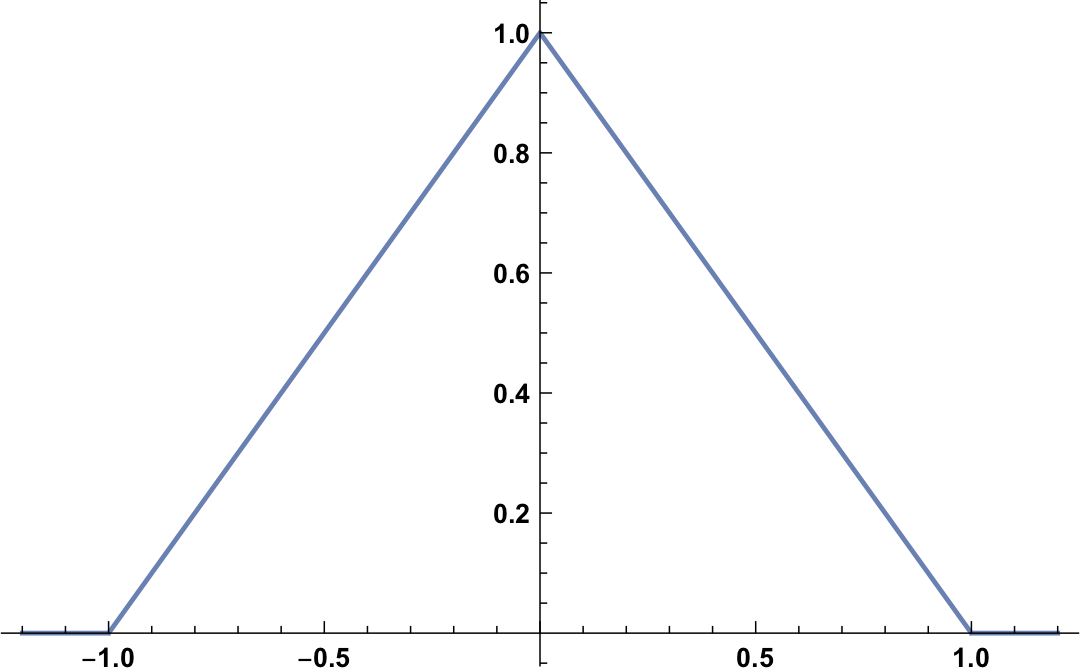
\includegraphics[width=10cm]{1.png}      
\caption{ 分布1的概率分布函数示意图}      
\end{figure}

则可得到其期望值和标准差为:$\mu = 0,\sigma = \frac{1}{\sqrt{6}}$,则按上述方法进行数值模拟即可。每次计算时所采取的抽样方法为直接抽样法:
\begin{equation}
\xi(x) = 
\left\{
\begin{array}{l}
\frac{x^{2}+1}{2}+x~~~~,if~x\in [-1,0]  \\
-\frac{x^{2}-1}{2}+x~~,if~x\in[0,1]  \\	
\end{array}
\right.
\end{equation}

其中$\xi(x)$为累积函数。容易求得其反函数:
\begin{equation}
x(\xi) = 
\left\{
\begin{array}{l}
\sqrt{2\xi}-1~~~~,if~\xi\in [0,0.5]  \\
1-\sqrt{2(1-\xi)}~~,if~\xi\in[0.5,1]  \\	
\end{array}
\right.
\end{equation}

$\xi$可在$[0,1]$区间内均匀抽取得到,即可进行直接抽样。



\subsection{分布2}
设随机变量$x$满足概率分布:
\begin{equation}
p(x) = 
\left\{
\begin{array}{l}
1~~~~,if~x\in [1,2]  \\
0~~~~,otherwise	
\end{array}
\right.
\end{equation}

\begin{figure}[!htbp]        
\centering
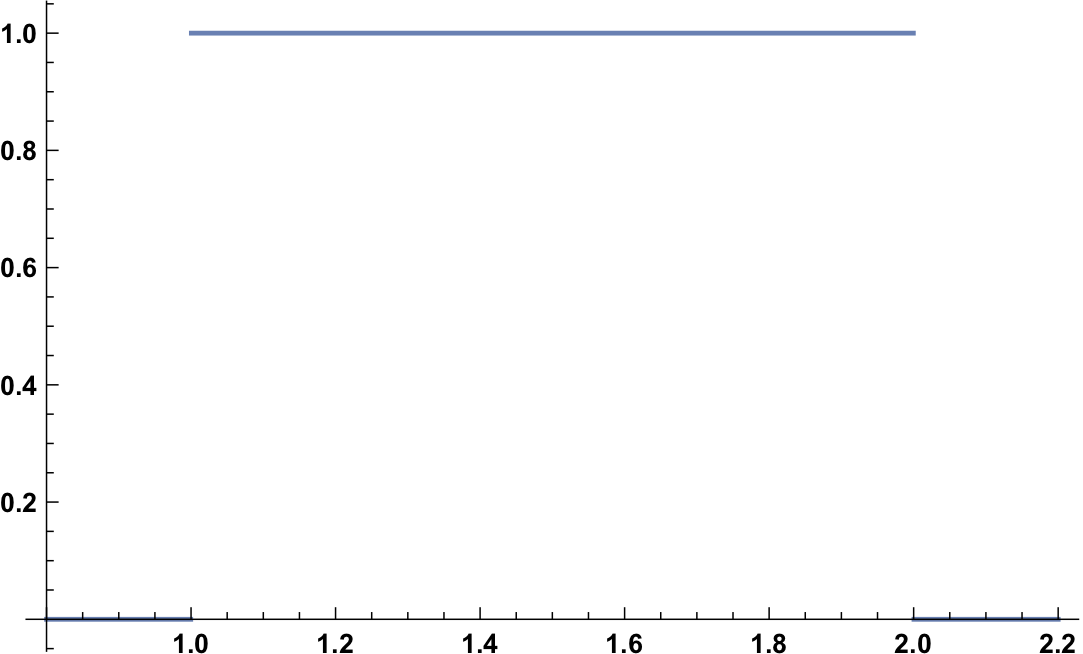
\includegraphics[width=10cm]{2.png}      
\caption{ 分布2的概率分布函数示意图}      
\end{figure}

则可得到其期望值和标准差为:$\mu = 0.5,\sigma = \frac{1}{\sqrt{12}}$,则按上述方法进行数值模拟即可。其每次计算时的抽样可利用$[0,1]$区间内均与分布的抽样点向正方向平移1得到。

\subsection{分布3}
设随机变量$x$满足概率分布:
\begin{equation}
p(x) = 
\left\{
\begin{array}{l}
x+1~~~~,if~x\in [-1,0]  \\
0.5~~~~~,if~x\in[0,1]  \\
0~~~~~~~~~~,otherwise	
\end{array}
\right.
\end{equation}

\begin{figure}[!htbp]        
\centering
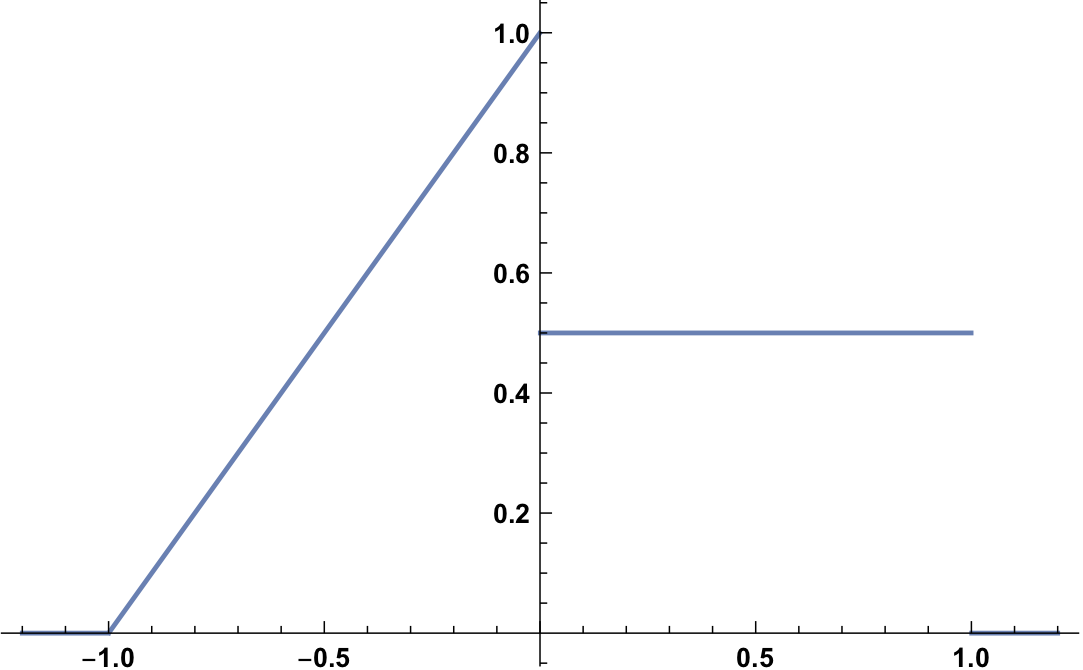
\includegraphics[width=10cm]{3.png}      
\caption{ 分布3的概率分布函数示意图}      
\end{figure}

则可得到其期望值和标准差为:$\mu = \frac{1}{12} ,\sigma = \frac{\sqrt{35}}{12}$,则按上述方法进行数值模拟即可。每次计算时所采取的抽样方法为直接抽样法:
\begin{equation}
\xi(x) = 
\left\{
\begin{array}{l}
\frac{x^{2}+1}{2}+x~~~~,if~x\in [-1,0]  \\
\frac{x+1}{2}~~~~~,if~x\in[0,1]  \\	
\end{array}
\right.
\end{equation}
其中$\xi(x)$为累积函数。容易求得其反函数:
\begin{equation}
x(\xi) = 
\left\{
\begin{array}{l}
\sqrt{2\xi}-1~~~~,if~\xi\in [0,0.5]  \\
2\xi-1~~~~~,if~\xi\in[0.5,1]  \\	
\end{array}
\right.
\end{equation}
其中$\xi$可在$[0,1]$区间内均匀抽取得到,即可进行直接抽样。





\subsection{16807产生器}
16807产生器属于线性同余法产生器的特例。而线性同余法方法为:

\begin{equation}
\begin{aligned}
	I_{n+1} &= (aI_{n} + b) \ mod \ m \\
	x_{n} &= I_{n}/m
\end{aligned}
\label{linear}	
\end{equation}

其中整数$I_{i} \in [0,m-1]$,$a,b,m$为算法中的可调参数,其选取直接影响产生器的质量。选取参数:
\begin{equation}
\left\{
\begin{array}{l}
	a = 7^{5} = 16807 \\
	b = 0 \\
	m = 2^{31}-1 = 2147483647
\end{array}
\right.
\end{equation}

即为所谓的16807产生器。由于直接利用\ref{linear}编写程序时计算$(aI_{n} \ mod \ m )$时很容易造成数据溢出,故采取Schrage方法进行具体编程的实现:

\begin{equation}
	aI_{n} \ mod \ m = \left\{
	\begin{array}{l}
		a(I_{n}\ mod \ q) - r[I_{n}/q],\ \ \ \ \ \ \ \ if \geq 0 \\
		a(I_{n}\ mod \ q) - r[I_{n}/q] + m,\ \ otherwise	
			\end{array}
	\right.
\end{equation}

其中$m=aq+r$,即$q=m/a=127773$,$r=m \ mod \ a=2836$。即可利用此方法产生伪随机数序列。



\section{程序使用方法}
在运行程序后,会看到请求输入所需计算的统计量个数的提示,按照提示在后面输入所需要的总计算次数,摁回车继续。屏幕请求输入每次计算统计量所用的点数,输入后摁回车继续。然后经过计算统计出3个分布在$[-3,3]$上剖分的$o$个小区间上计算的统计量出现的概率到数据文件。\footnote{$o$可在程序宏定义中更改,默认值为600,即每个小区间长度为0.01}程序输出完这些后会自动退出。

\begin{figure}[!htbp]        
\centering

\includegraphics[width=7cm]{example.png}      
\caption{ 一个典型程序的运行示例}      
\end{figure}


\section{程序结果与讨论}
当输入一些不同的计算次数时,得到如下结果\footnote{以下的结果是将$[-3,3]$剖分为600个小区间得到的(即每个小区间的长度为$0.01$)其中概率为在$[-3,3]$之间归一化后的结果,例如对于在$[x_{i},x_{i+1}]$中出现的概率,对于抽样点来说即为:$p_{i} = \frac{n_{i}}{N}$($n_{i}$为统计量落在此区间内的个数,$N$为计算总次数数);对于理论频率(标准正态分布)来说,即为:$p_{i} = \frac{ \int_{x_{i}}^{x_{i+1}}p(x)dx }{ \int_{-3}^{3}p(x)dx } \doteq \frac{ p(\frac{x_{2}+x_{i+1}}{2})\Delta x }{ \int_{-3}^{3}p(x)dx }$(其中$\Delta x$为区间长度,$p(x)$为标准正态分布的密度函数)}:


\begin{figure}[!htbp]   
\centering     
\subfigure[每次抽样2个点]{
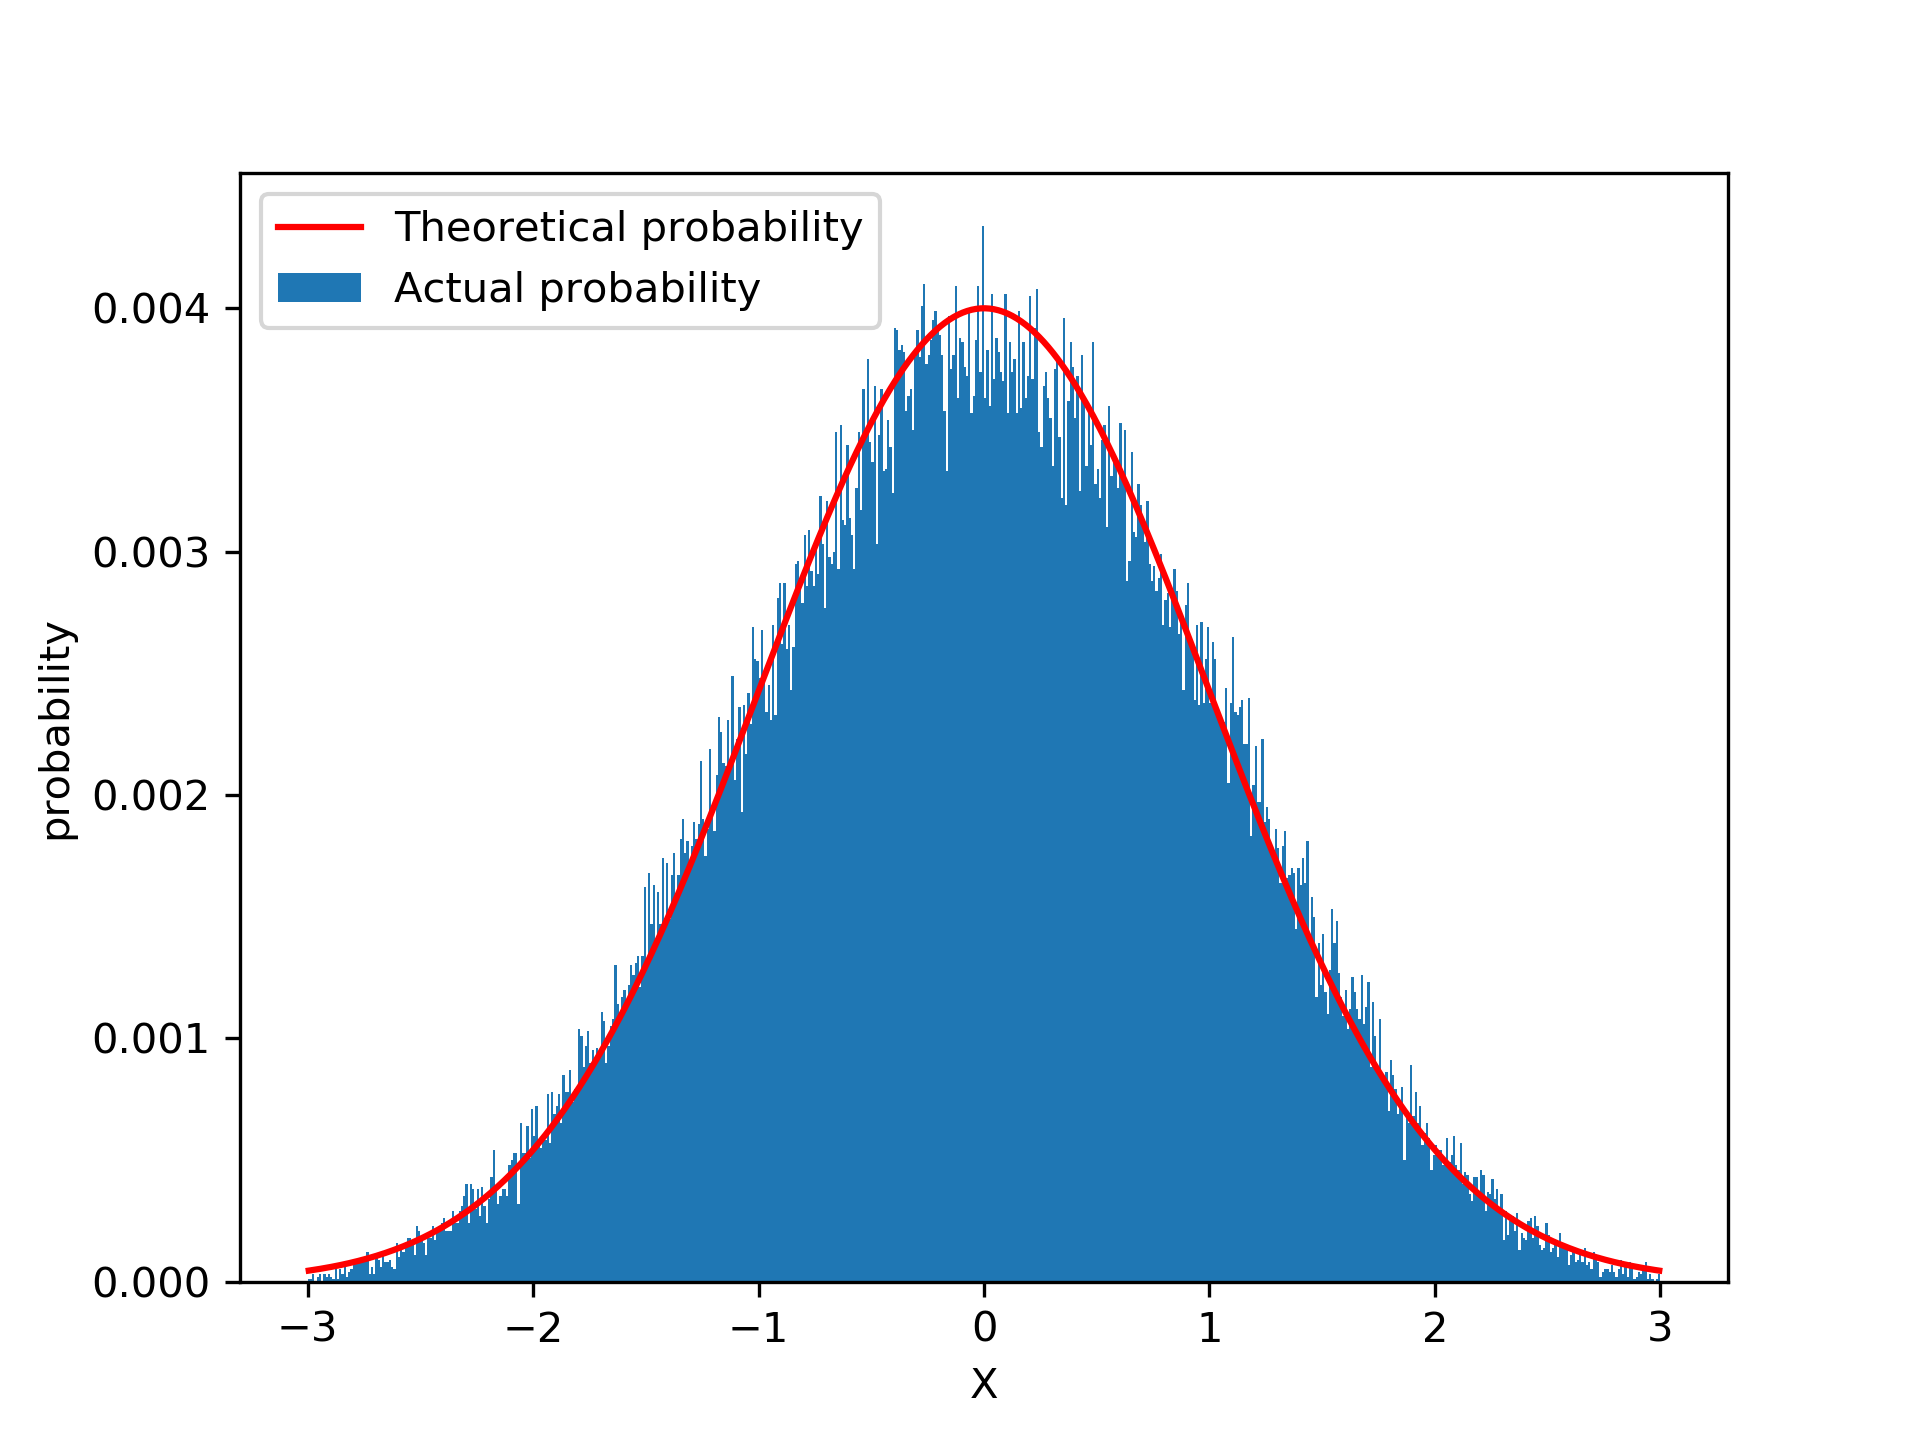
\includegraphics[width=4cm] {1-5-2.png}
}
\subfigure[每次抽样5个点]{
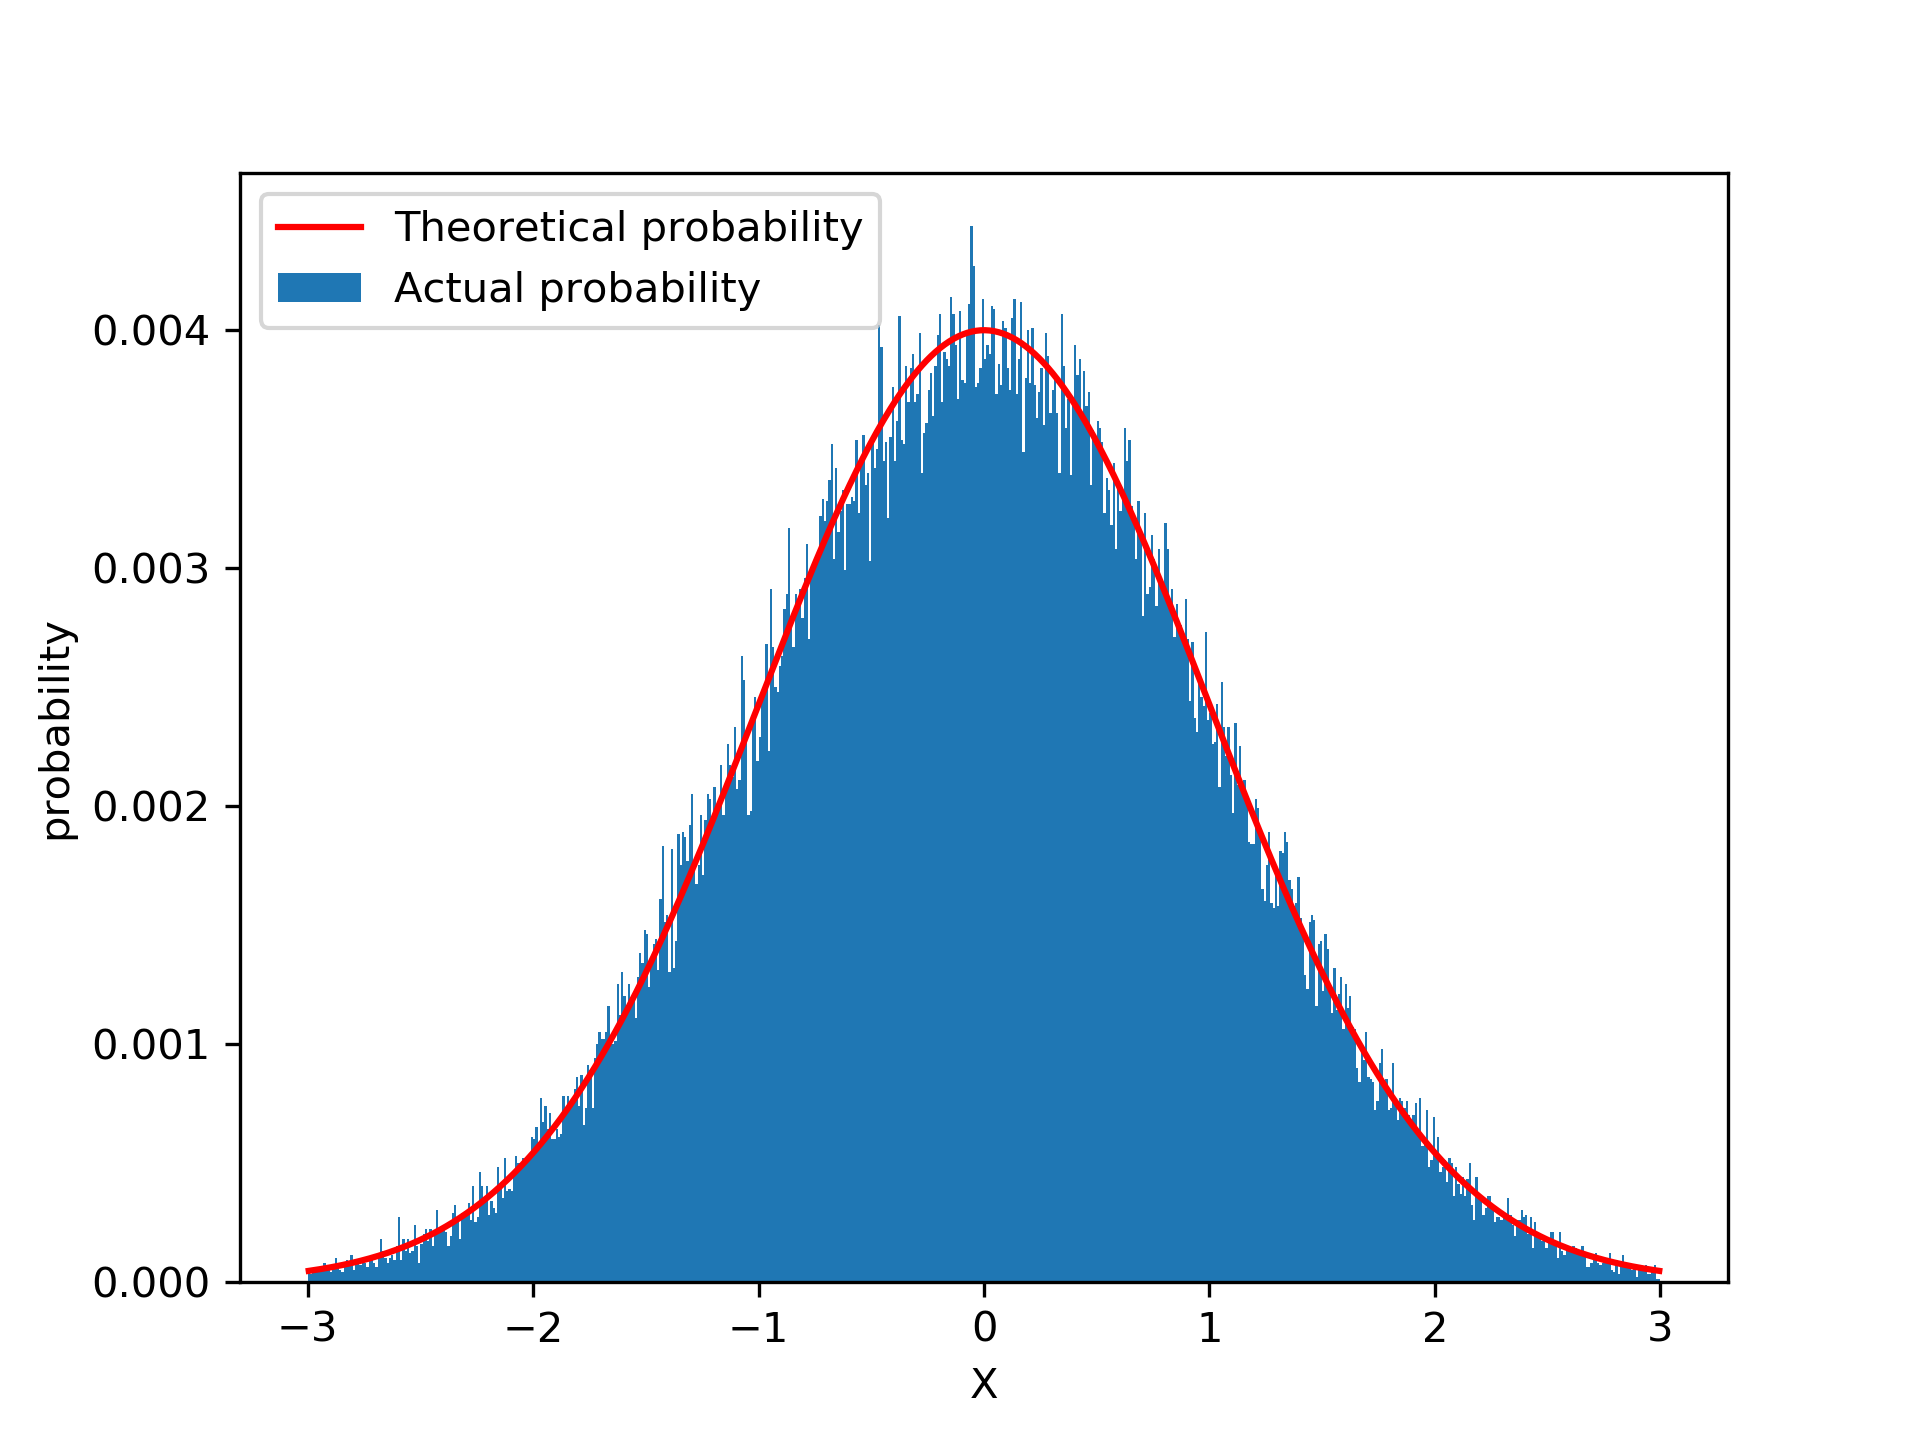
\includegraphics[width=4cm] {1-5-5.png}
}      
\subfigure[每次抽样10个点]{
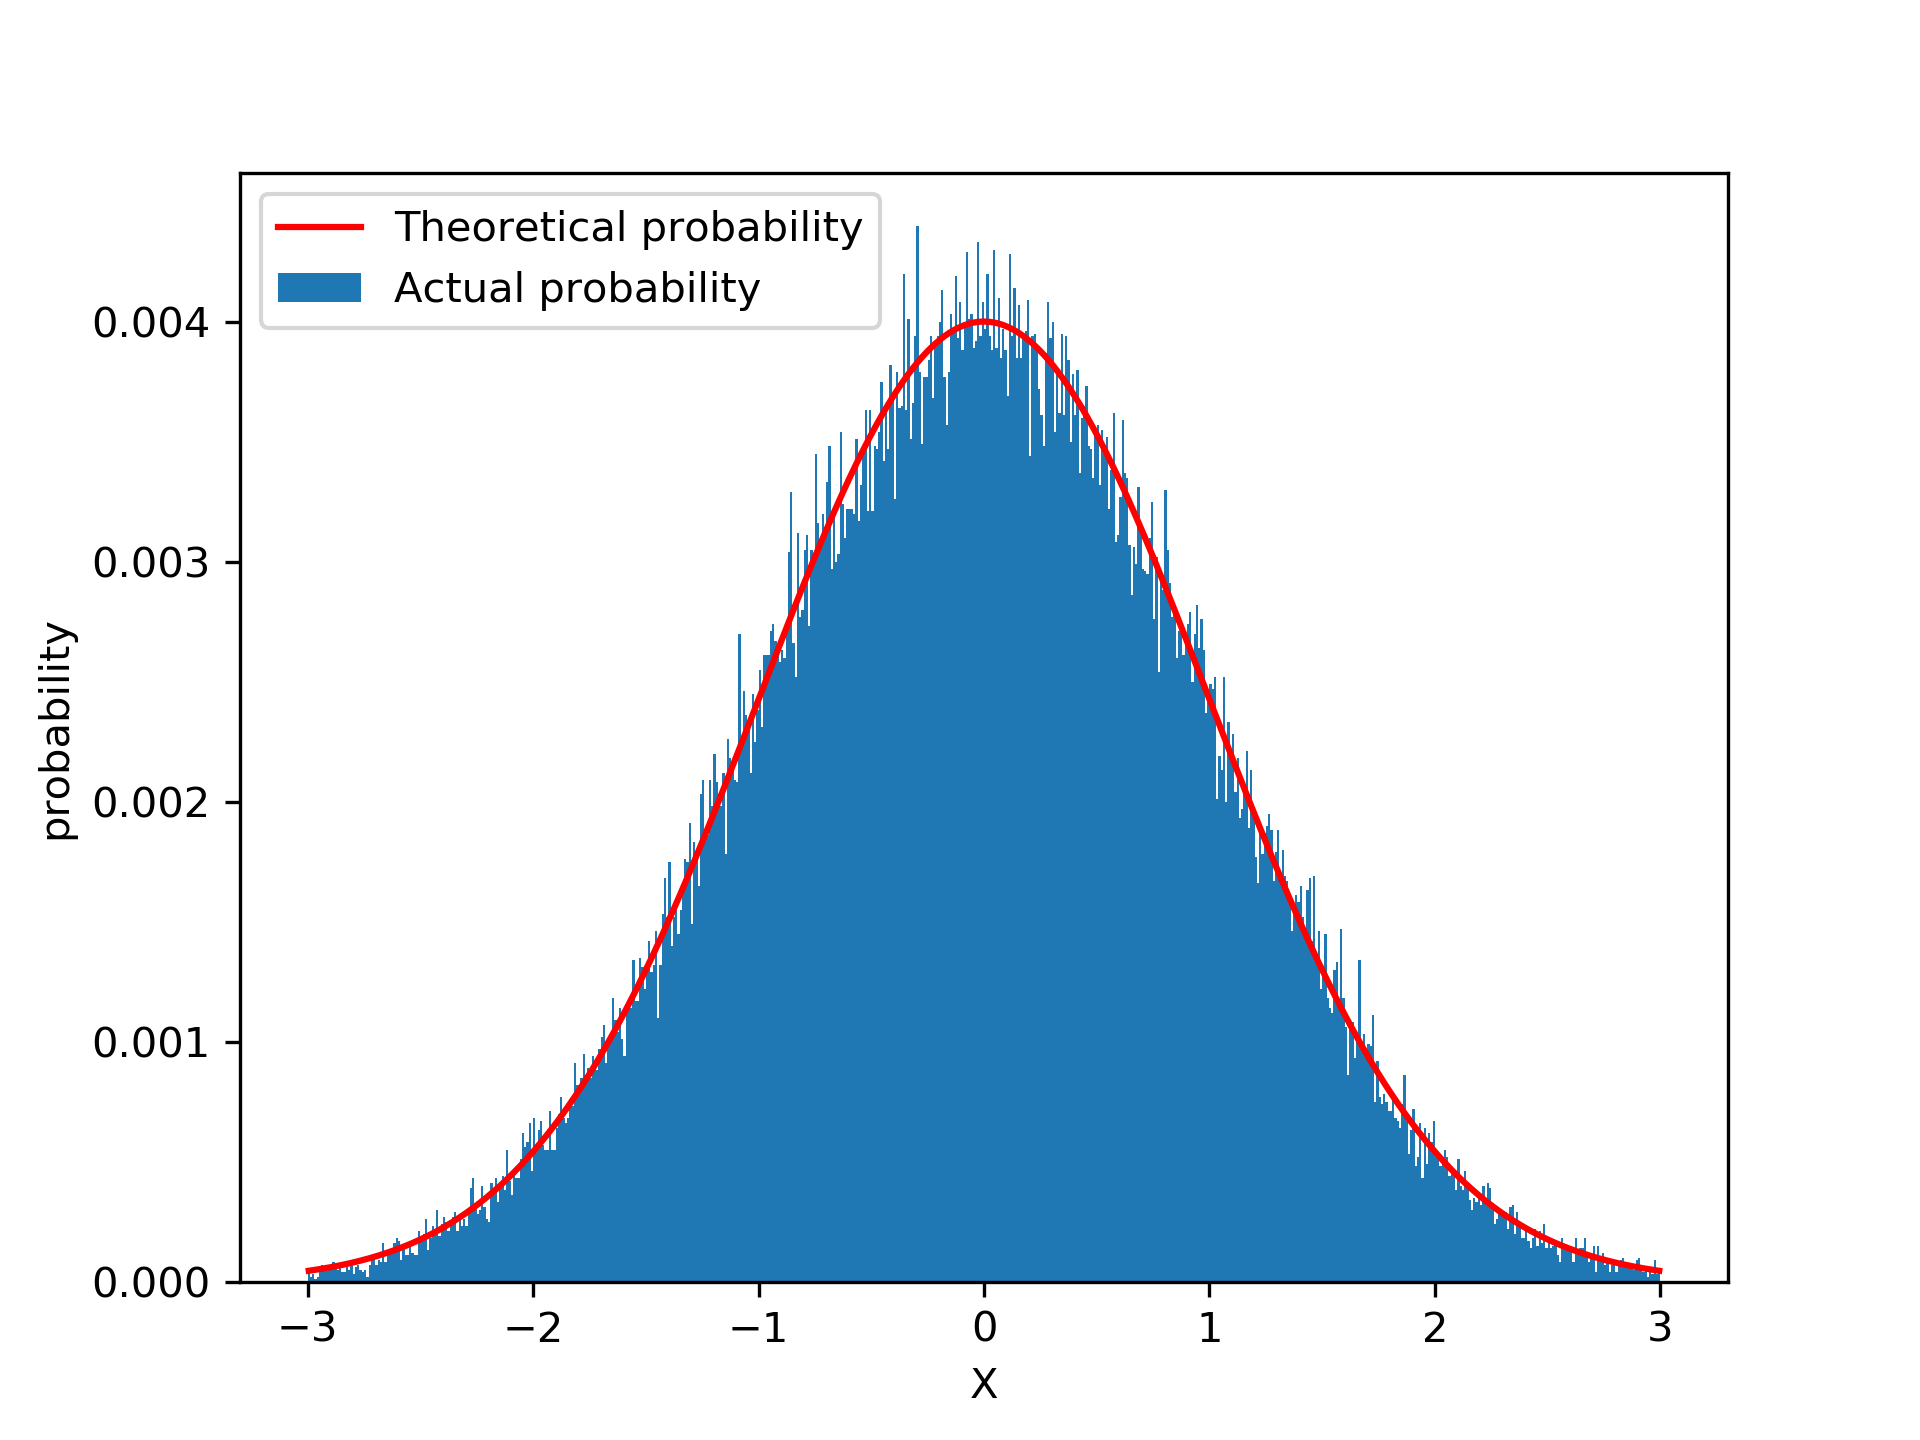
\includegraphics[width=4cm] {1-5-10.png}
}      
\caption{1号分布计算$10^{5}$次后的结果}      
\end{figure}


\begin{figure}[!htbp]   
\centering     
\subfigure[每次抽样2个点]{
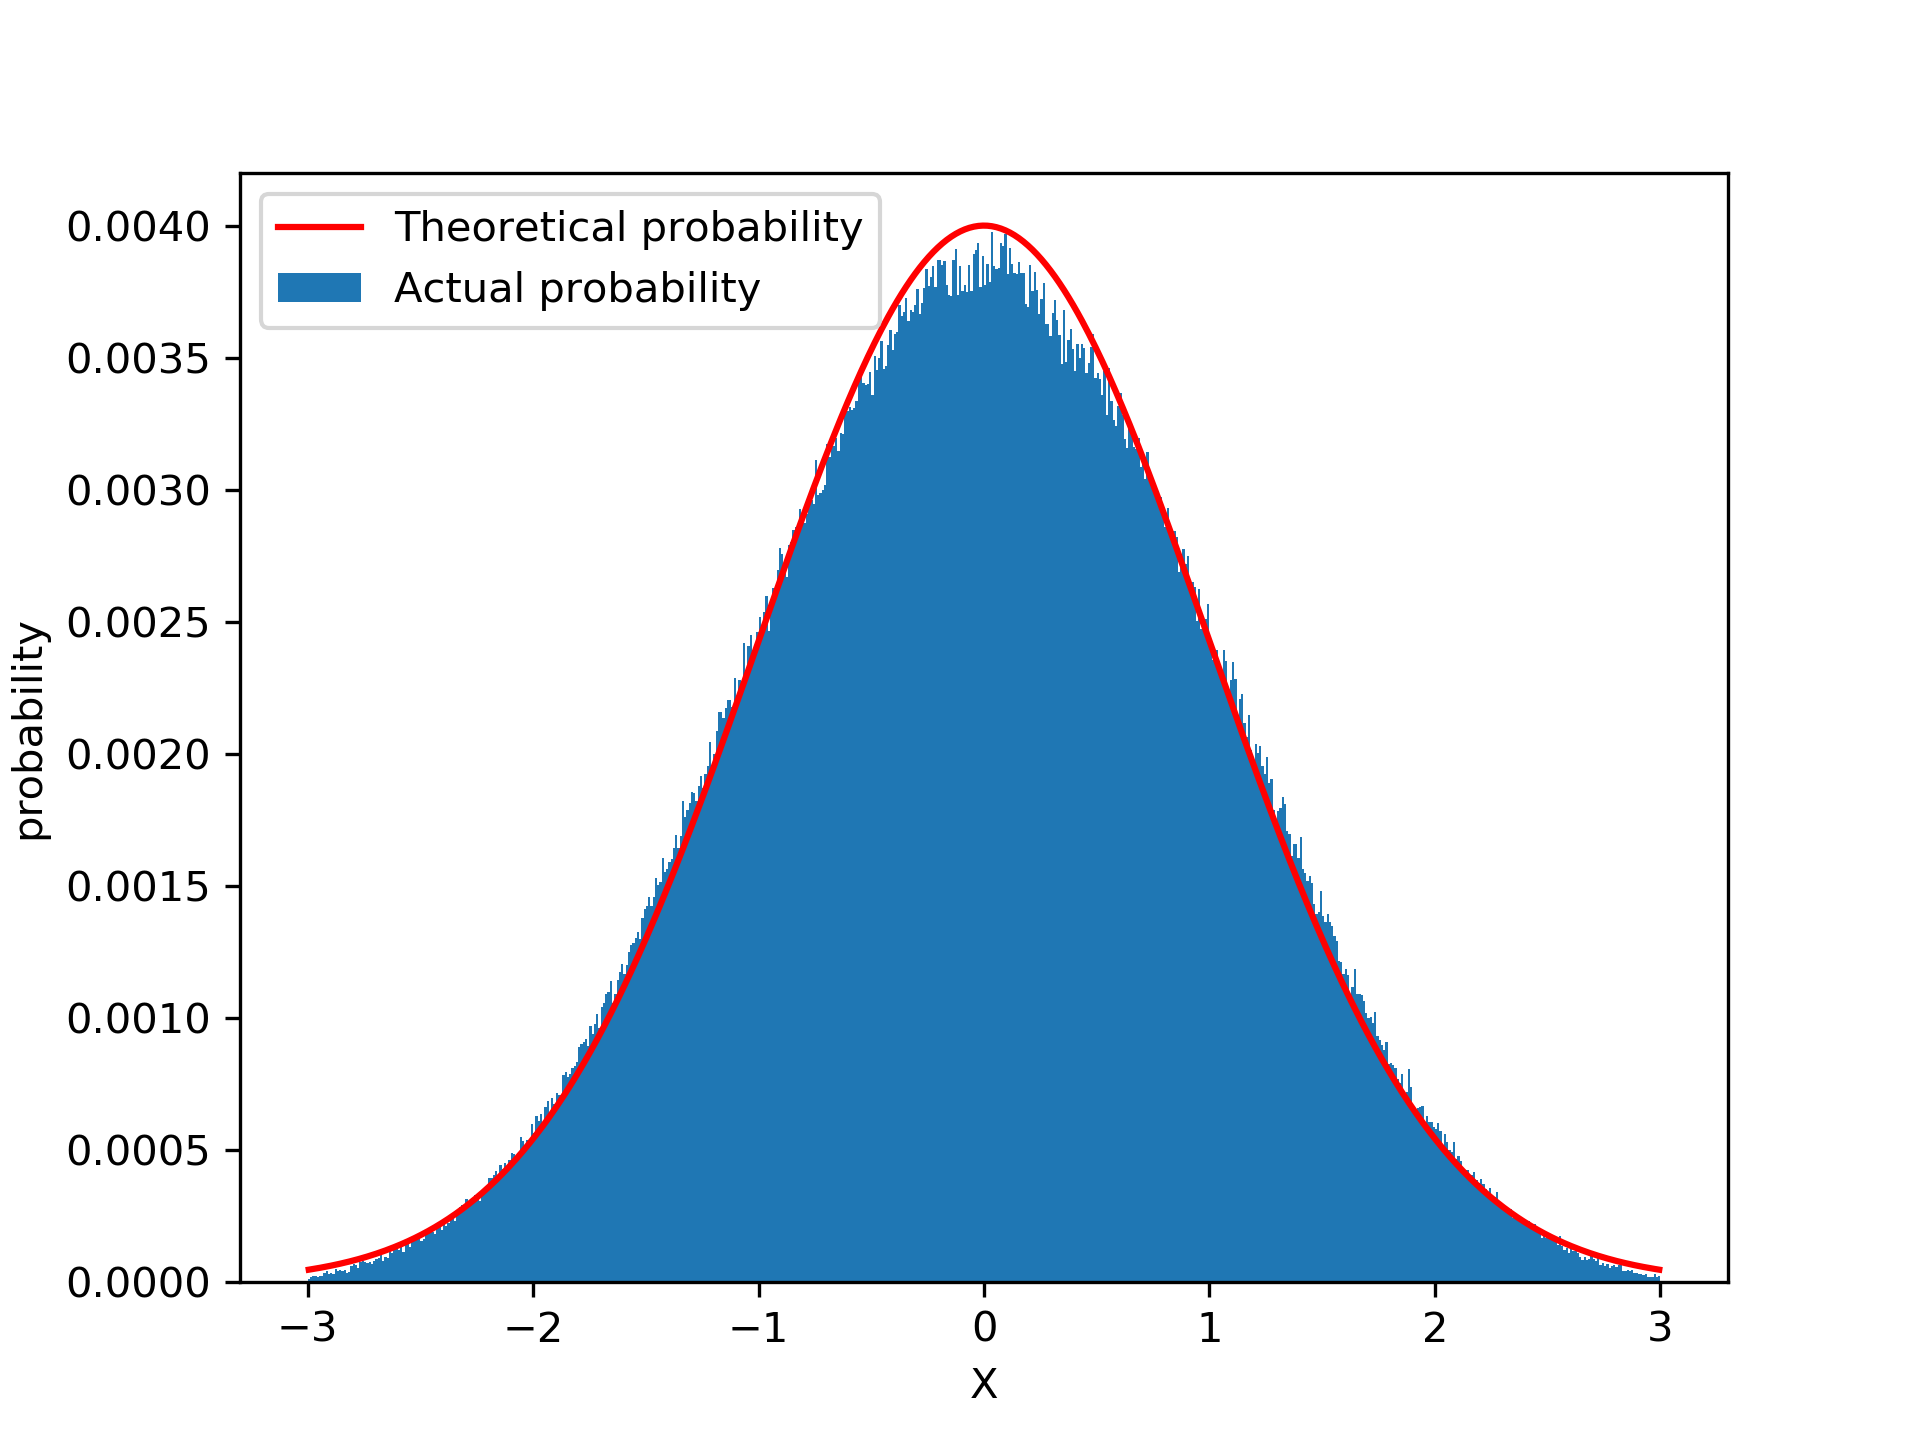
\includegraphics[width=4cm] {1-6-2.png}
}
\subfigure[每次抽样5个点]{
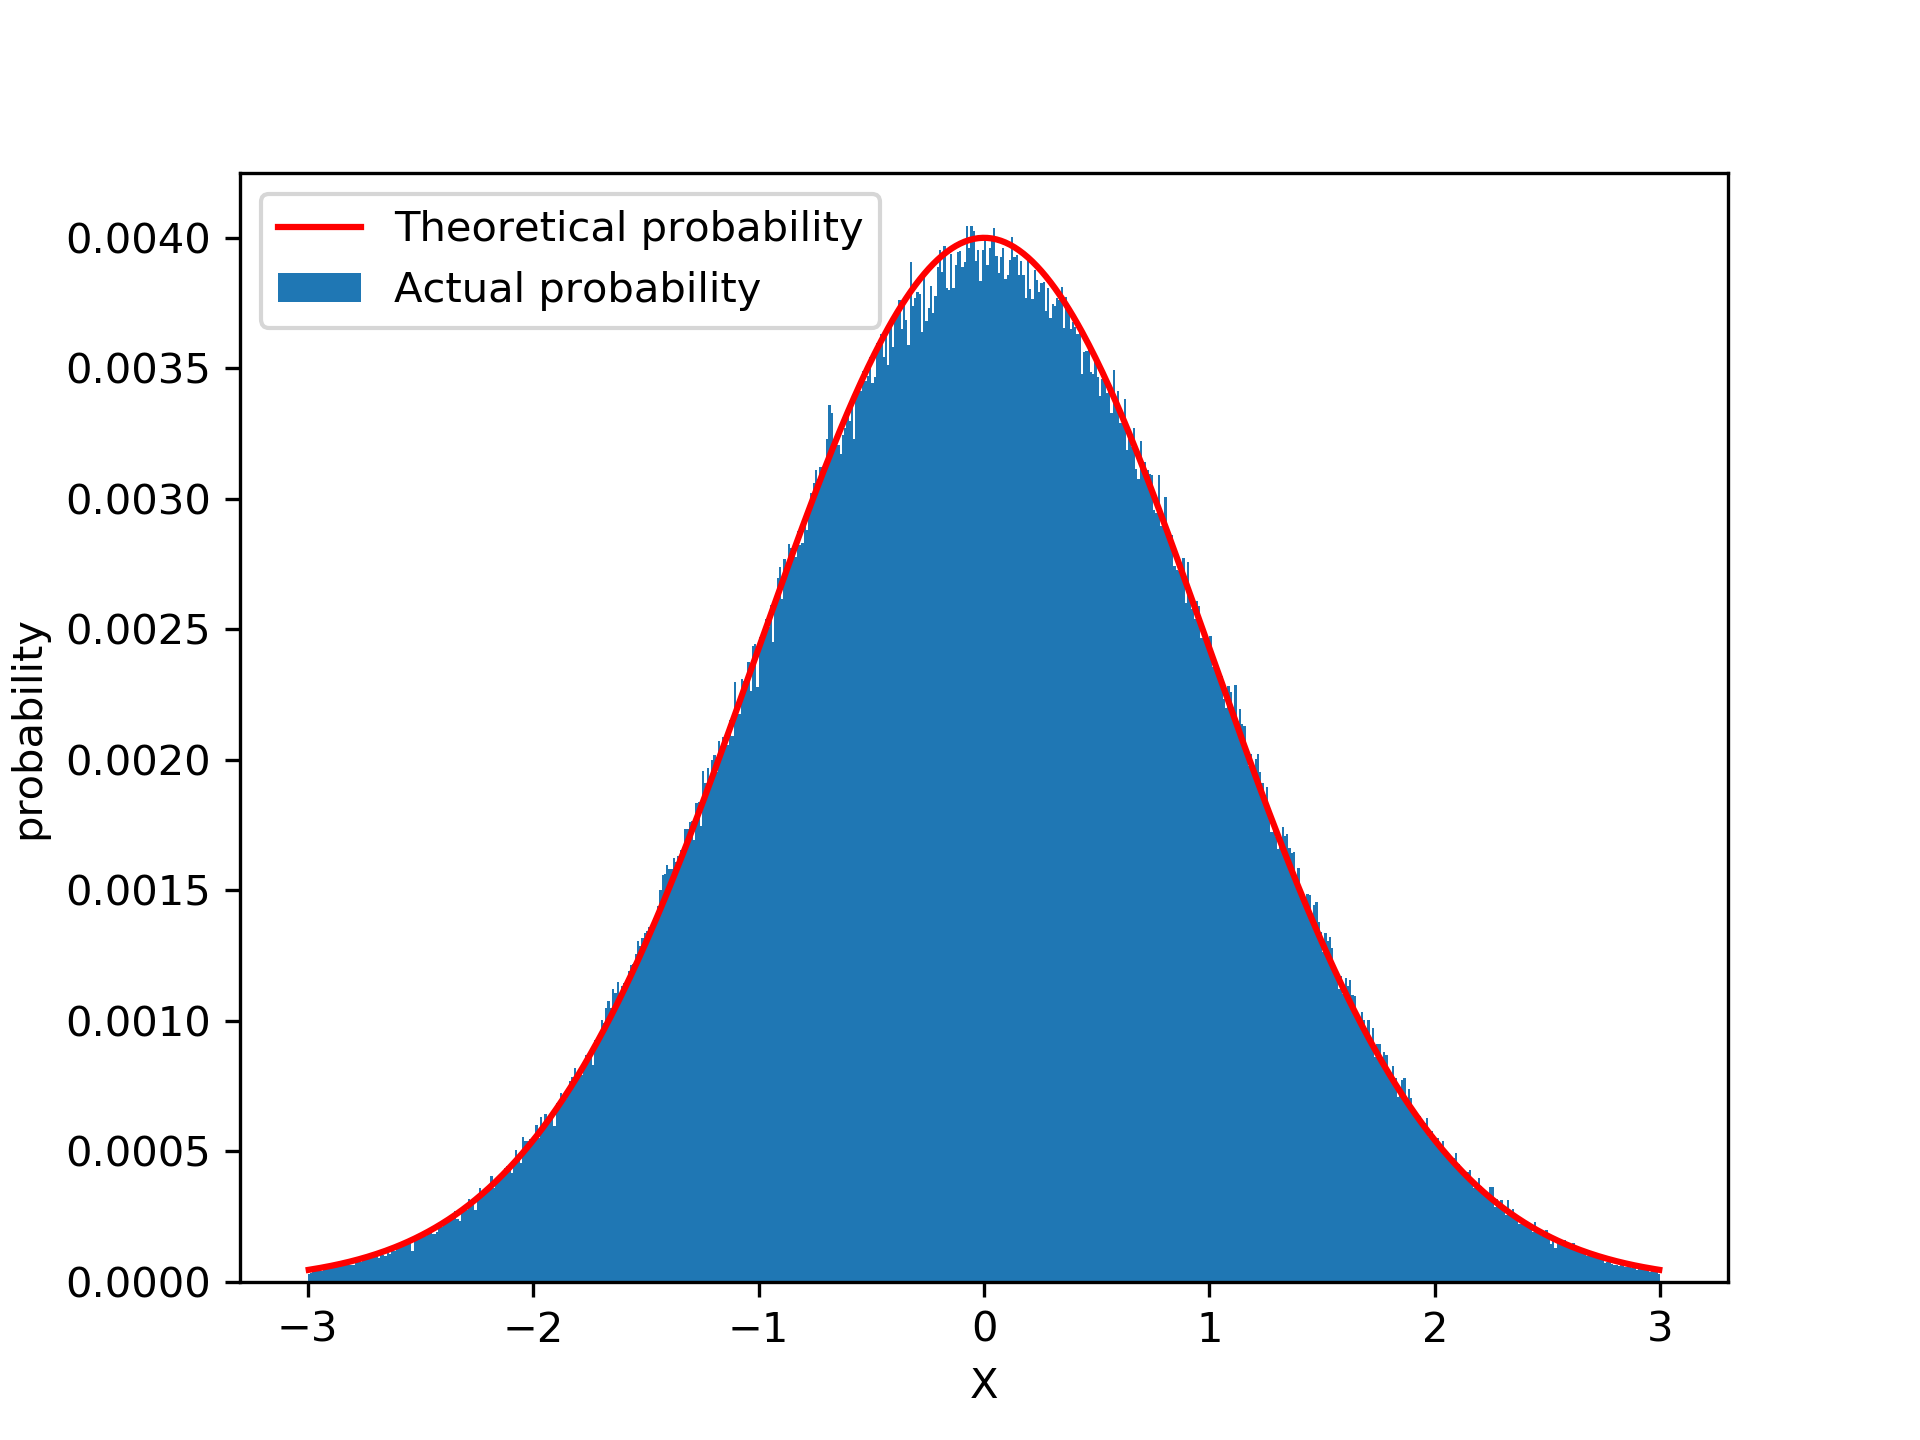
\includegraphics[width=4cm] {1-6-5.png}
}      
\subfigure[每次抽样10个点]{
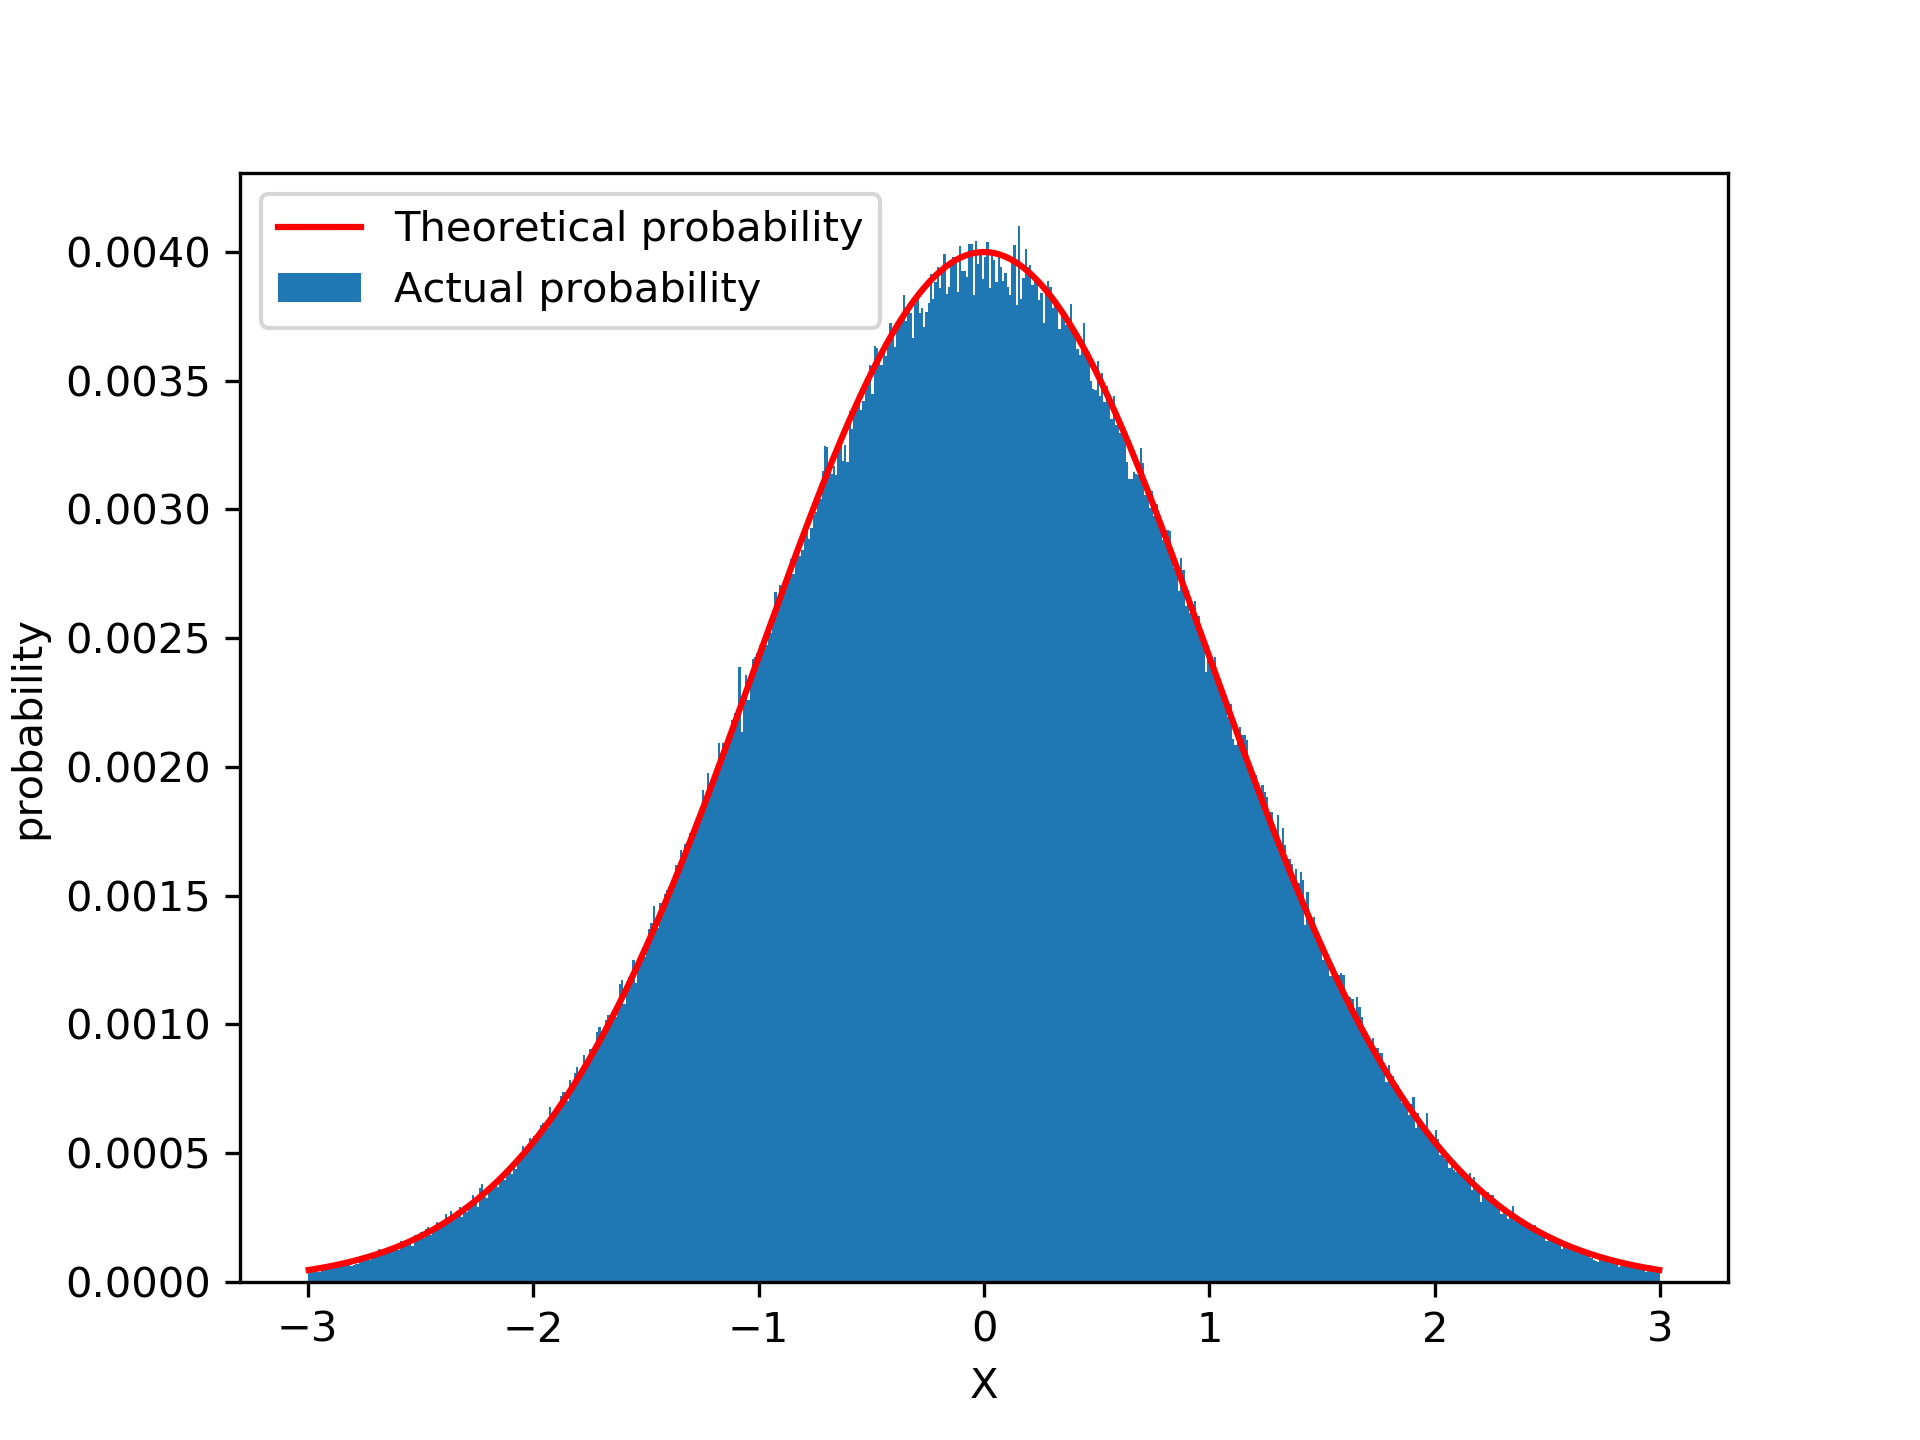
\includegraphics[width=4cm] {1-6-10.png}
}      
\caption{1号分布计算$10^{6}$次后的结果}      
\end{figure}


\begin{figure}[!htbp]   
\centering     
\subfigure[每次抽样2个点]{
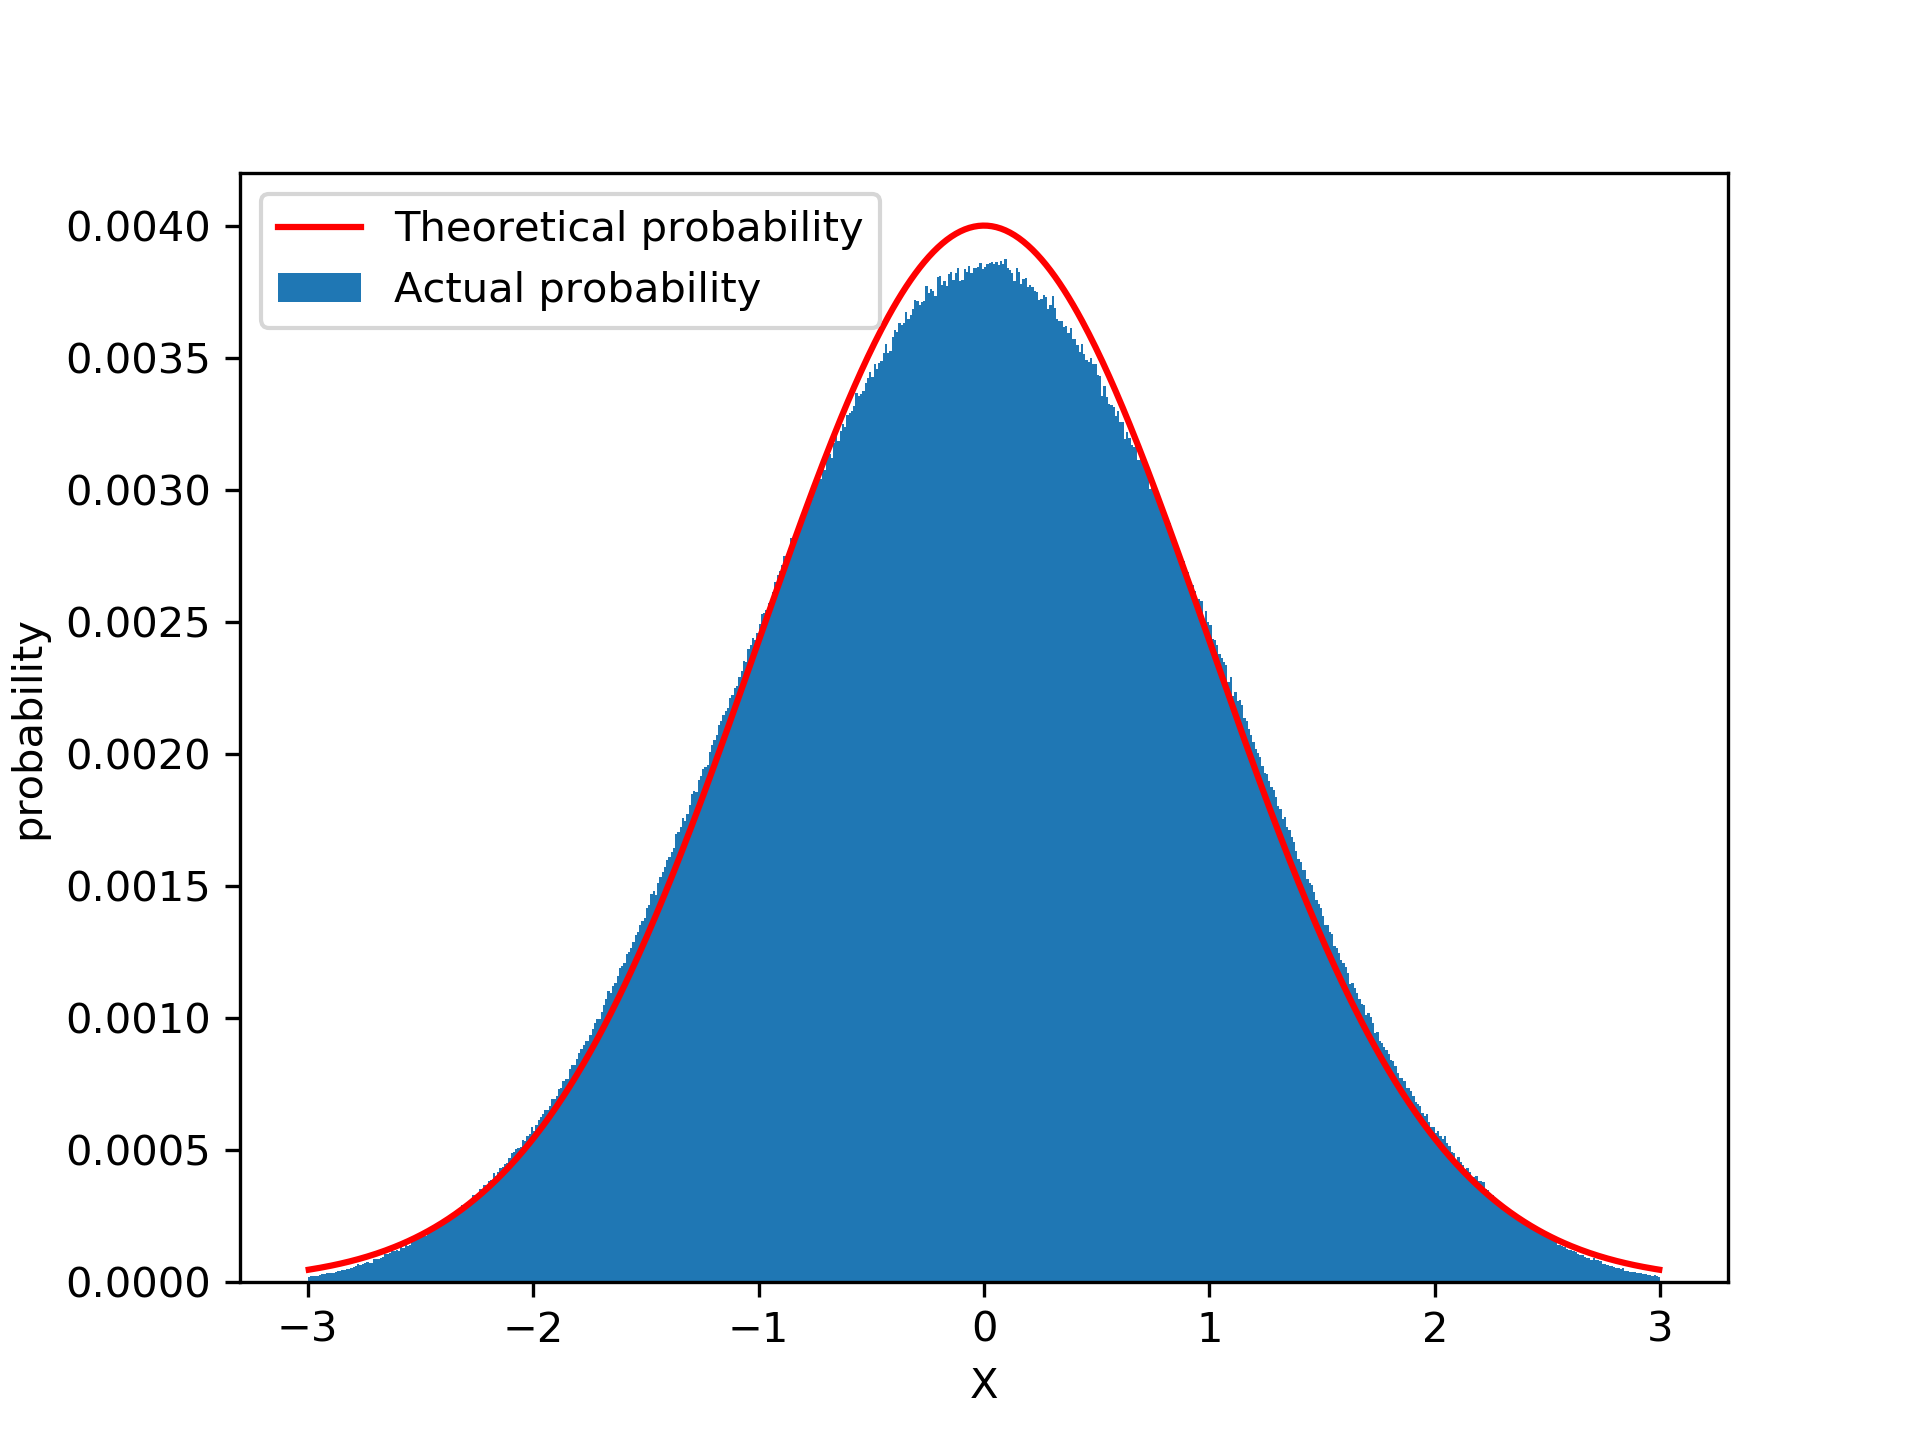
\includegraphics[width=4cm] {1-7-2.png}
}
\subfigure[每次抽样5个点]{
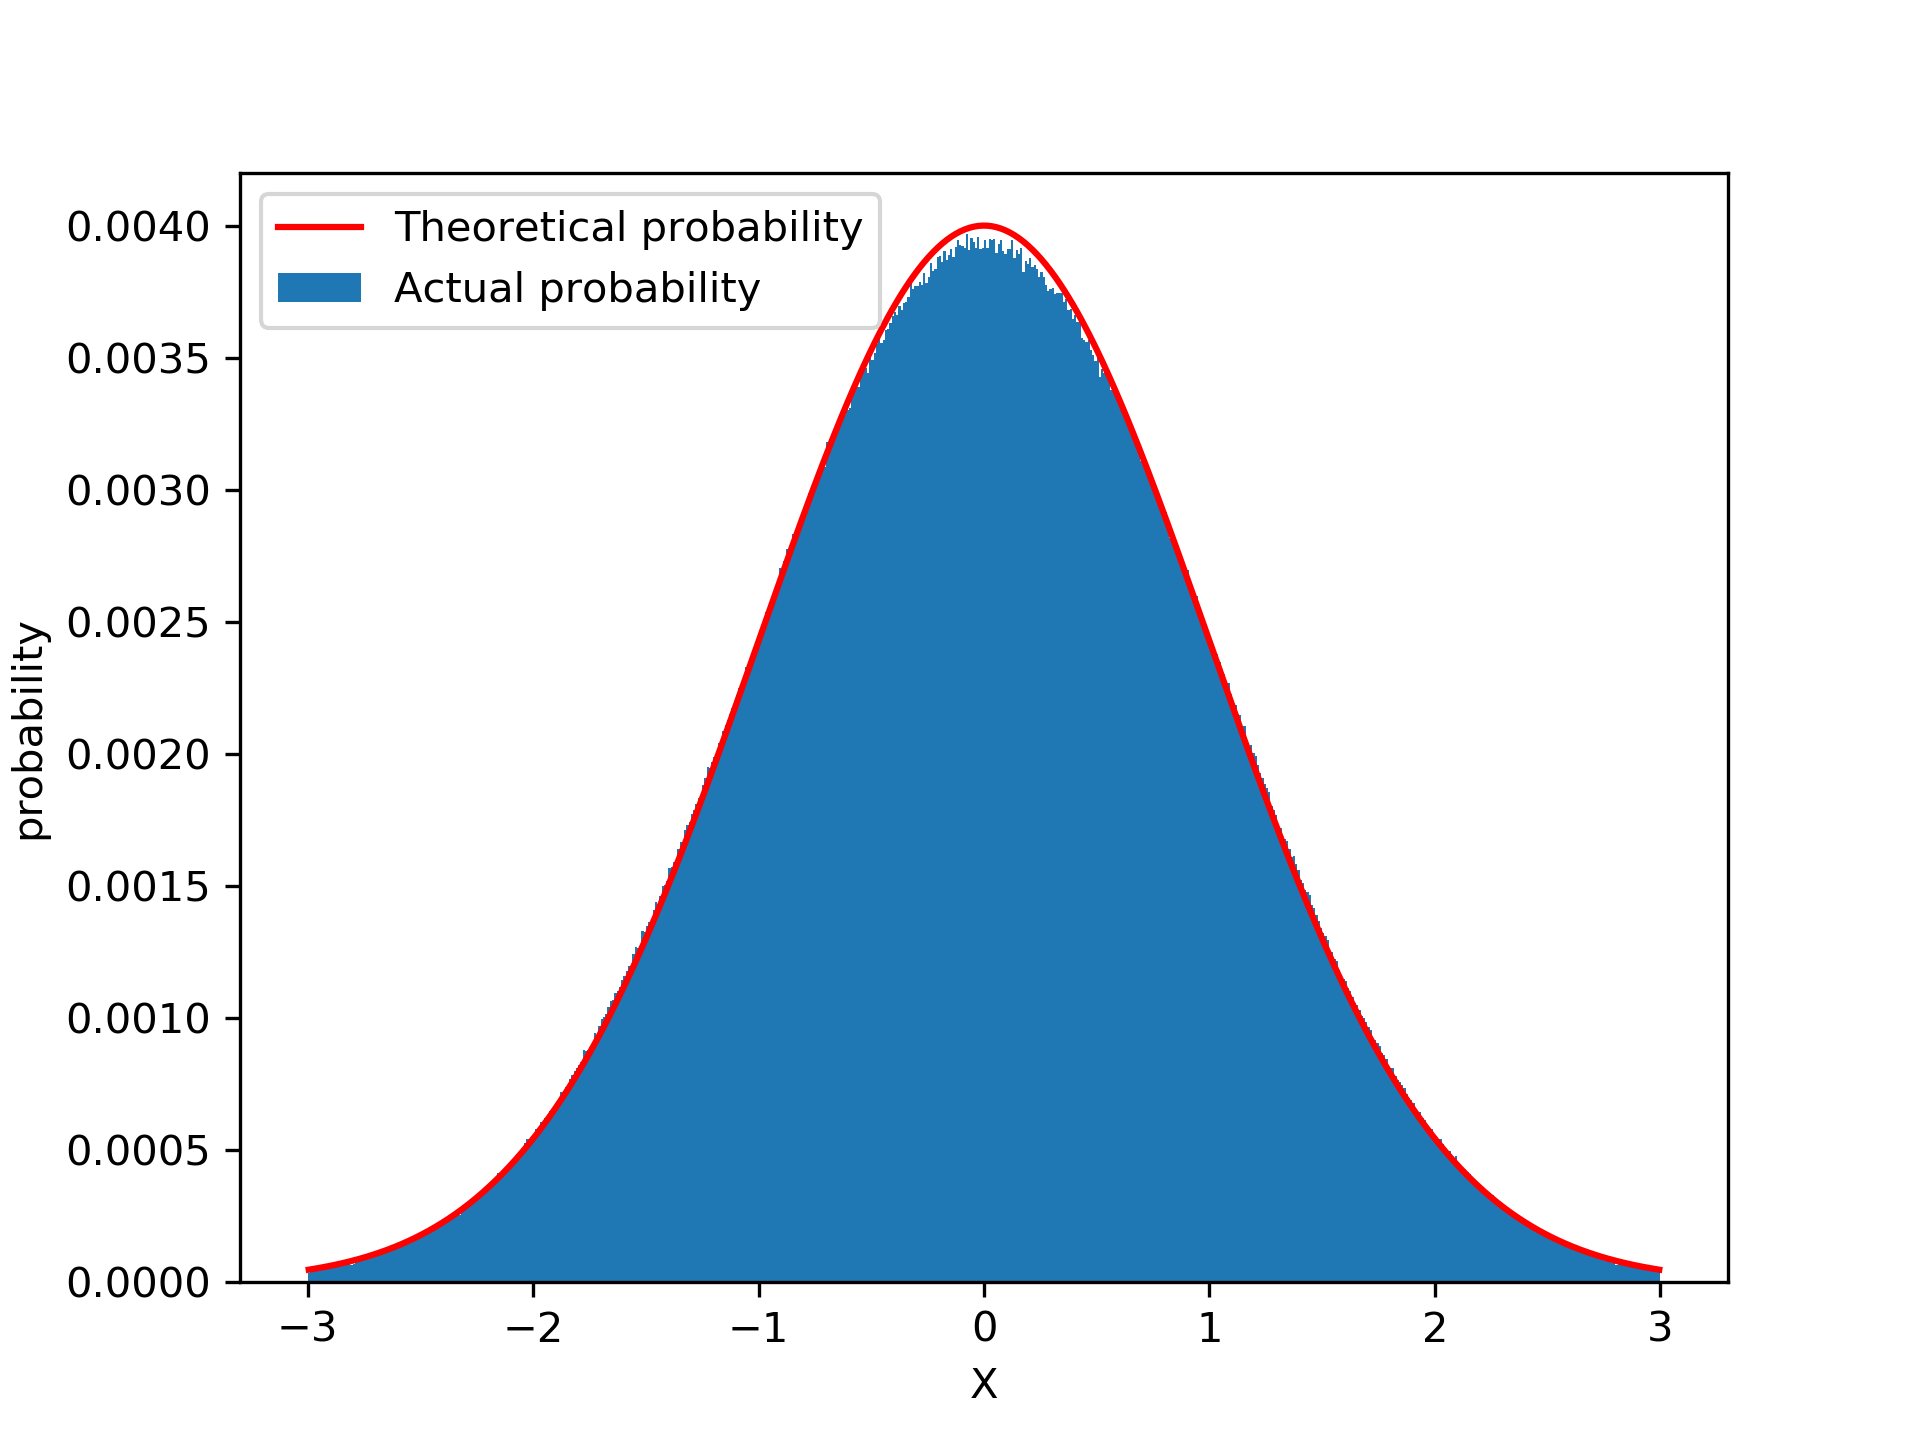
\includegraphics[width=4cm] {1-7-5.png}
}      
\subfigure[每次抽样10个点]{
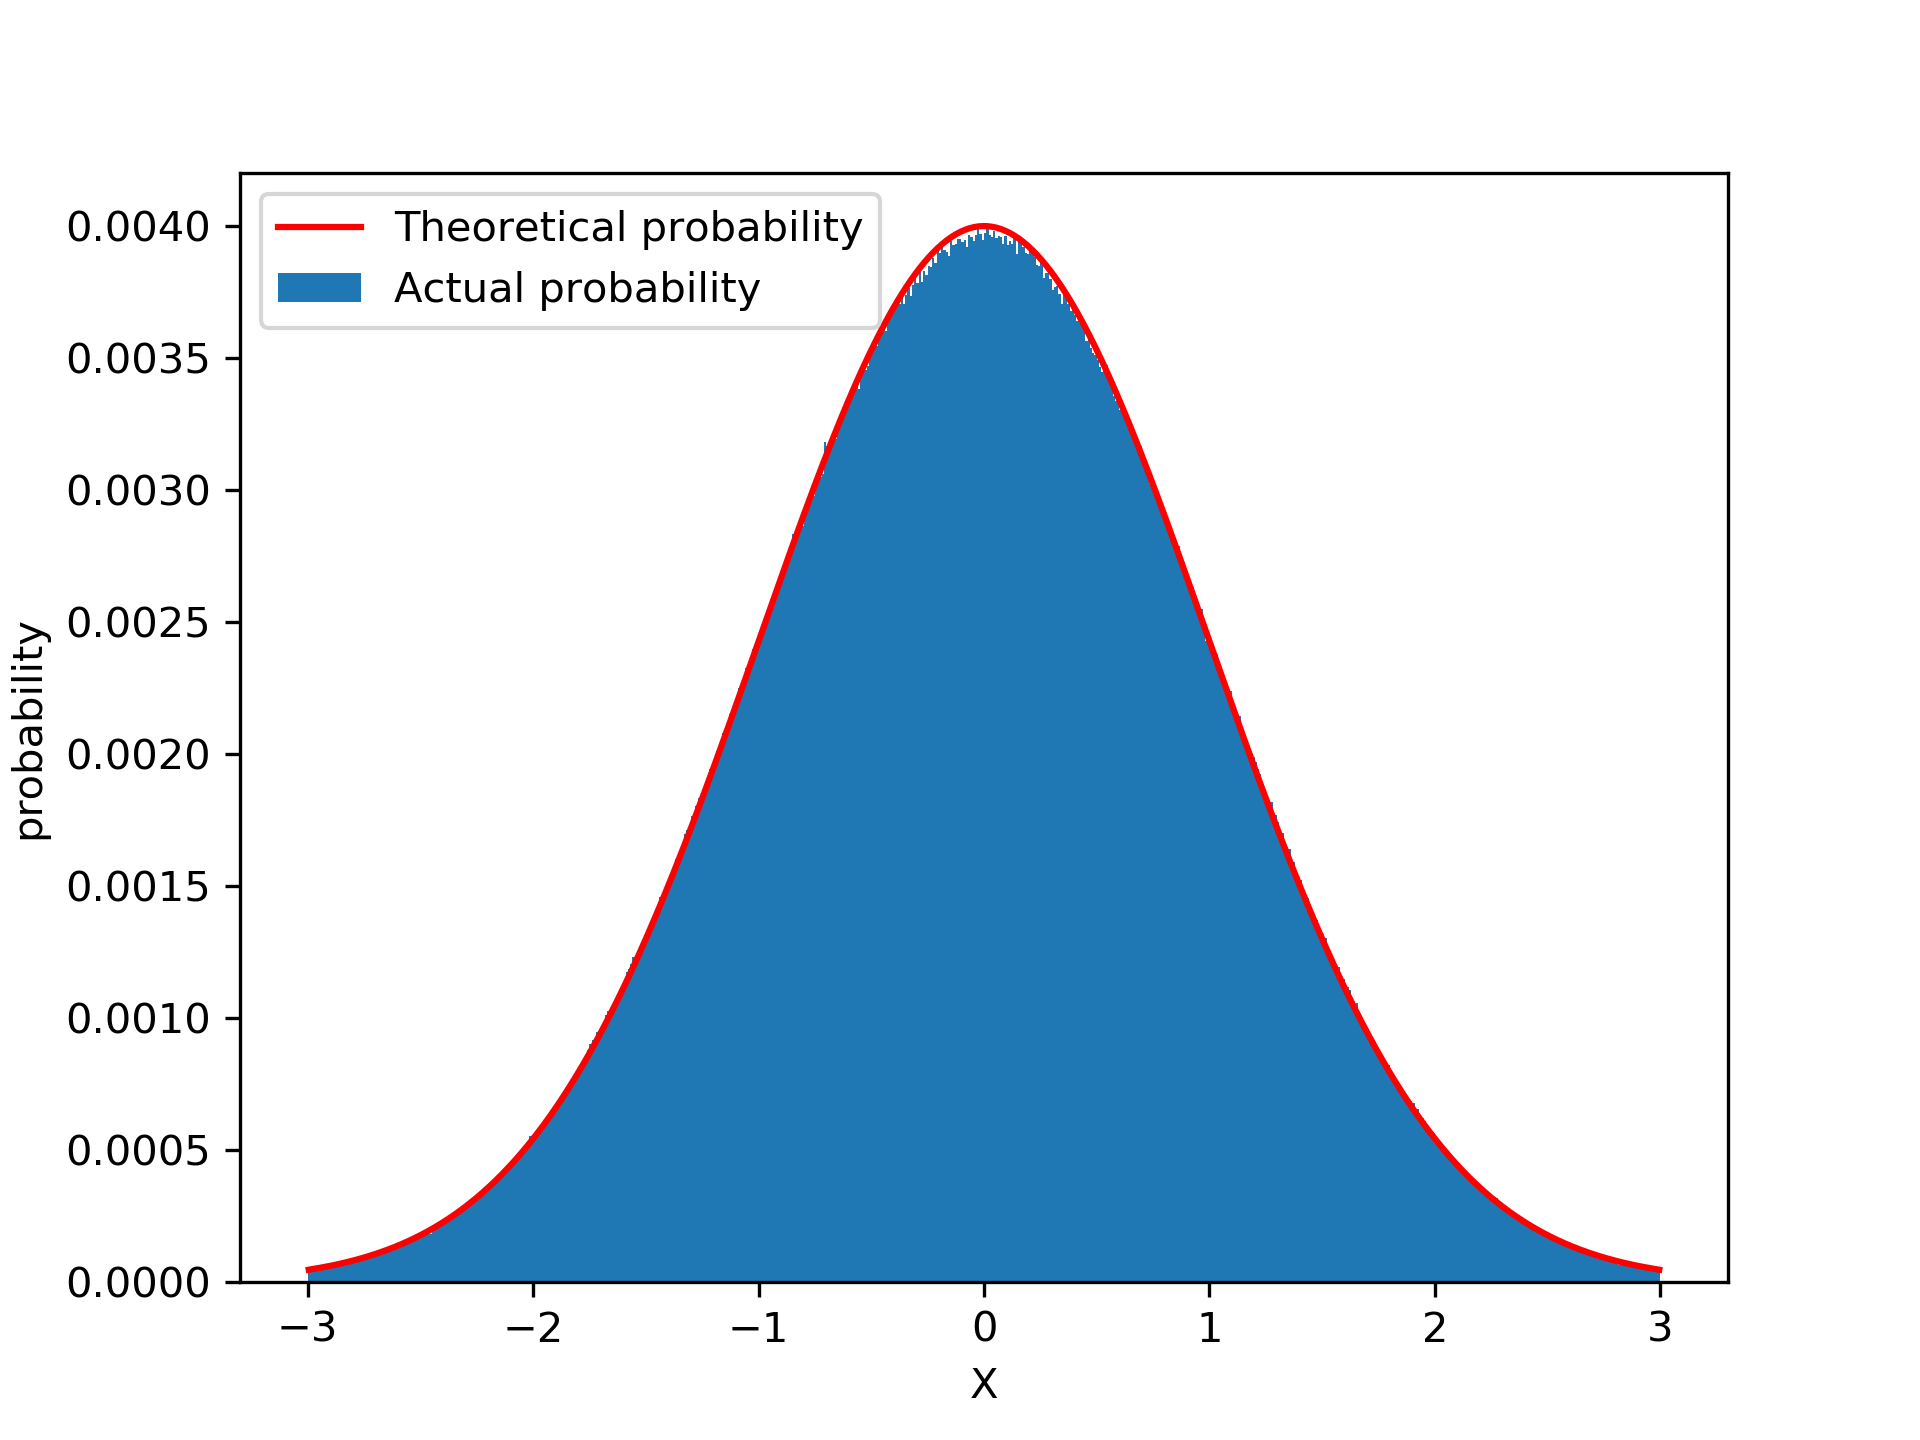
\includegraphics[width=4cm] {1-7-10.png}
}      
\caption{1号分布计算$10^{7}$次后的结果}      
\end{figure}


\begin{figure}[!htbp]   
\centering     
\subfigure[每次抽样2个点]{
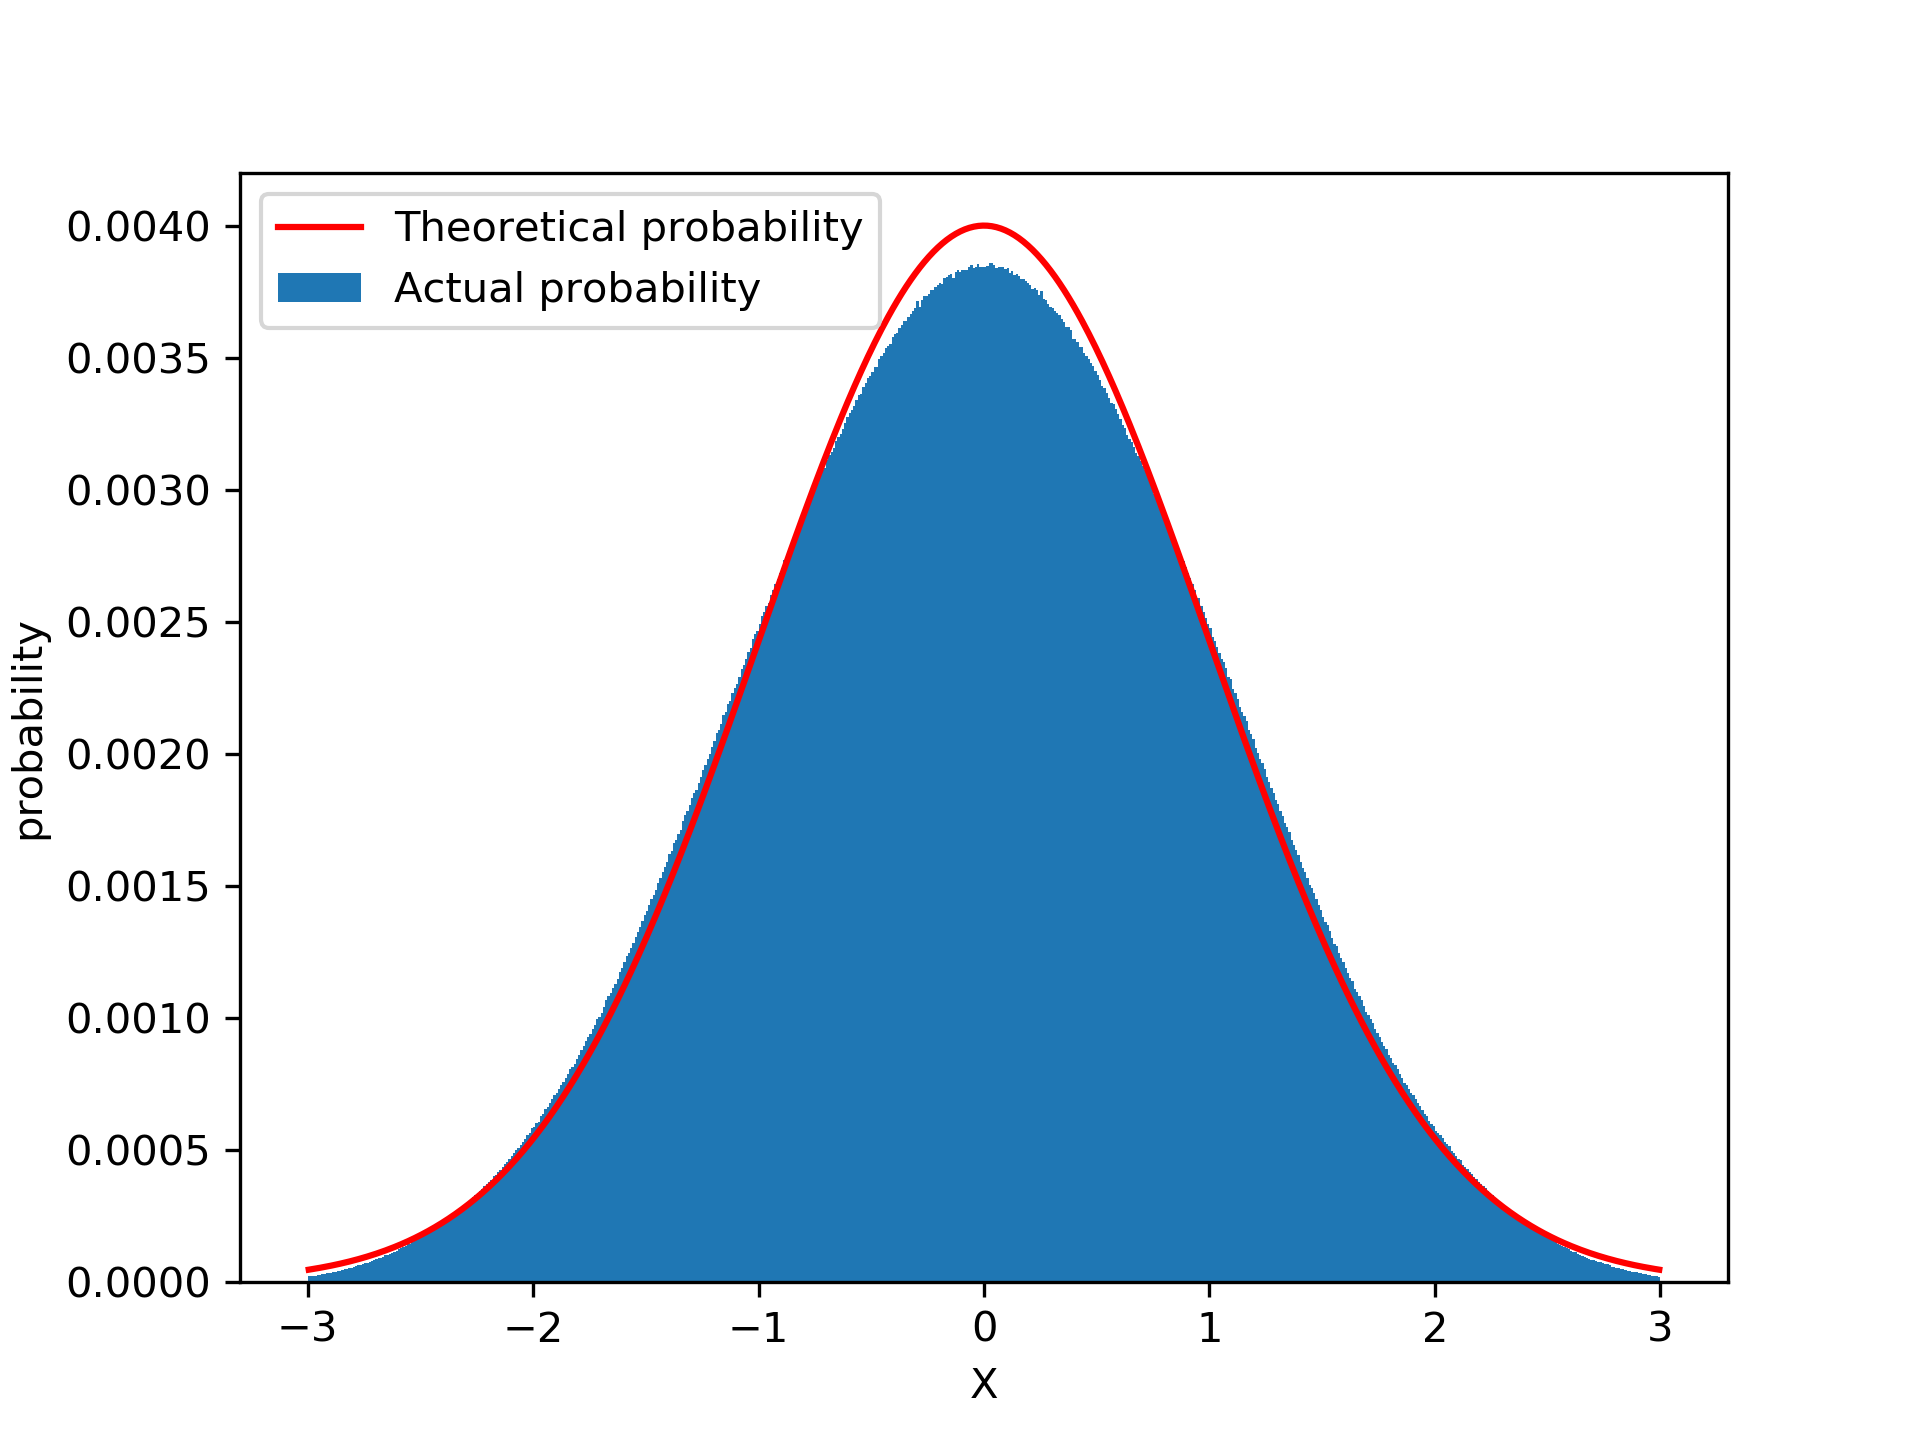
\includegraphics[width=4cm] {1-8-2.png}
}
\subfigure[每次抽样5个点]{
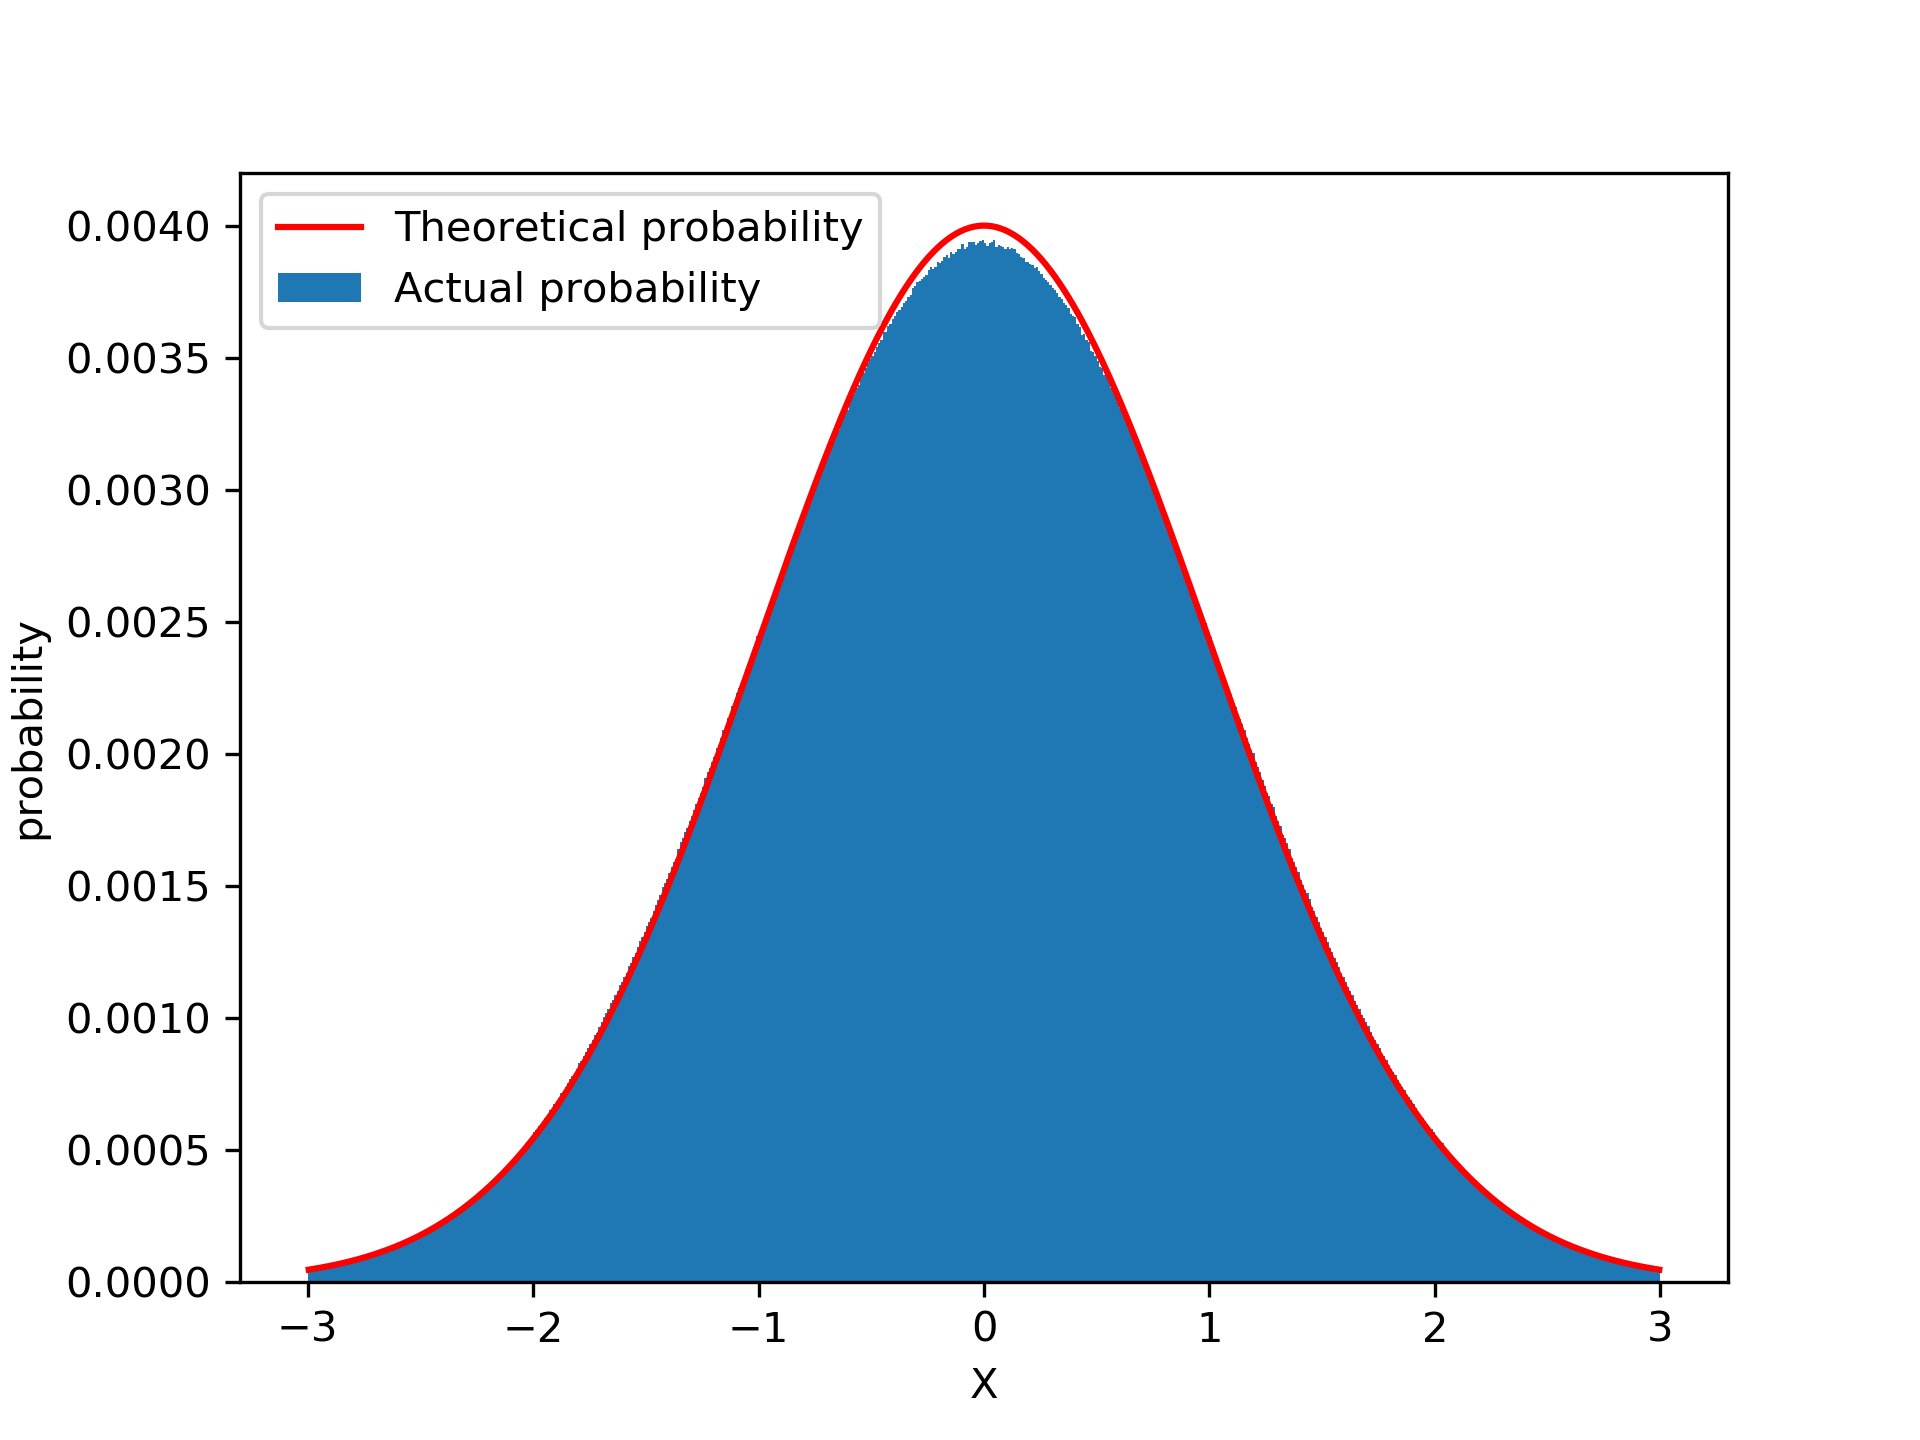
\includegraphics[width=4cm] {1-8-5.png}
}      
\subfigure[每次抽样10个点]{
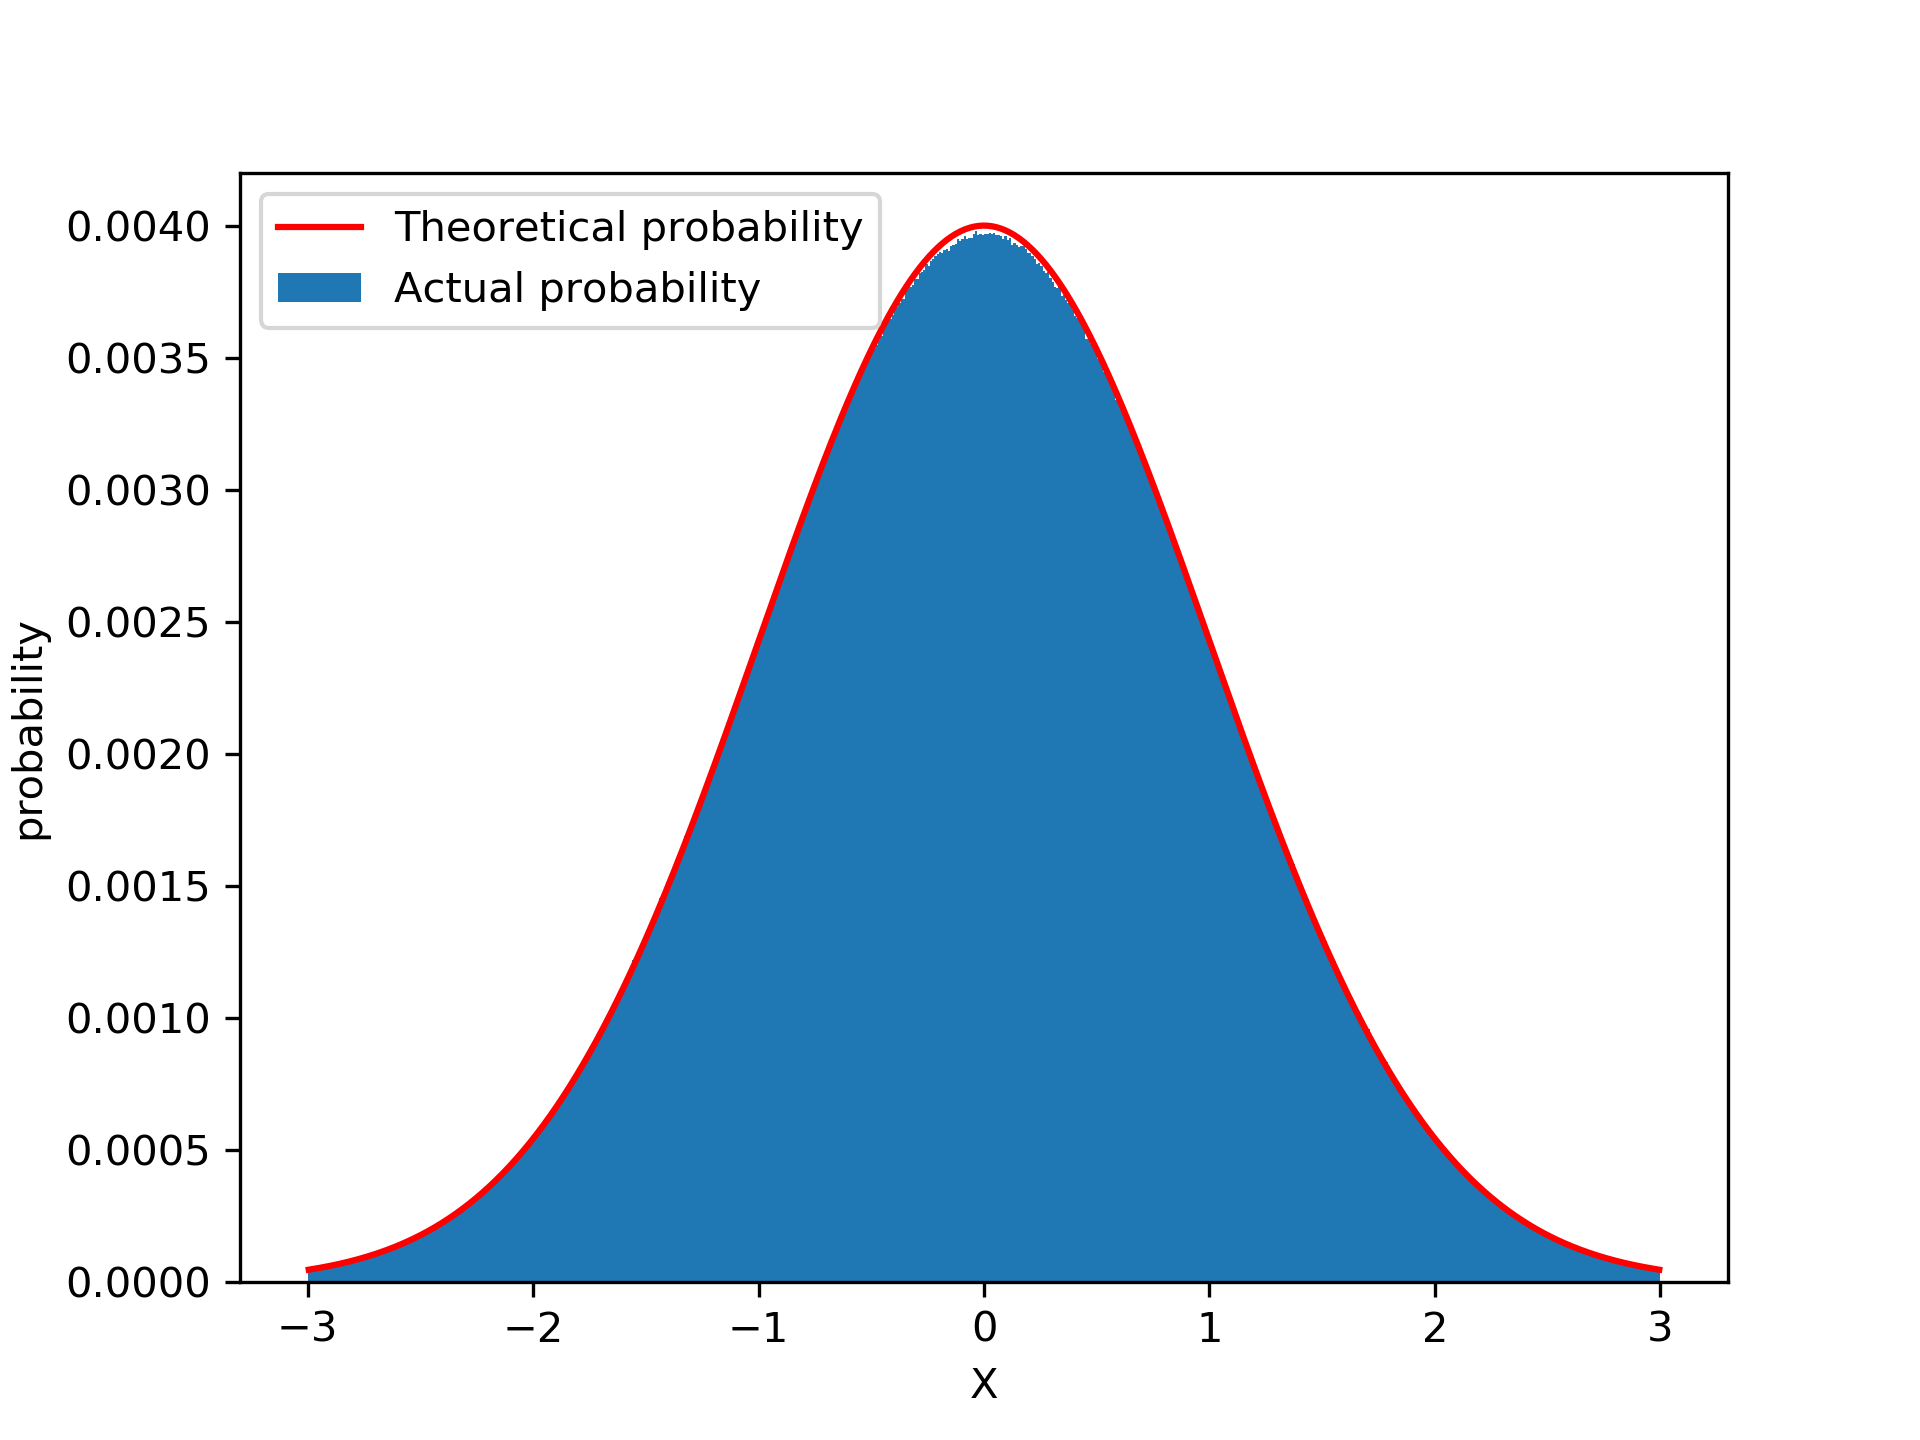
\includegraphics[width=4cm] {1-8-10.png}
}      
\caption{1号分布计算$10^{8}$次后的结果}      
\end{figure}

\newpage 可以看出对于一号分布,随着计算次数和每次抽样个数的增加,其统计量的分布与标准正态分布越来越接近。\footnote{计算次数控制的为对某每次抽样个数确定的统计量的概率分布精确度,次数越多,其与统计量的理论概率分布约接近,下同。}

\begin{figure}[!htbp]   
\centering     
\subfigure[每次抽样2个点]{
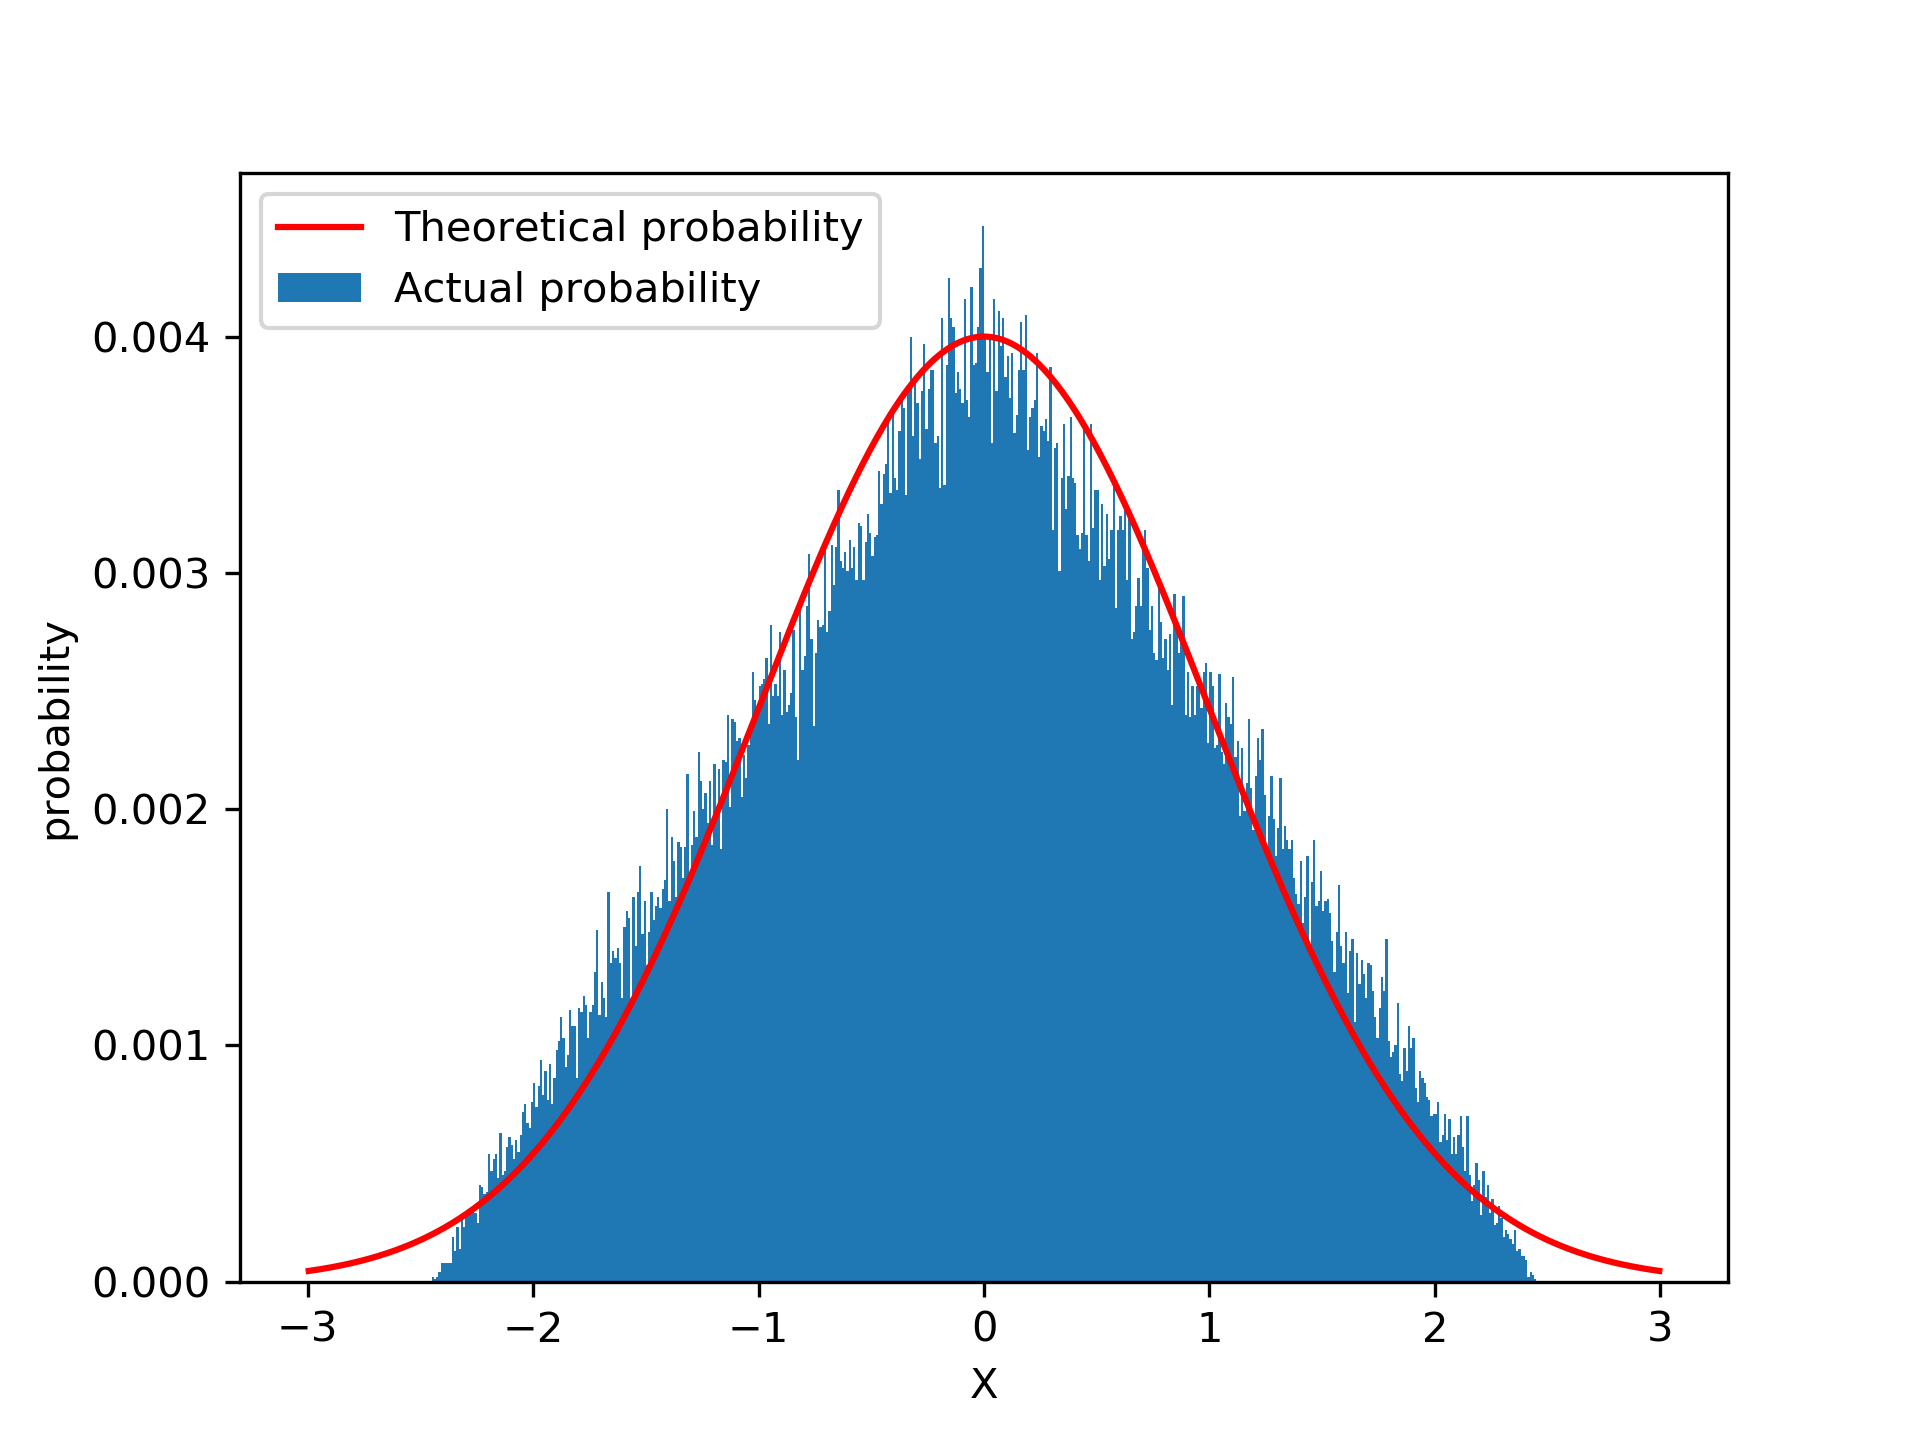
\includegraphics[width=4cm] {2-5-2.png}
}
\subfigure[每次抽样5个点]{
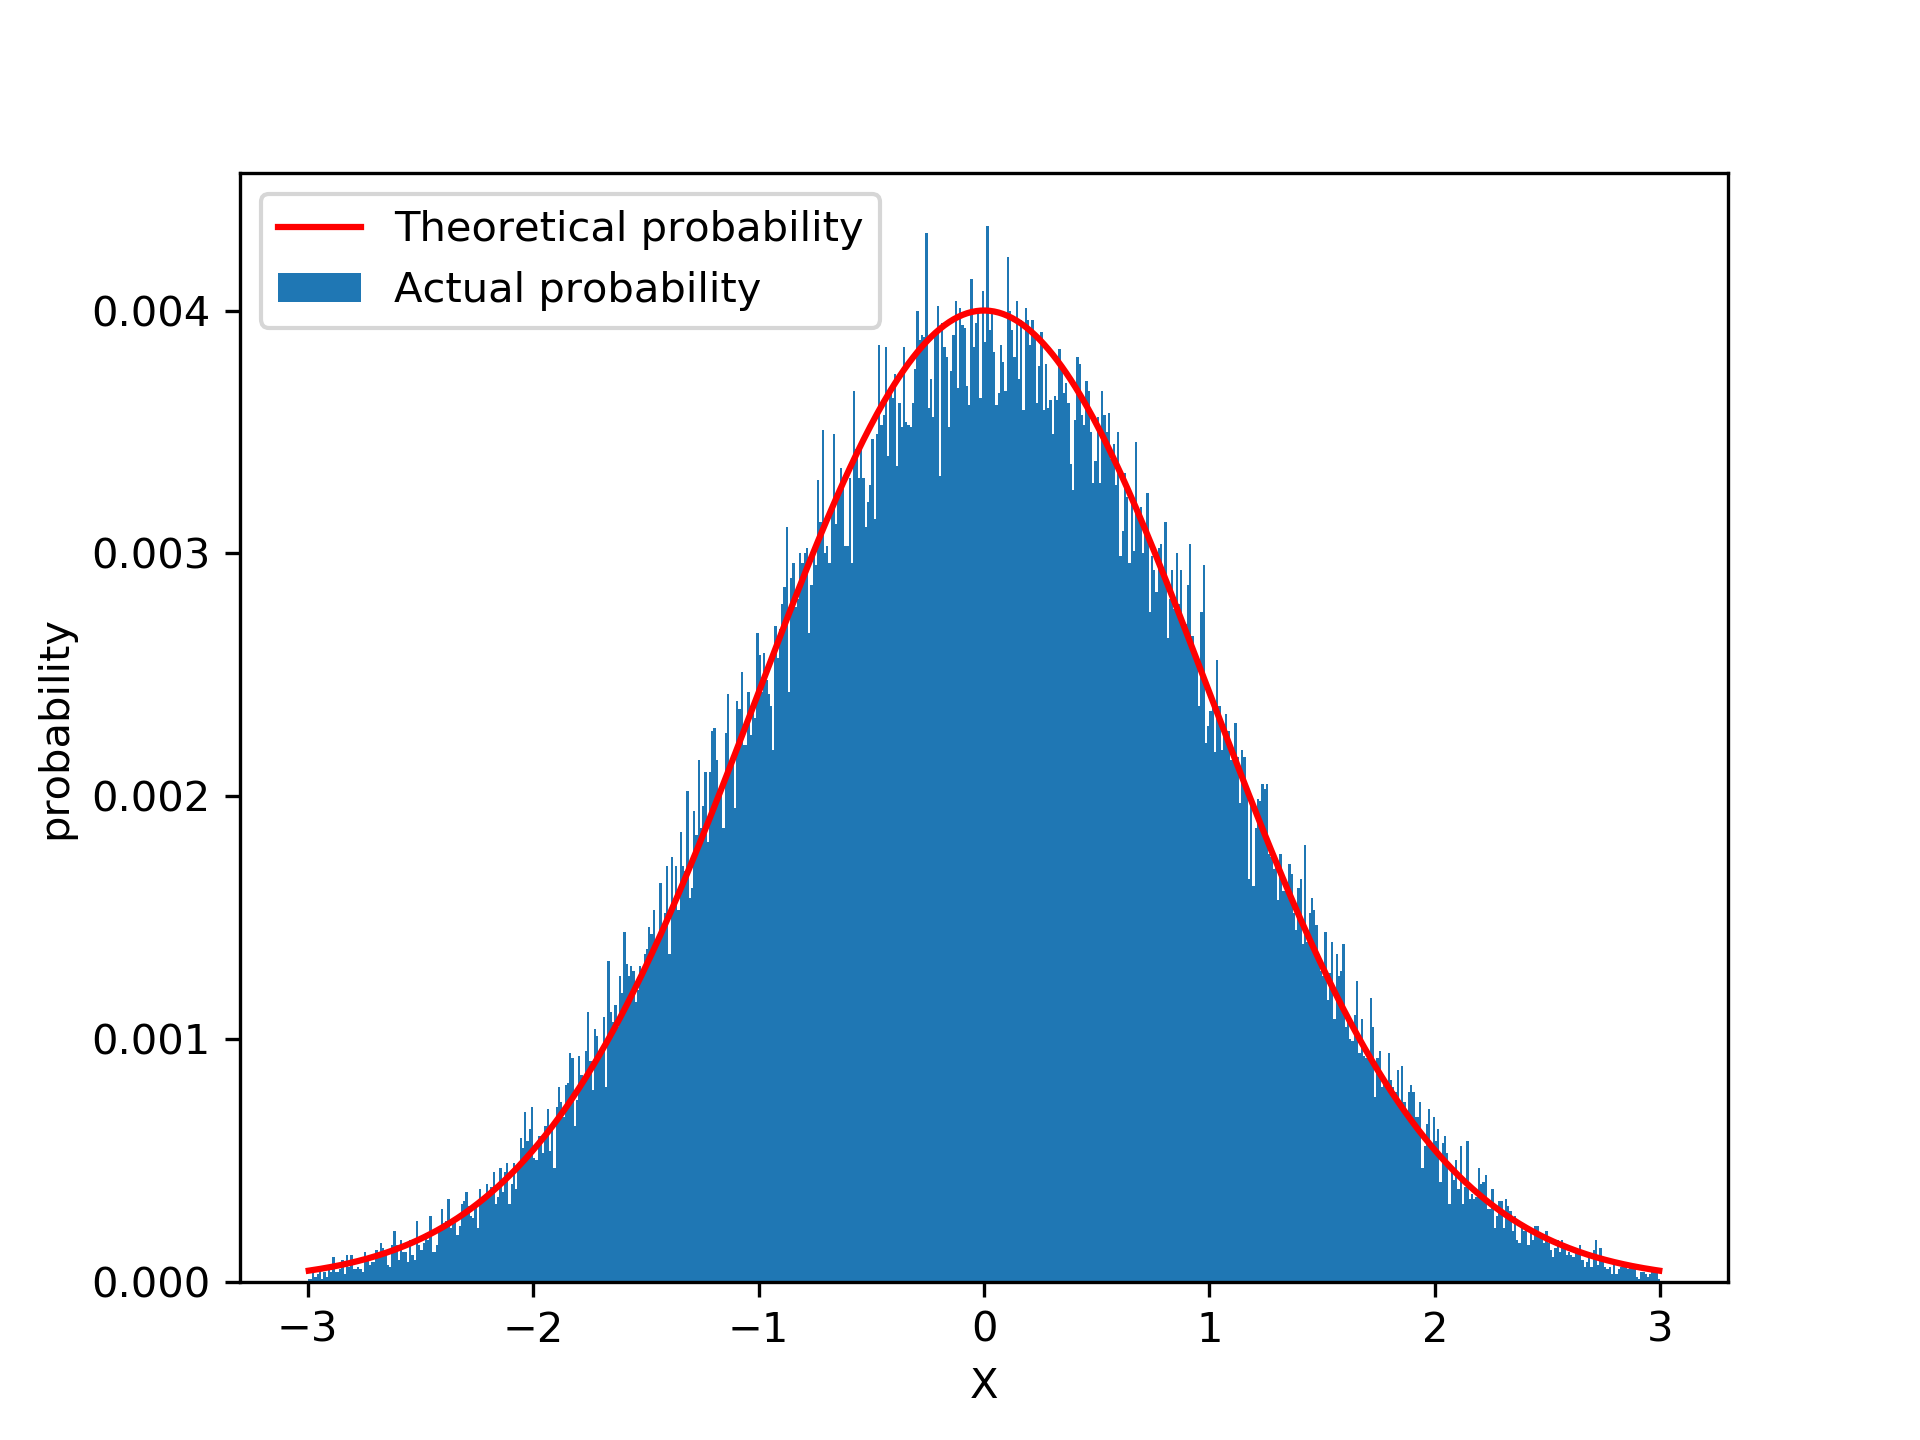
\includegraphics[width=4cm] {2-5-5.png}
}      
\subfigure[每次抽样10个点]{
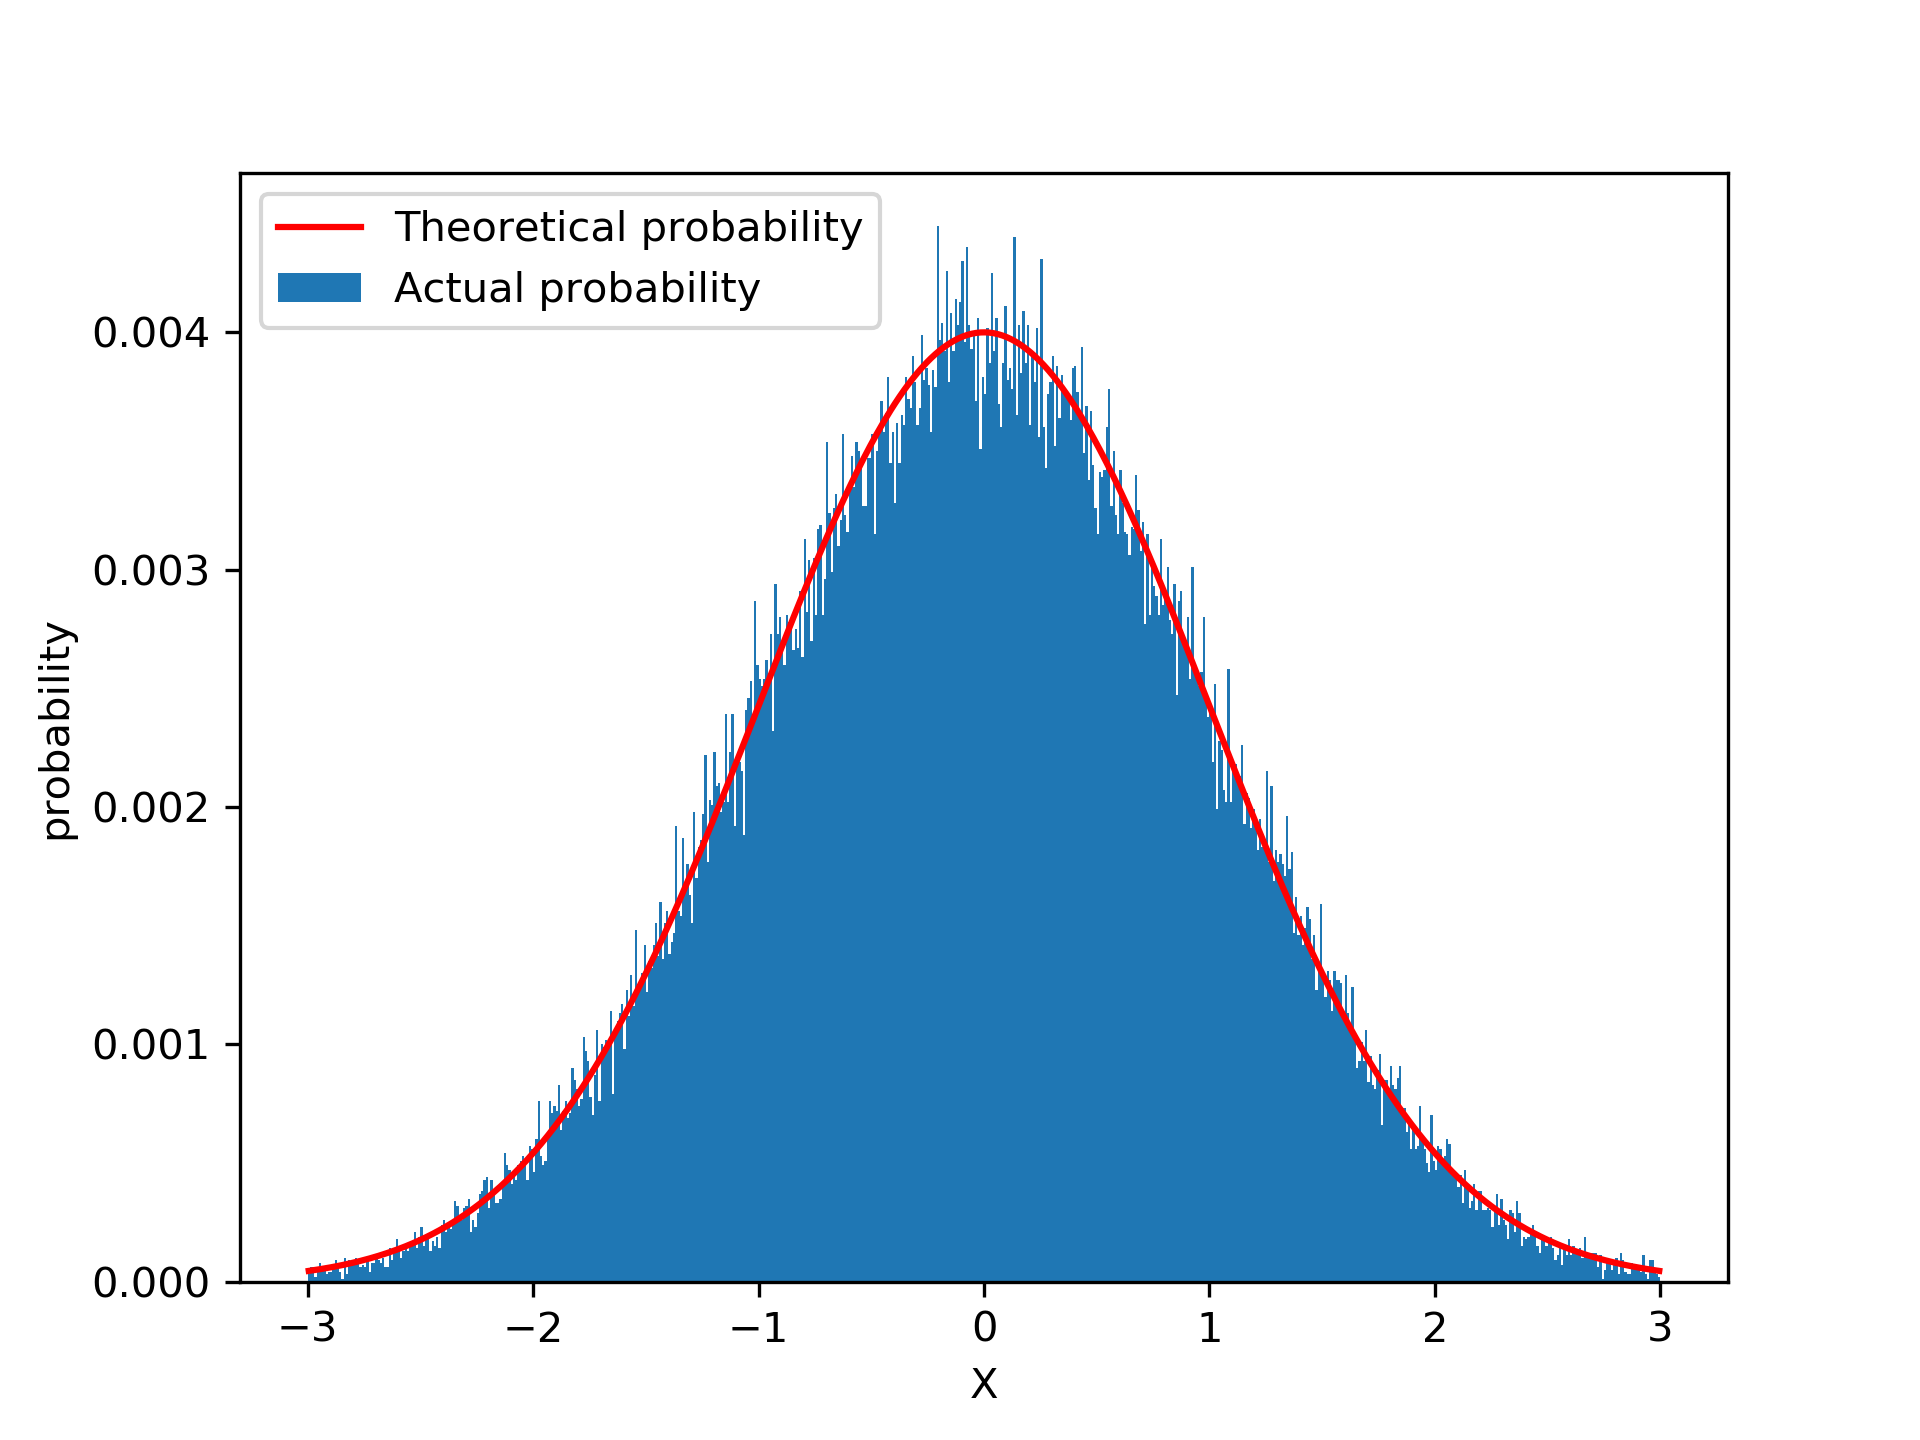
\includegraphics[width=4cm] {2-5-10.png}
}      
\caption{2号分布计算$10^{5}$次后的结果}      
\end{figure}


\begin{figure}[!htbp]   
\centering     
\subfigure[每次抽样2个点]{
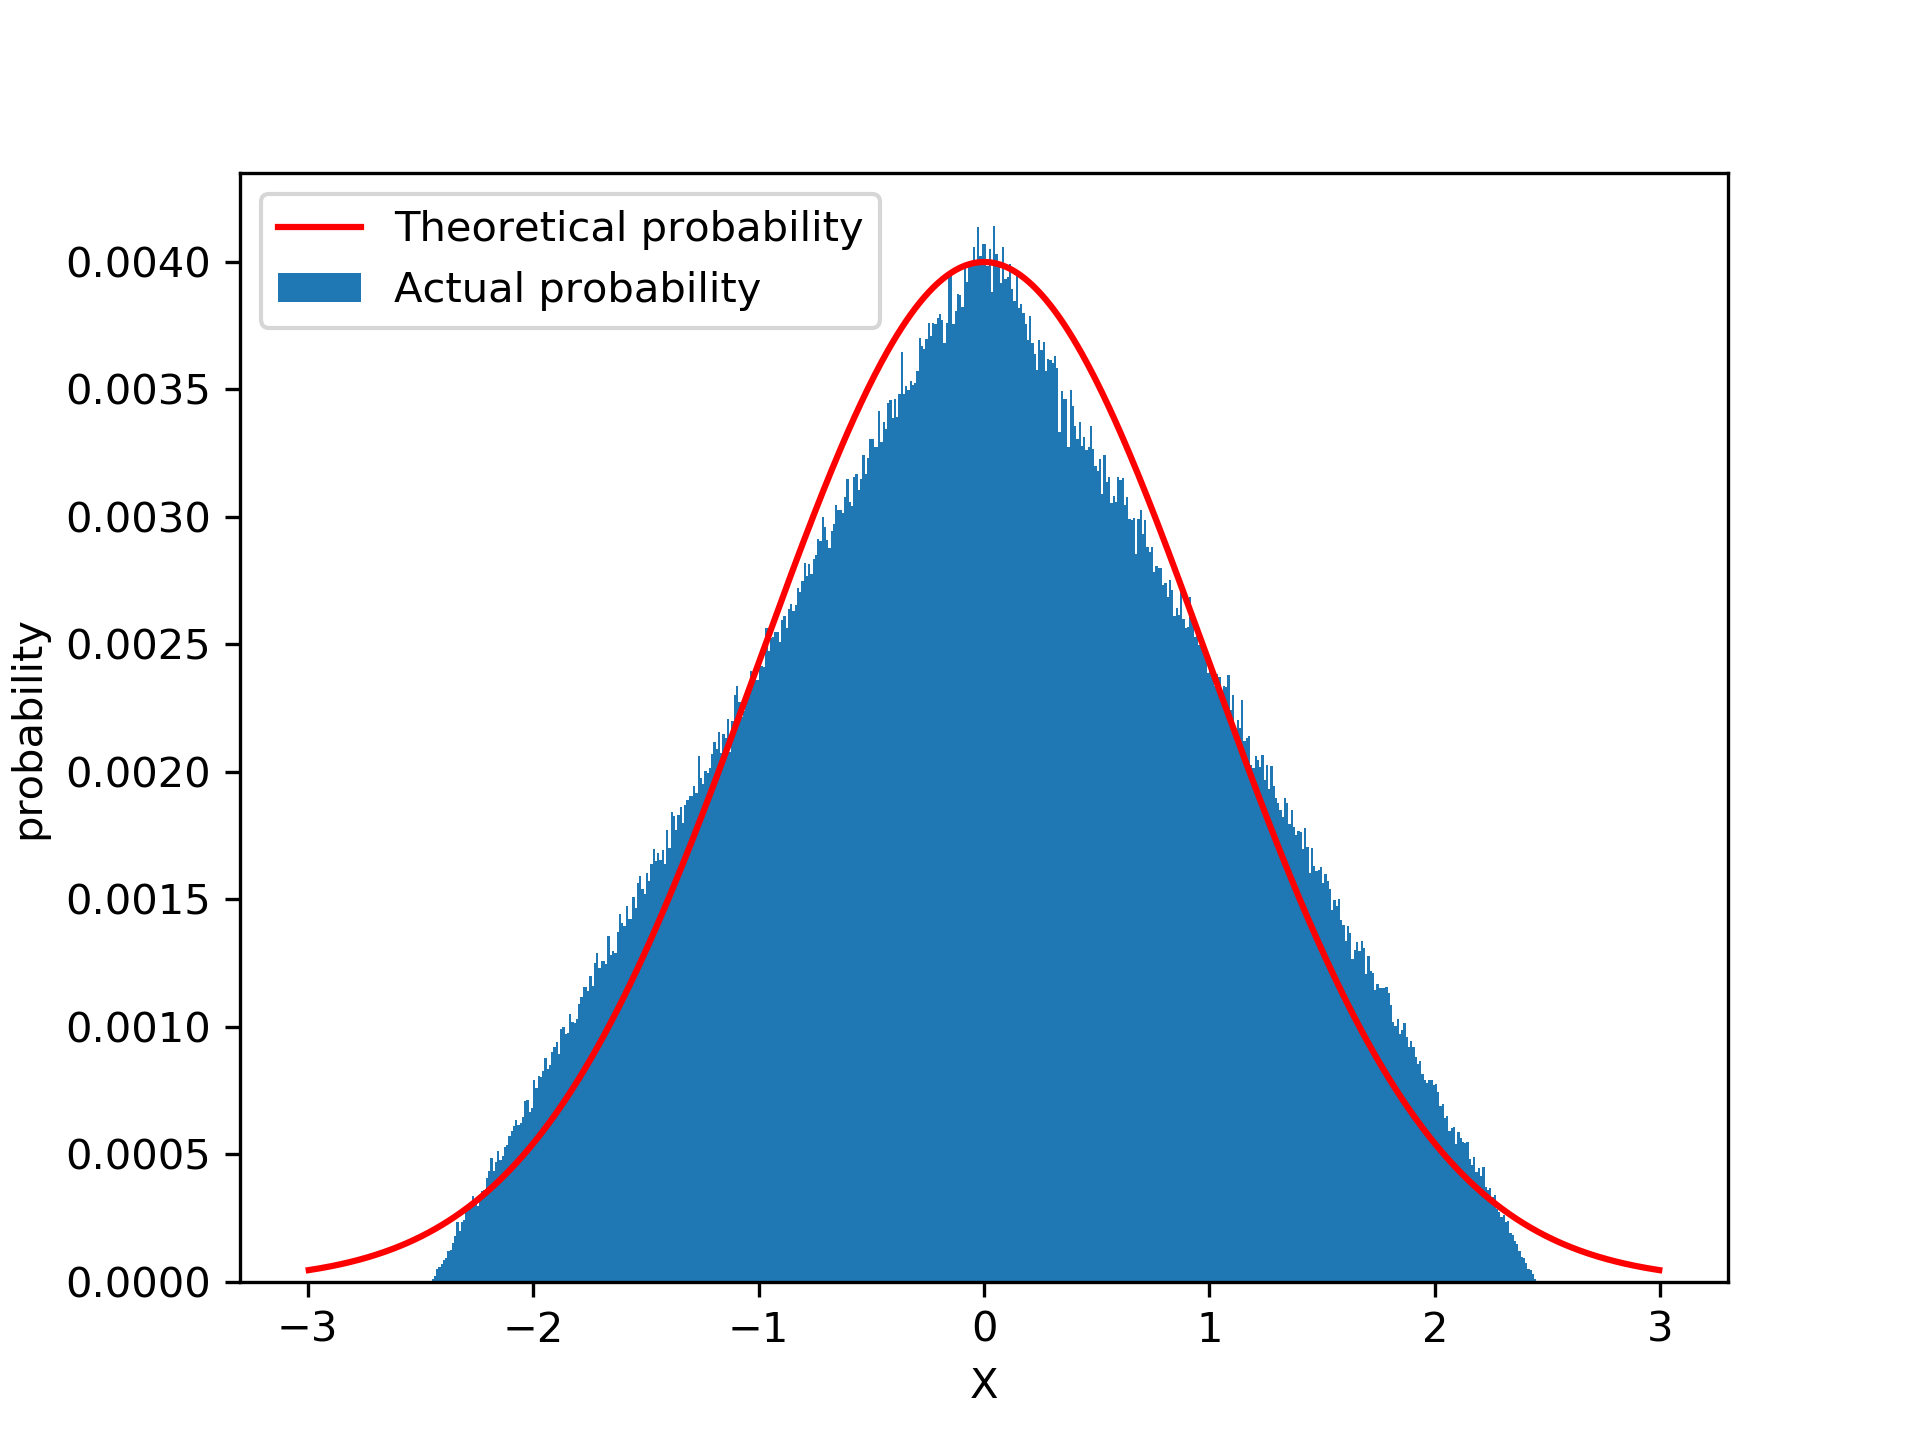
\includegraphics[width=4cm] {2-6-2.png}
}
\subfigure[每次抽样5个点]{
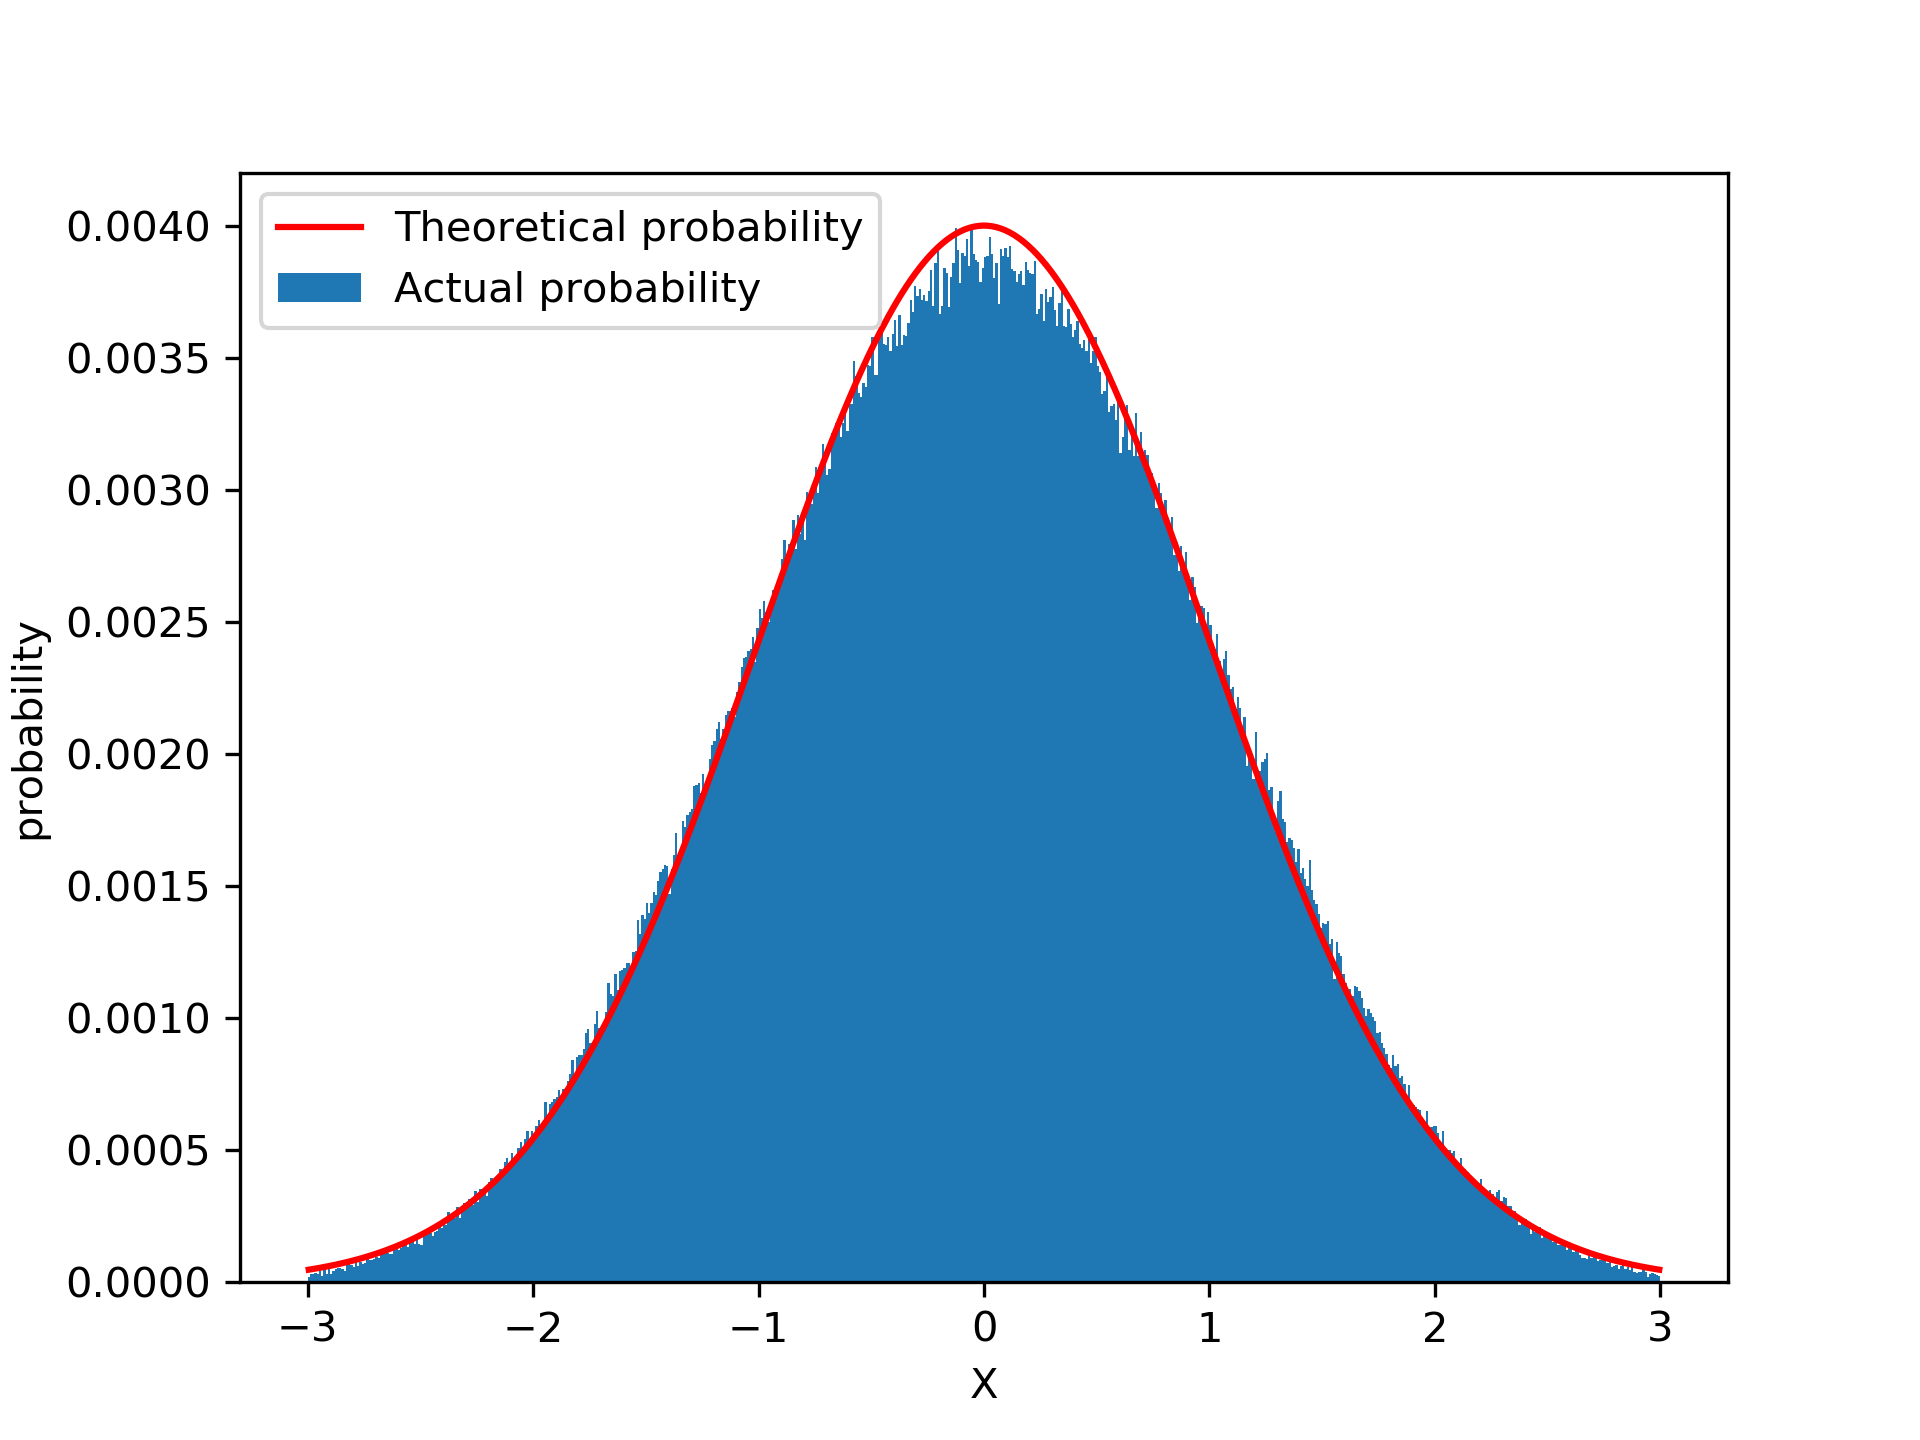
\includegraphics[width=4cm] {2-6-5.png}
}      
\subfigure[每次抽样10个点]{
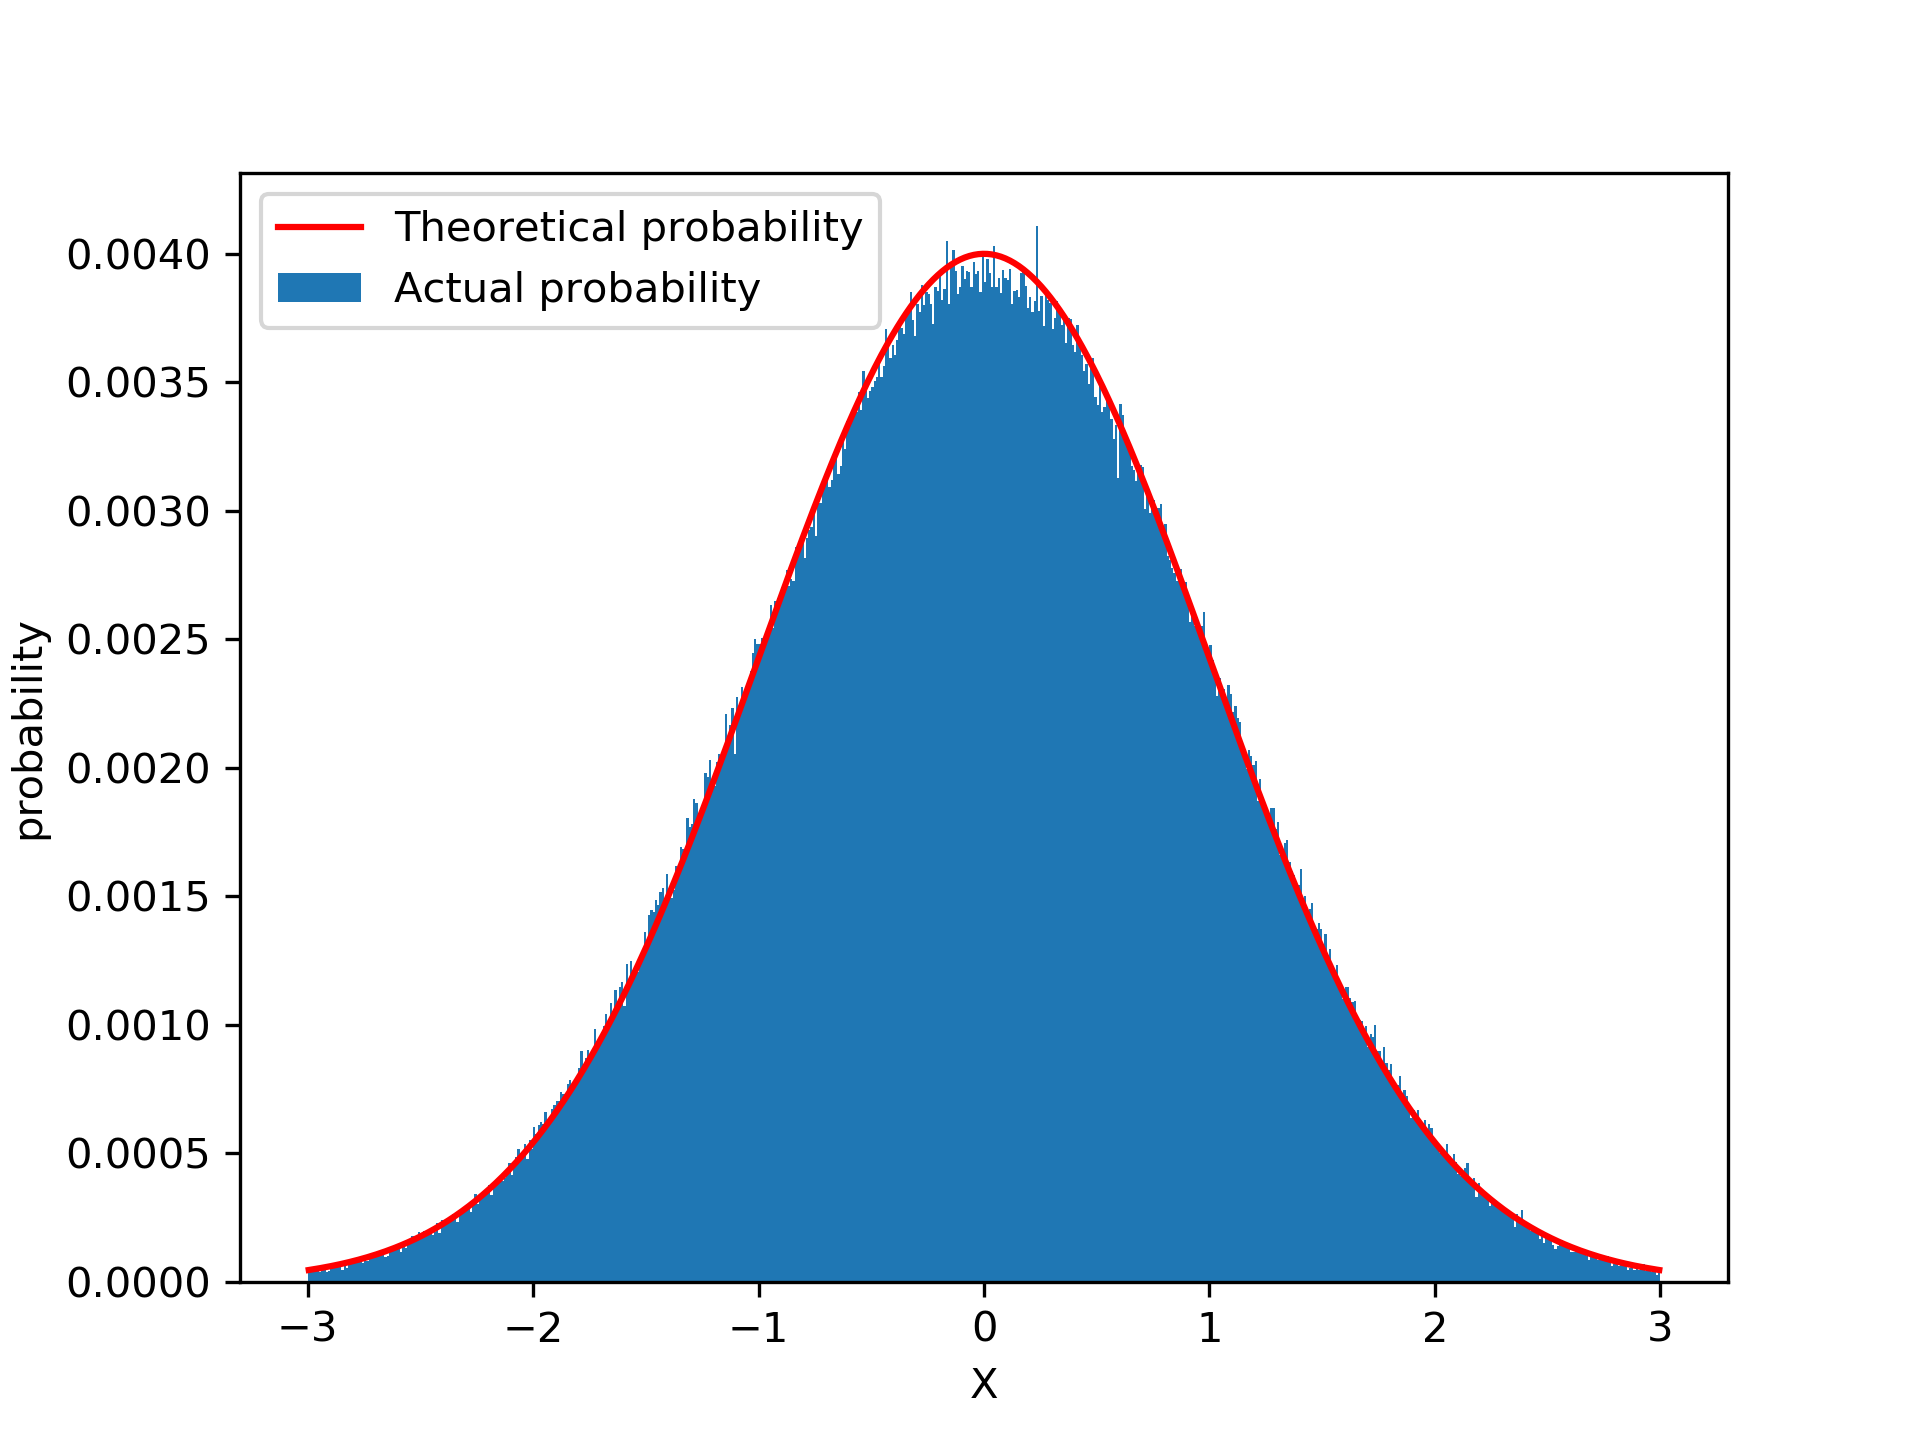
\includegraphics[width=4cm] {2-6-10.png}
}      
\caption{2号分布计算$10^{6}$次后的结果}      
\end{figure}


\begin{figure}[!htbp]   
\centering     
\subfigure[每次抽样2个点]{
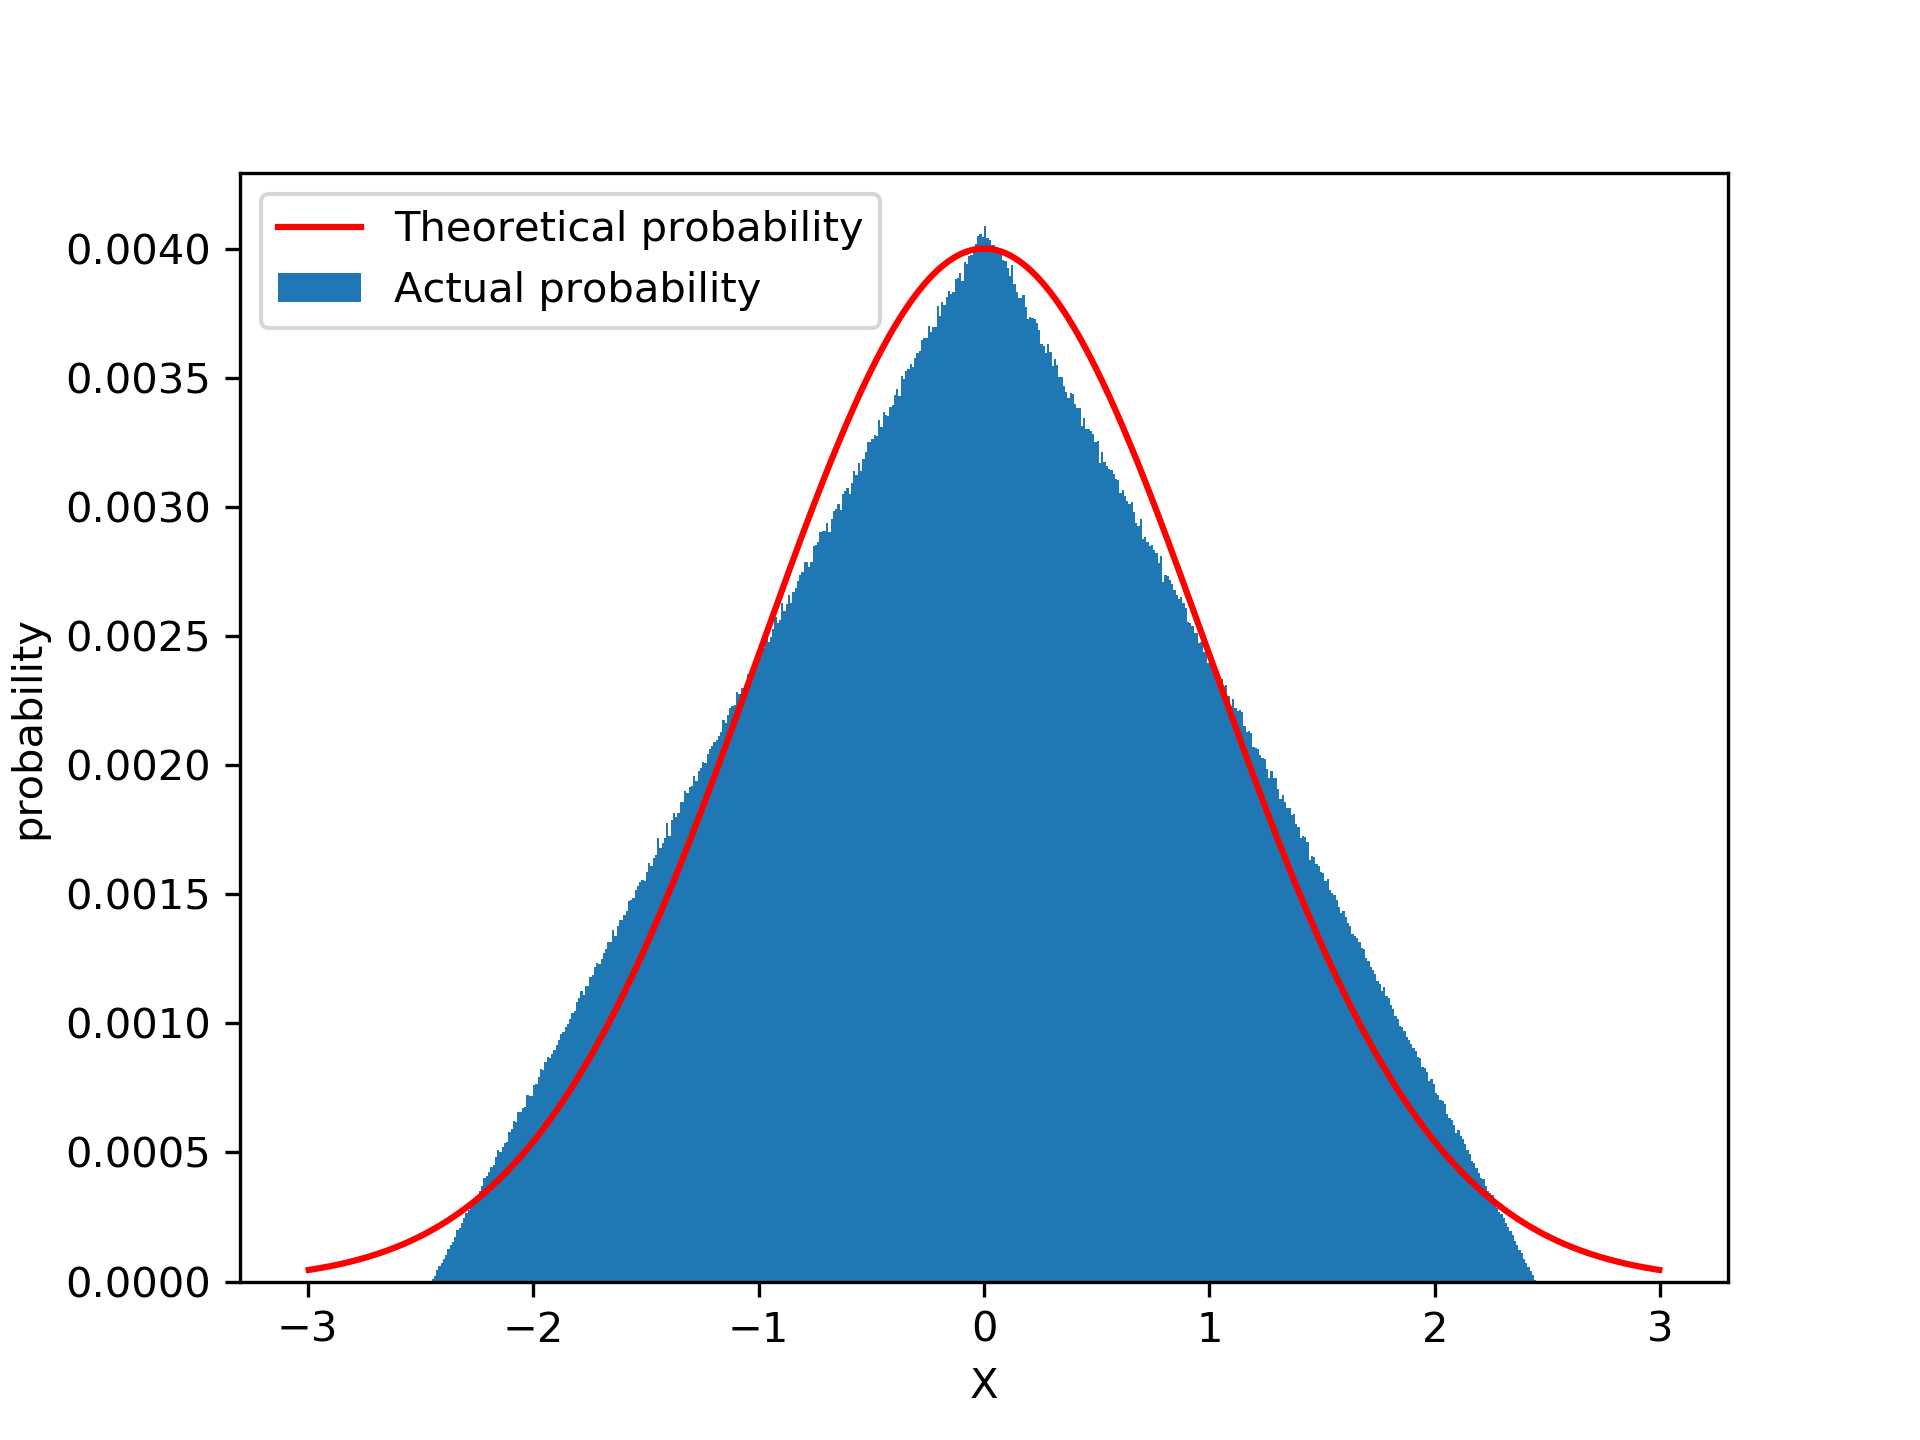
\includegraphics[width=4cm] {2-7-2.png}
}
\subfigure[每次抽样5个点]{
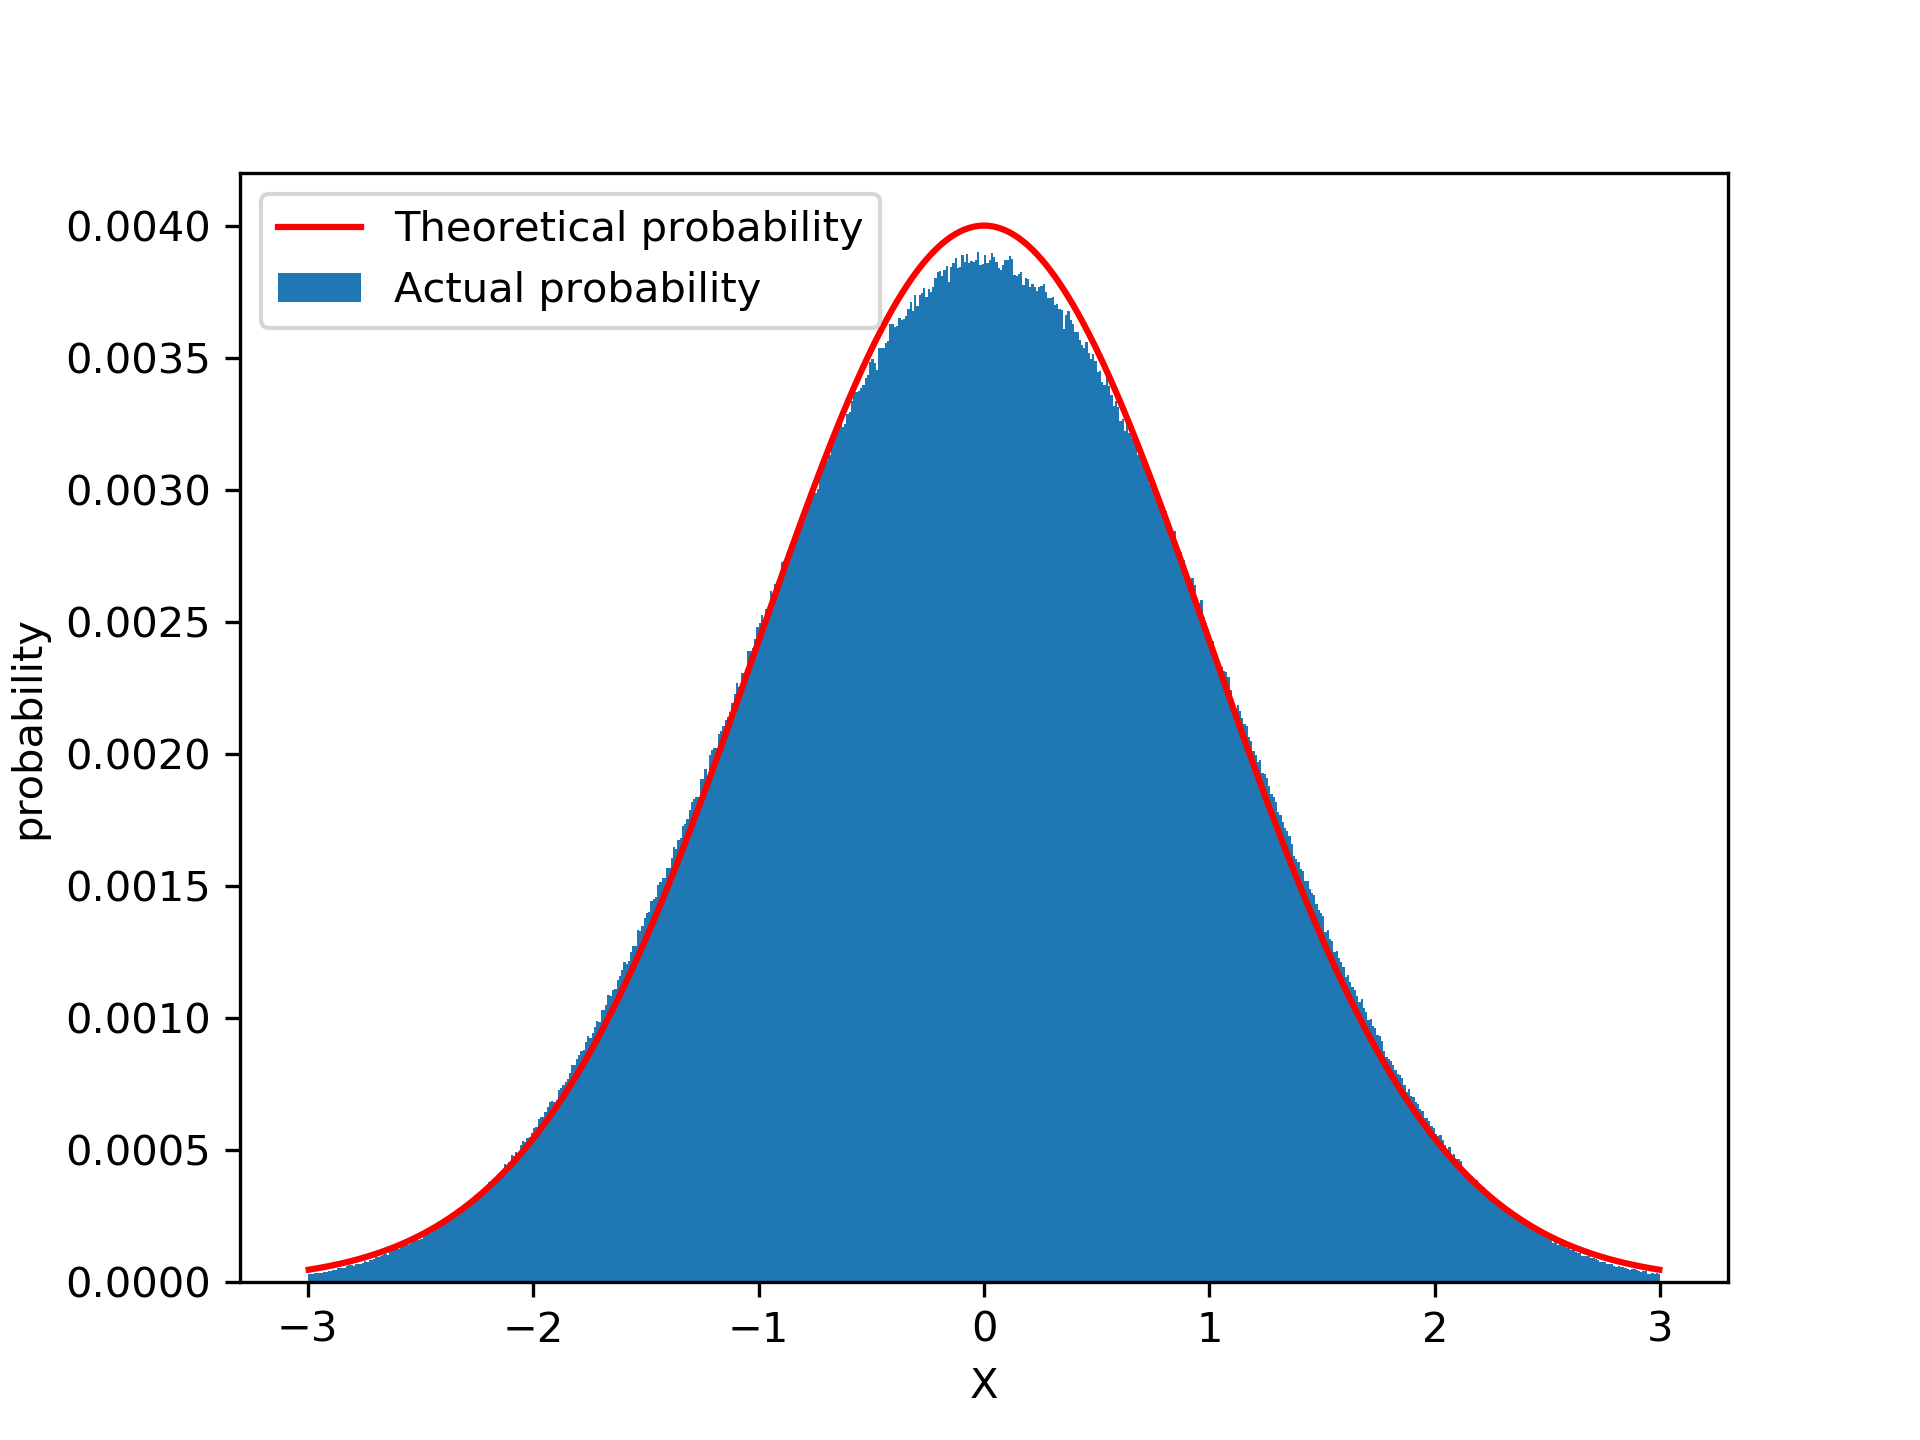
\includegraphics[width=4cm] {2-7-5.png}
}      
\subfigure[每次抽样10个点]{
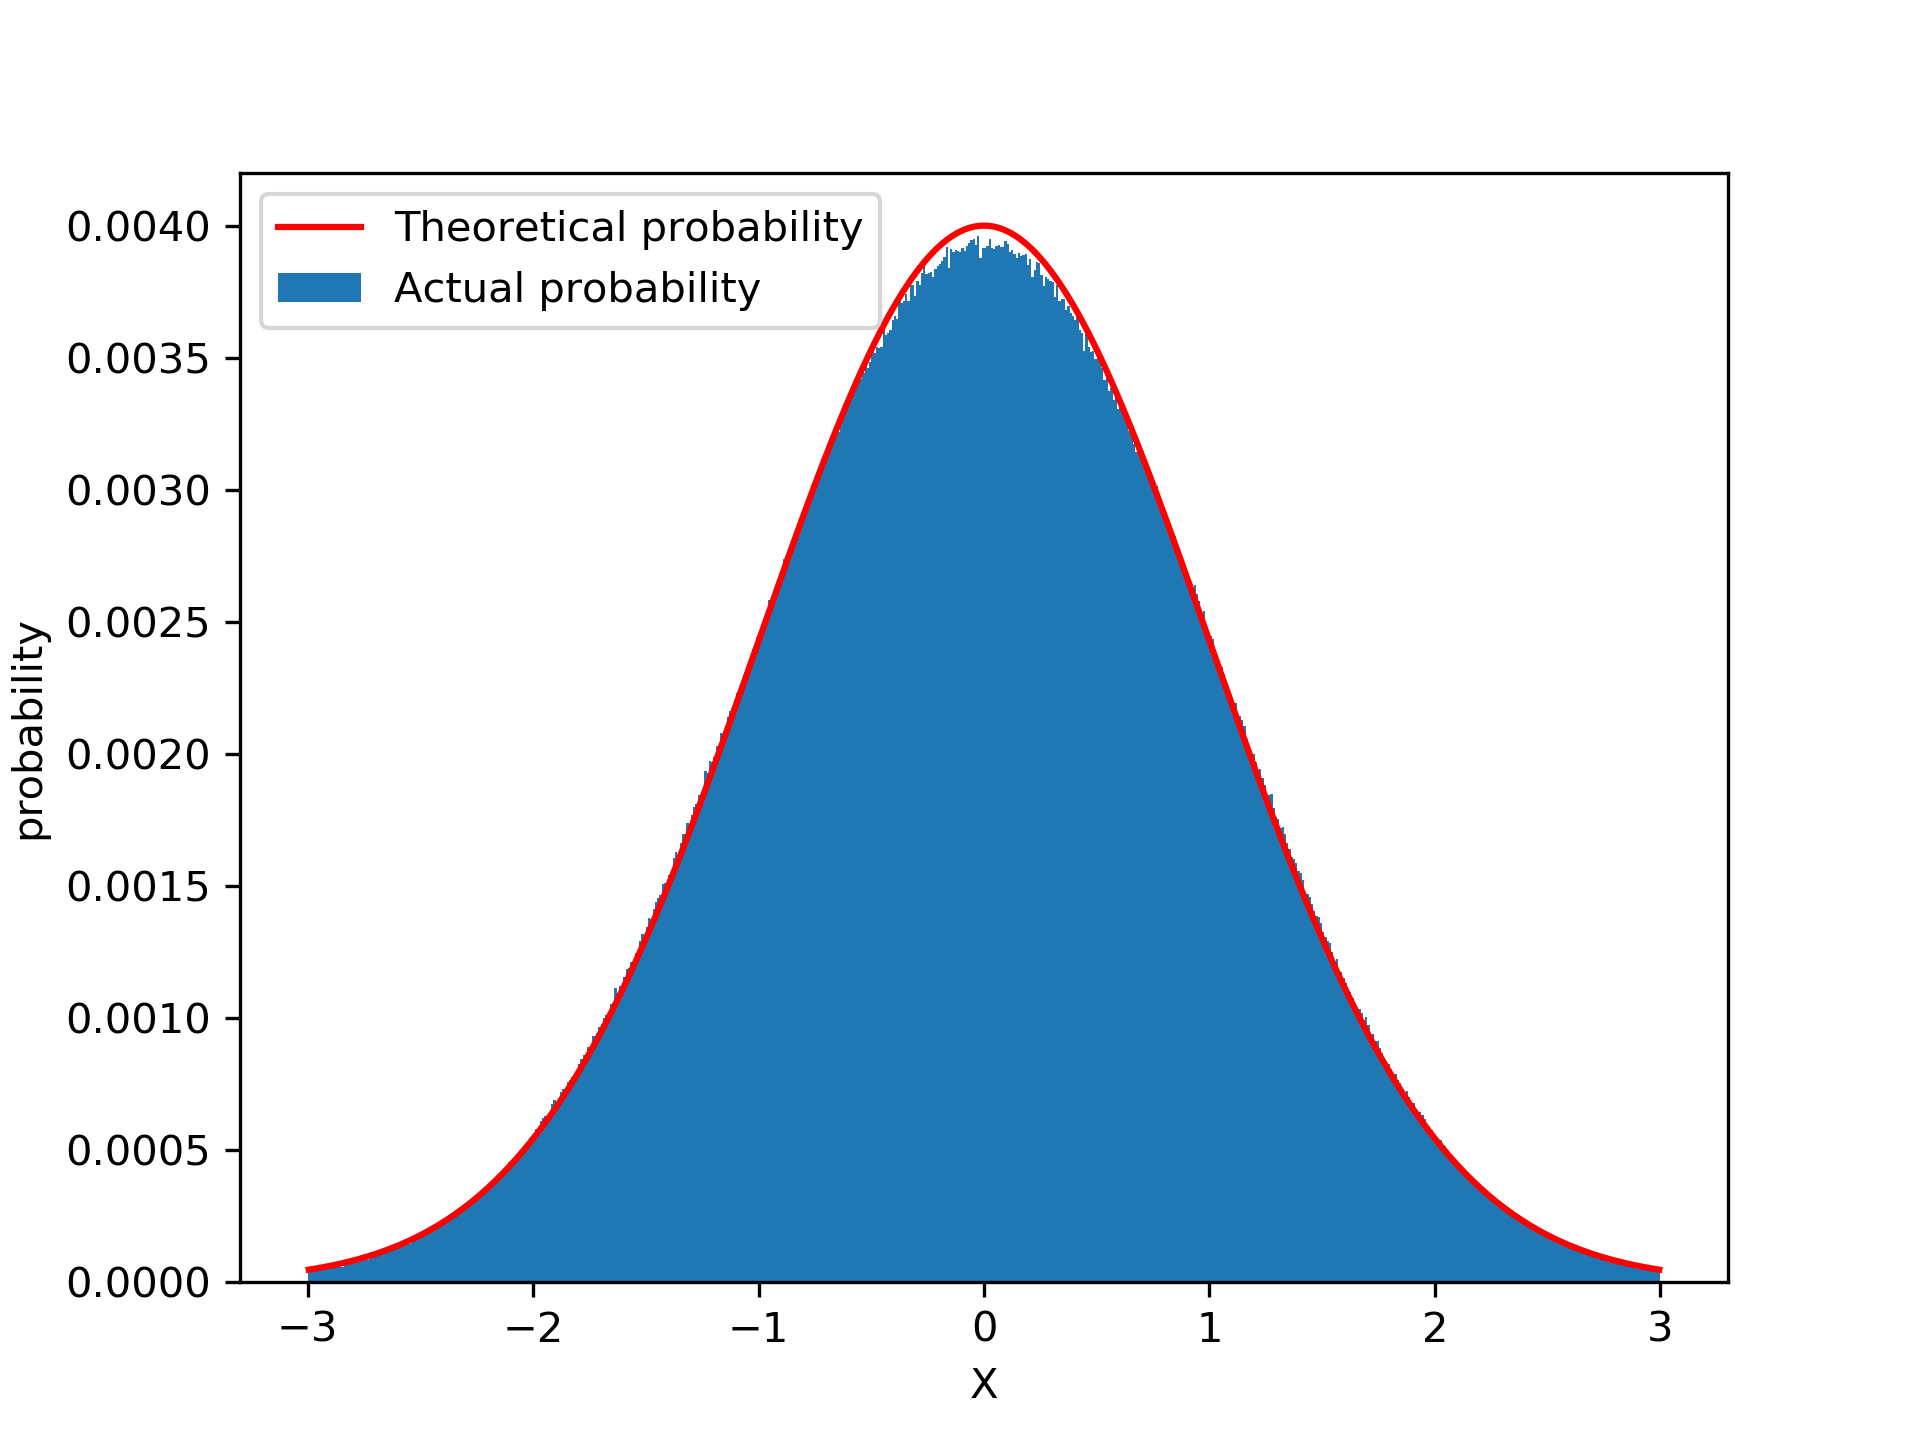
\includegraphics[width=4cm] {2-7-10.png}
}      
\caption{2号分布计算$10^{7}$次后的结果}     
\end{figure}


\begin{figure}[!htbp]   
\centering     
\subfigure[每次抽样2个点]{
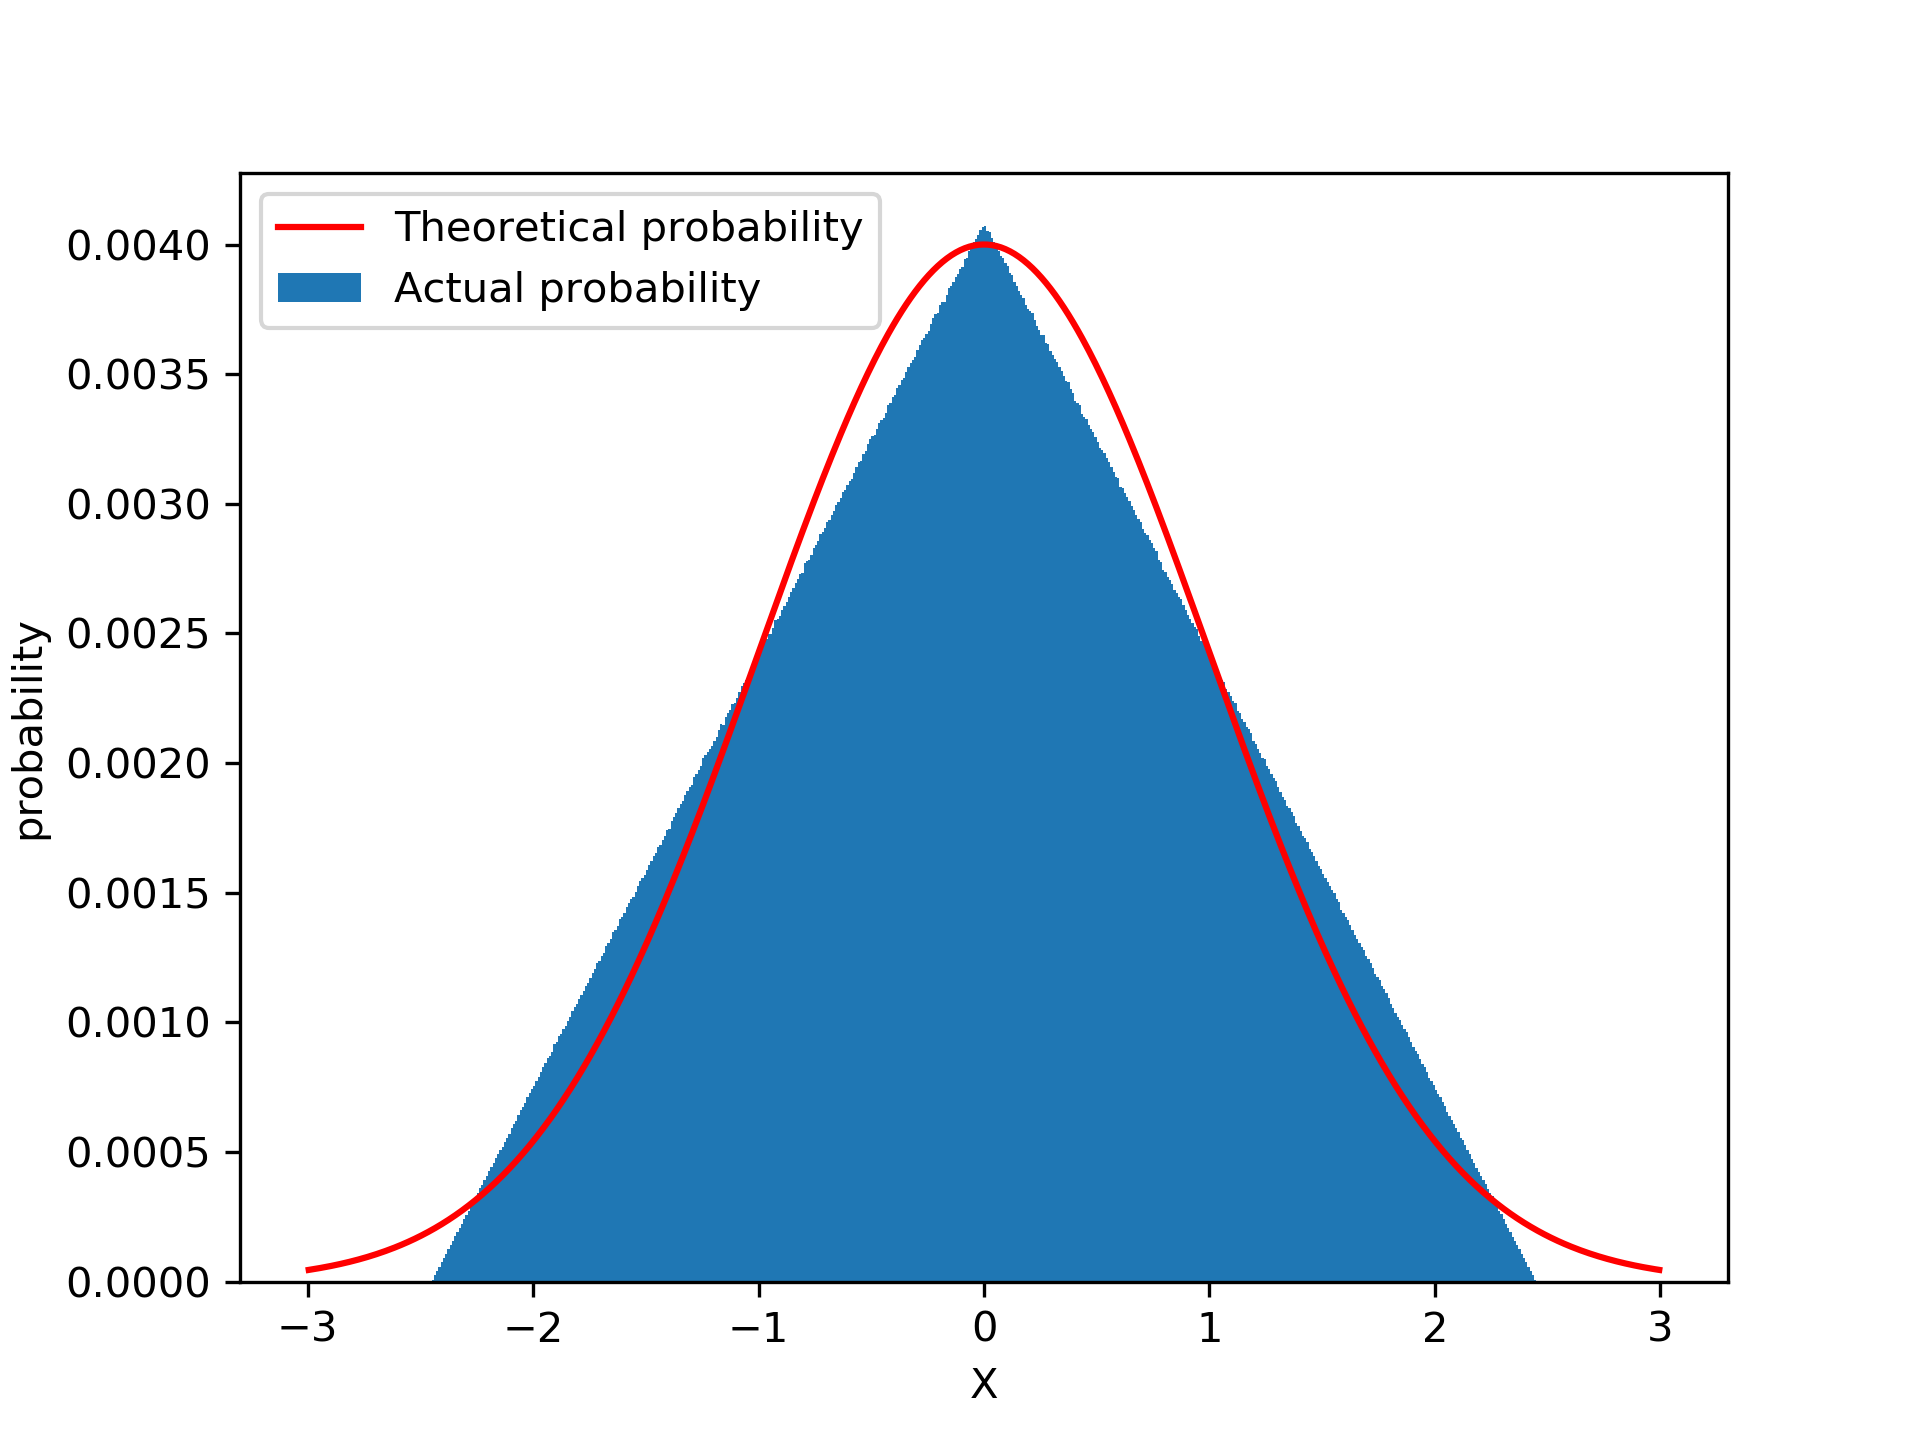
\includegraphics[width=4cm] {2-8-2.png}
}
\subfigure[每次抽样5个点]{
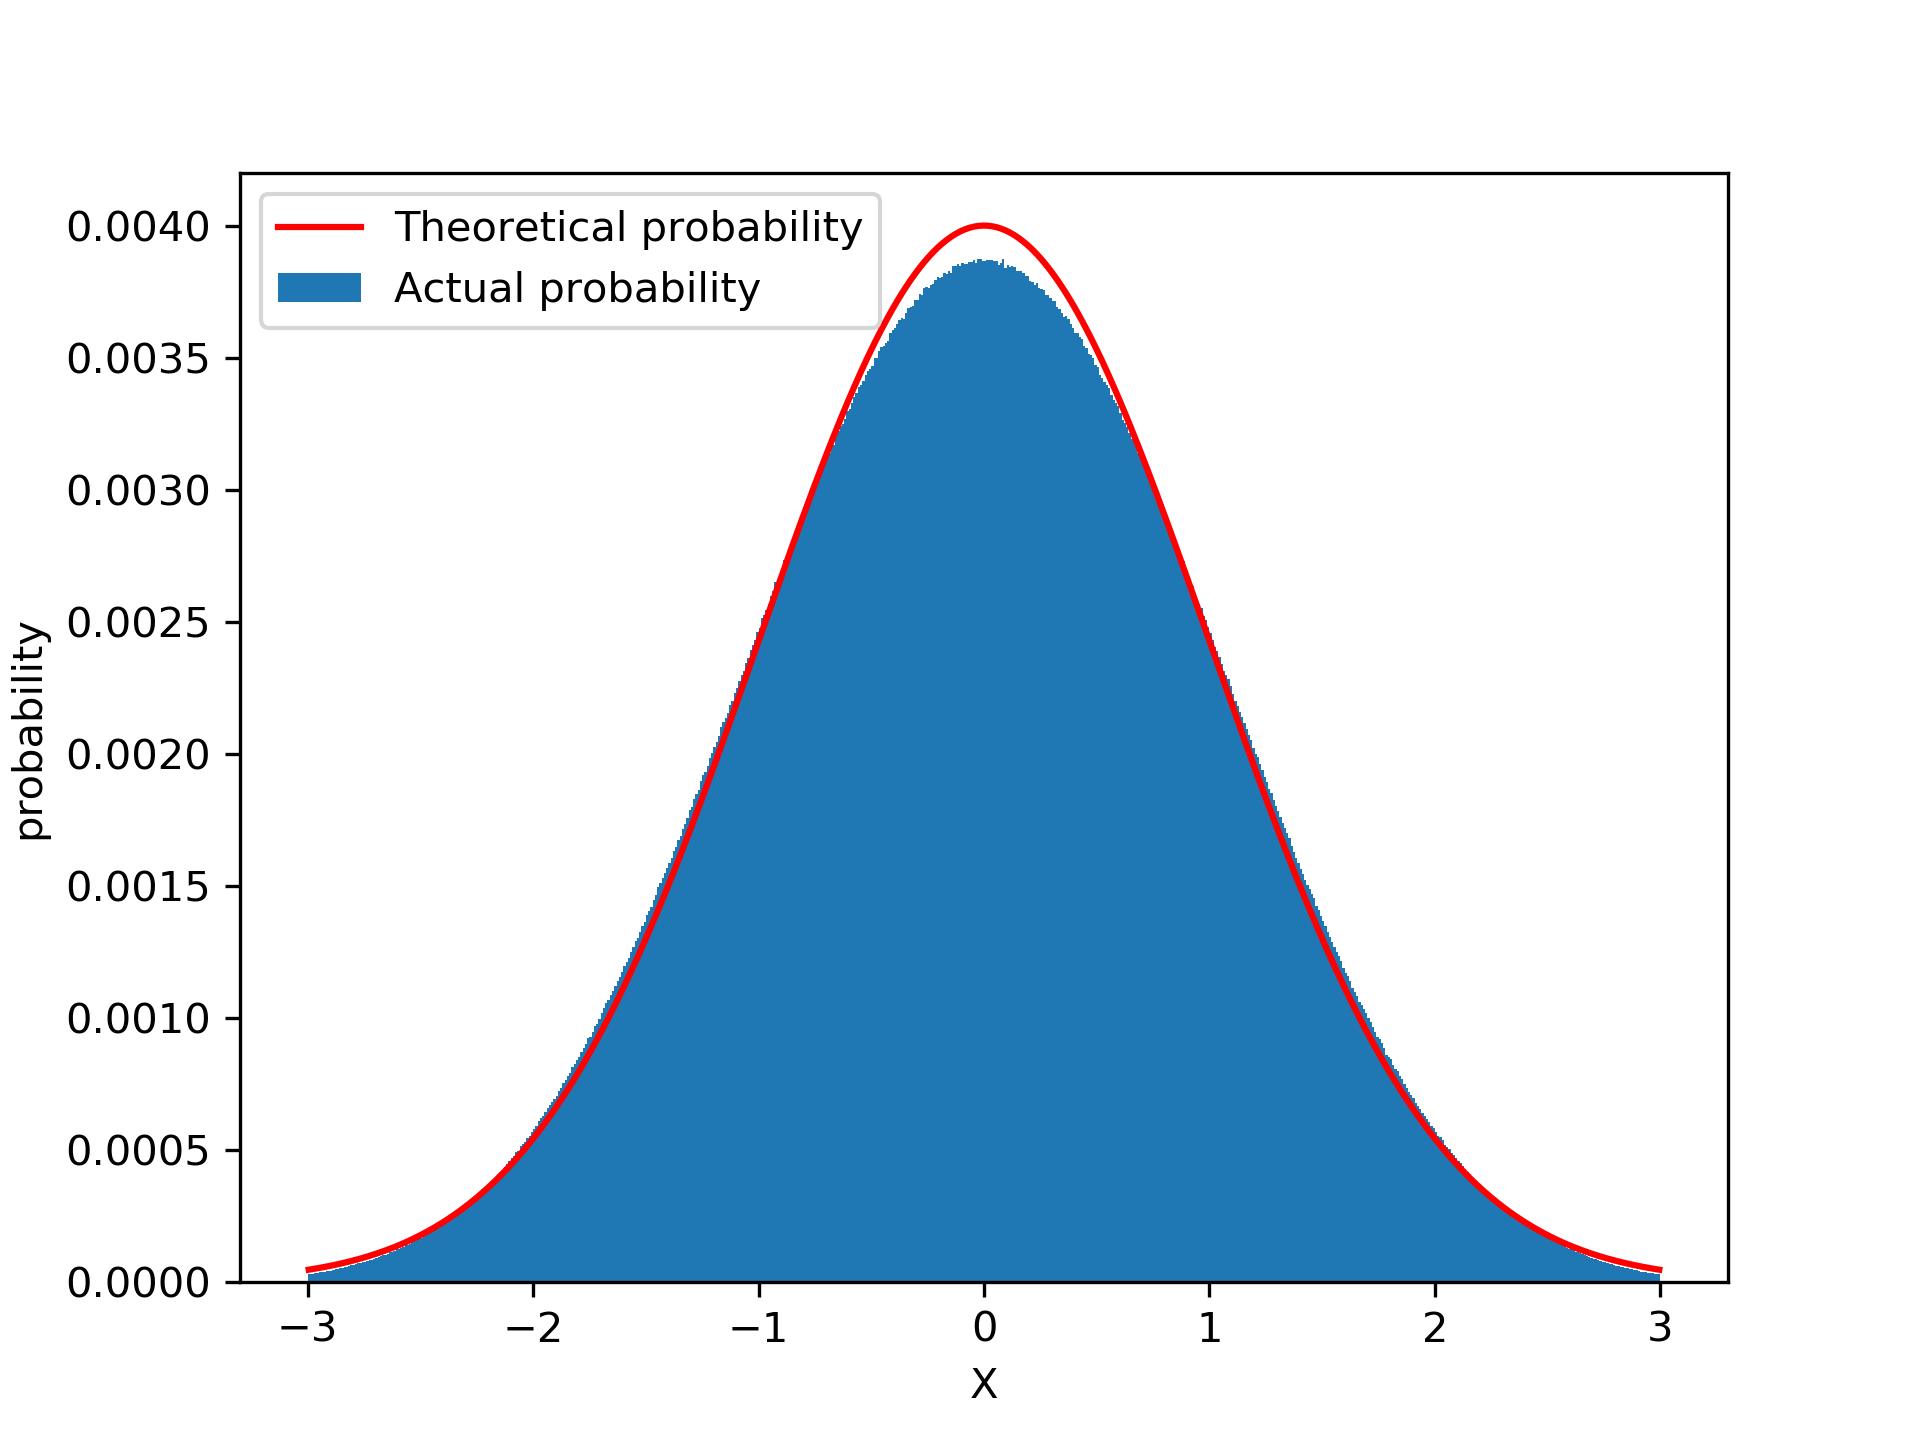
\includegraphics[width=4cm] {2-8-5.png}
}      
\subfigure[每次抽样10个点]{
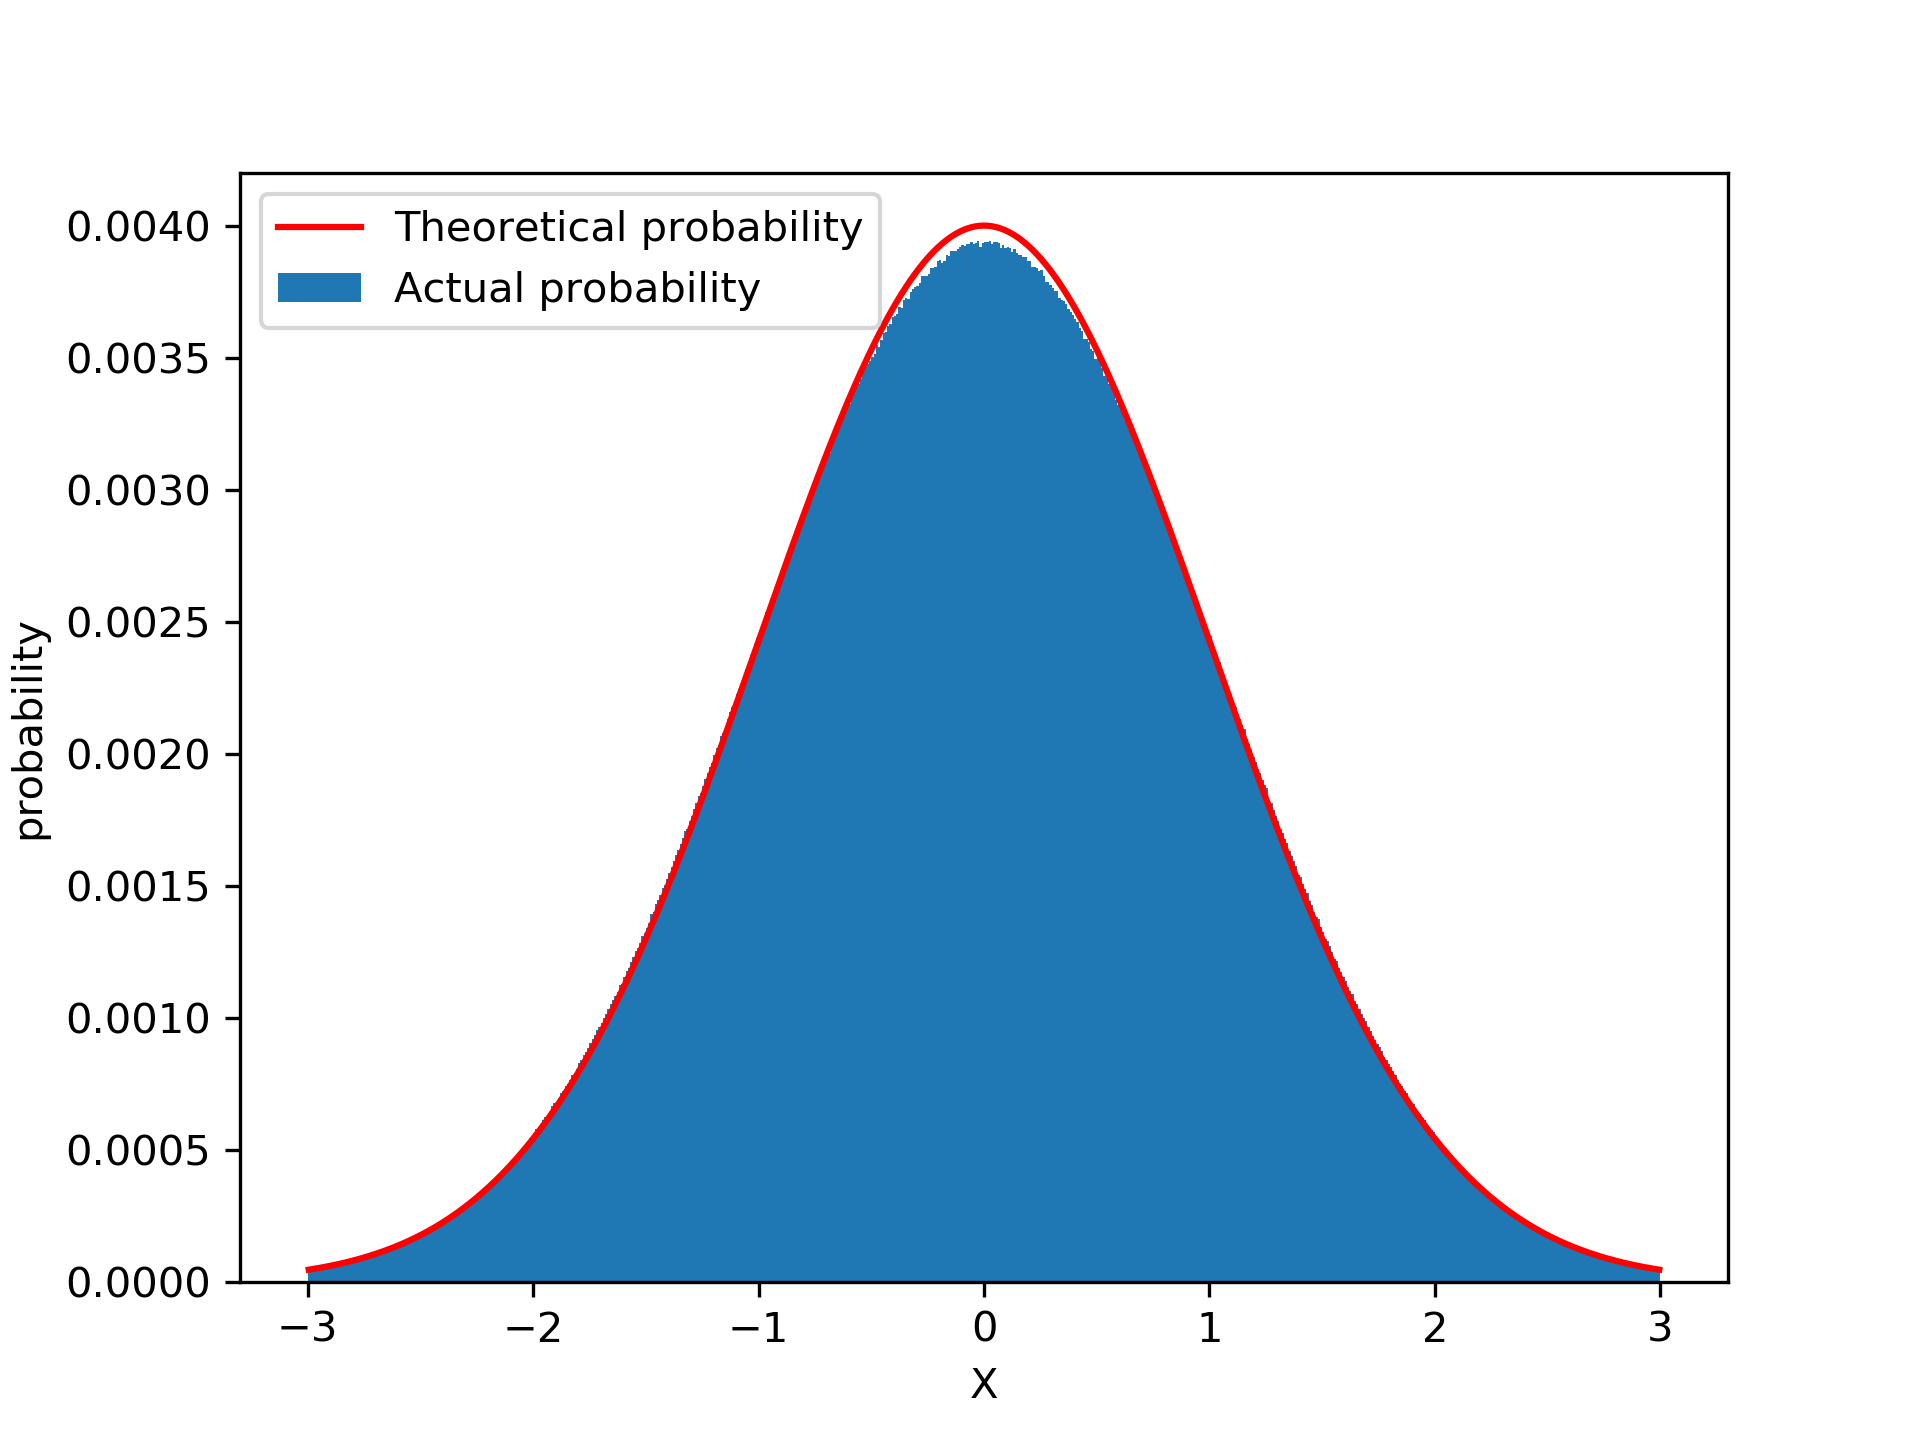
\includegraphics[width=4cm] {2-8-10.png}
}      
\caption{2号分布计算$10^{8}$次后的结果}      
\end{figure}
 
\newpage 可以看出对于2号分布随着计算计算次数和每次抽样个数的增加,其统计量的分布与标准正态分布越来越接近。

\begin{figure}[!htbp]   
\centering     
\subfigure[每次抽样2个点]{
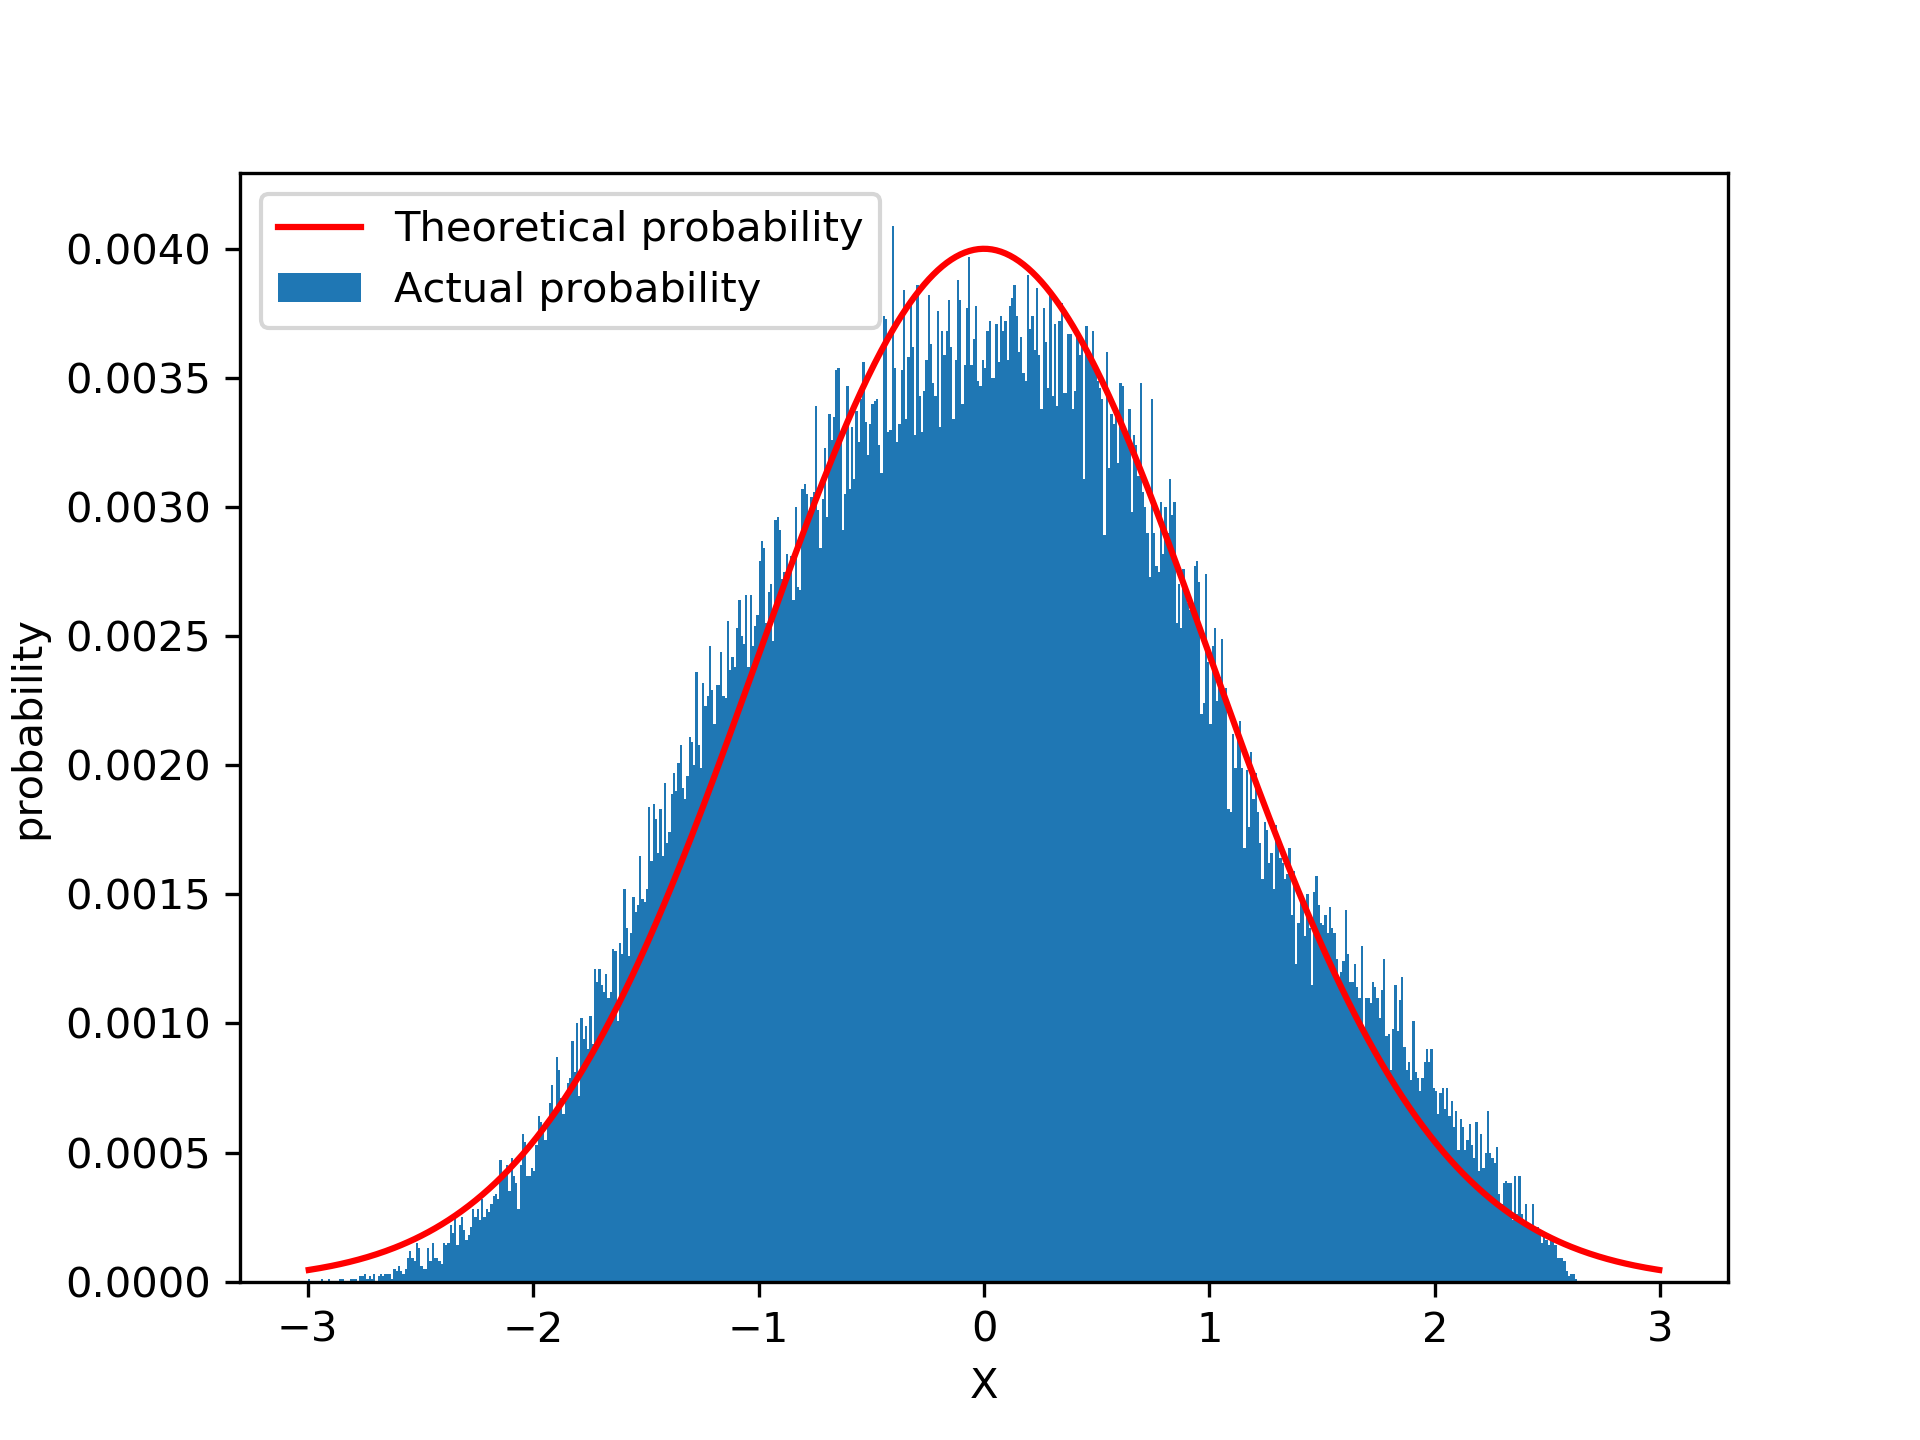
\includegraphics[width=4cm] {3-5-2.png}
}
\subfigure[每次抽样5个点]{
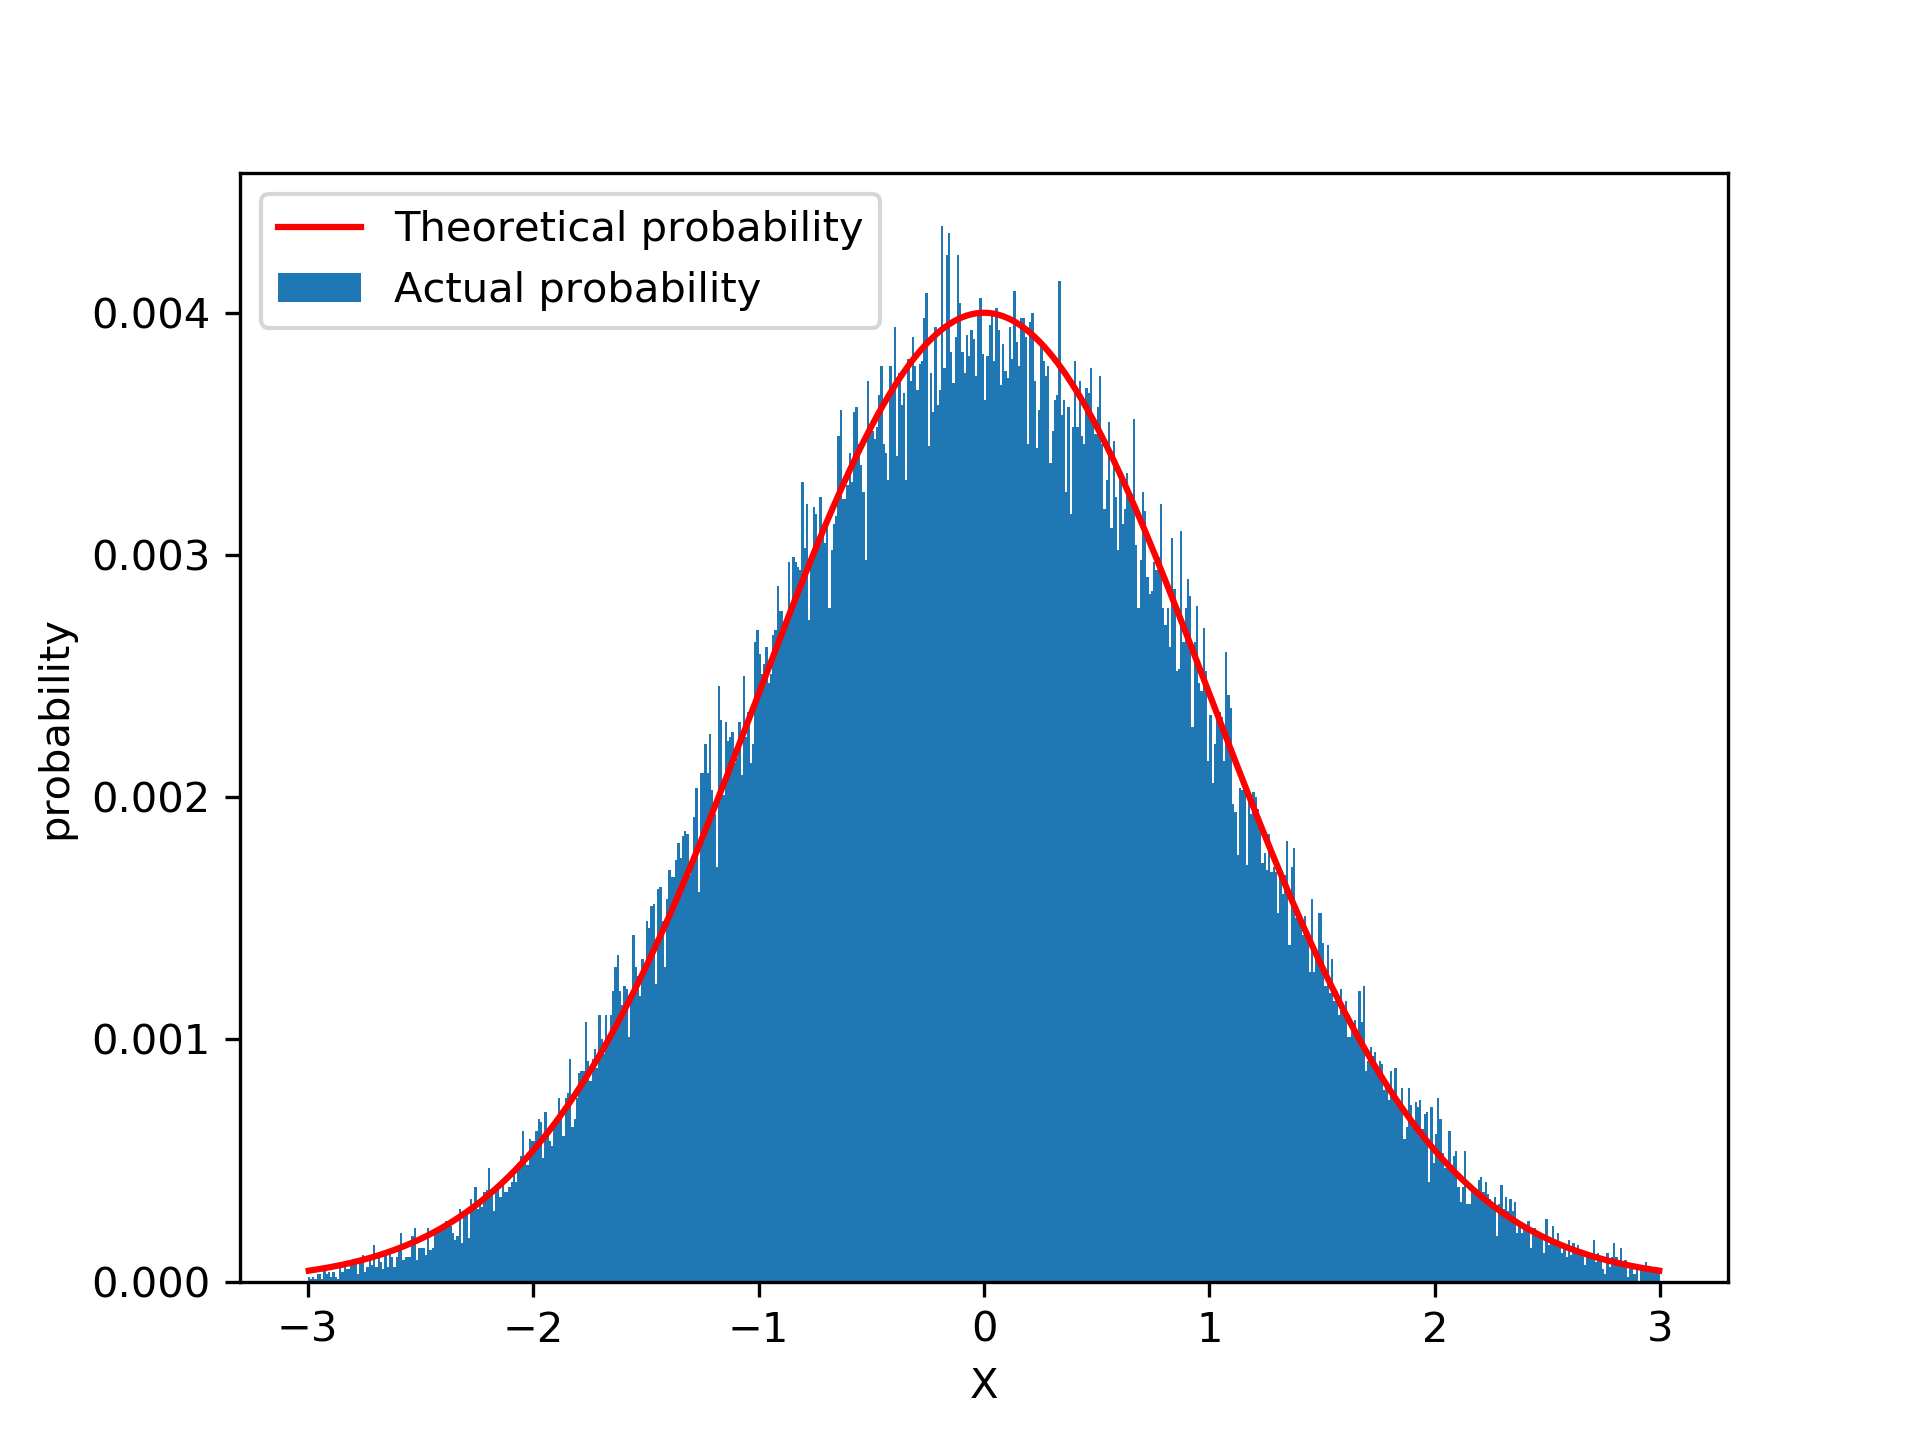
\includegraphics[width=4cm] {3-5-5.png}
}      
\subfigure[每次抽样10个点]{
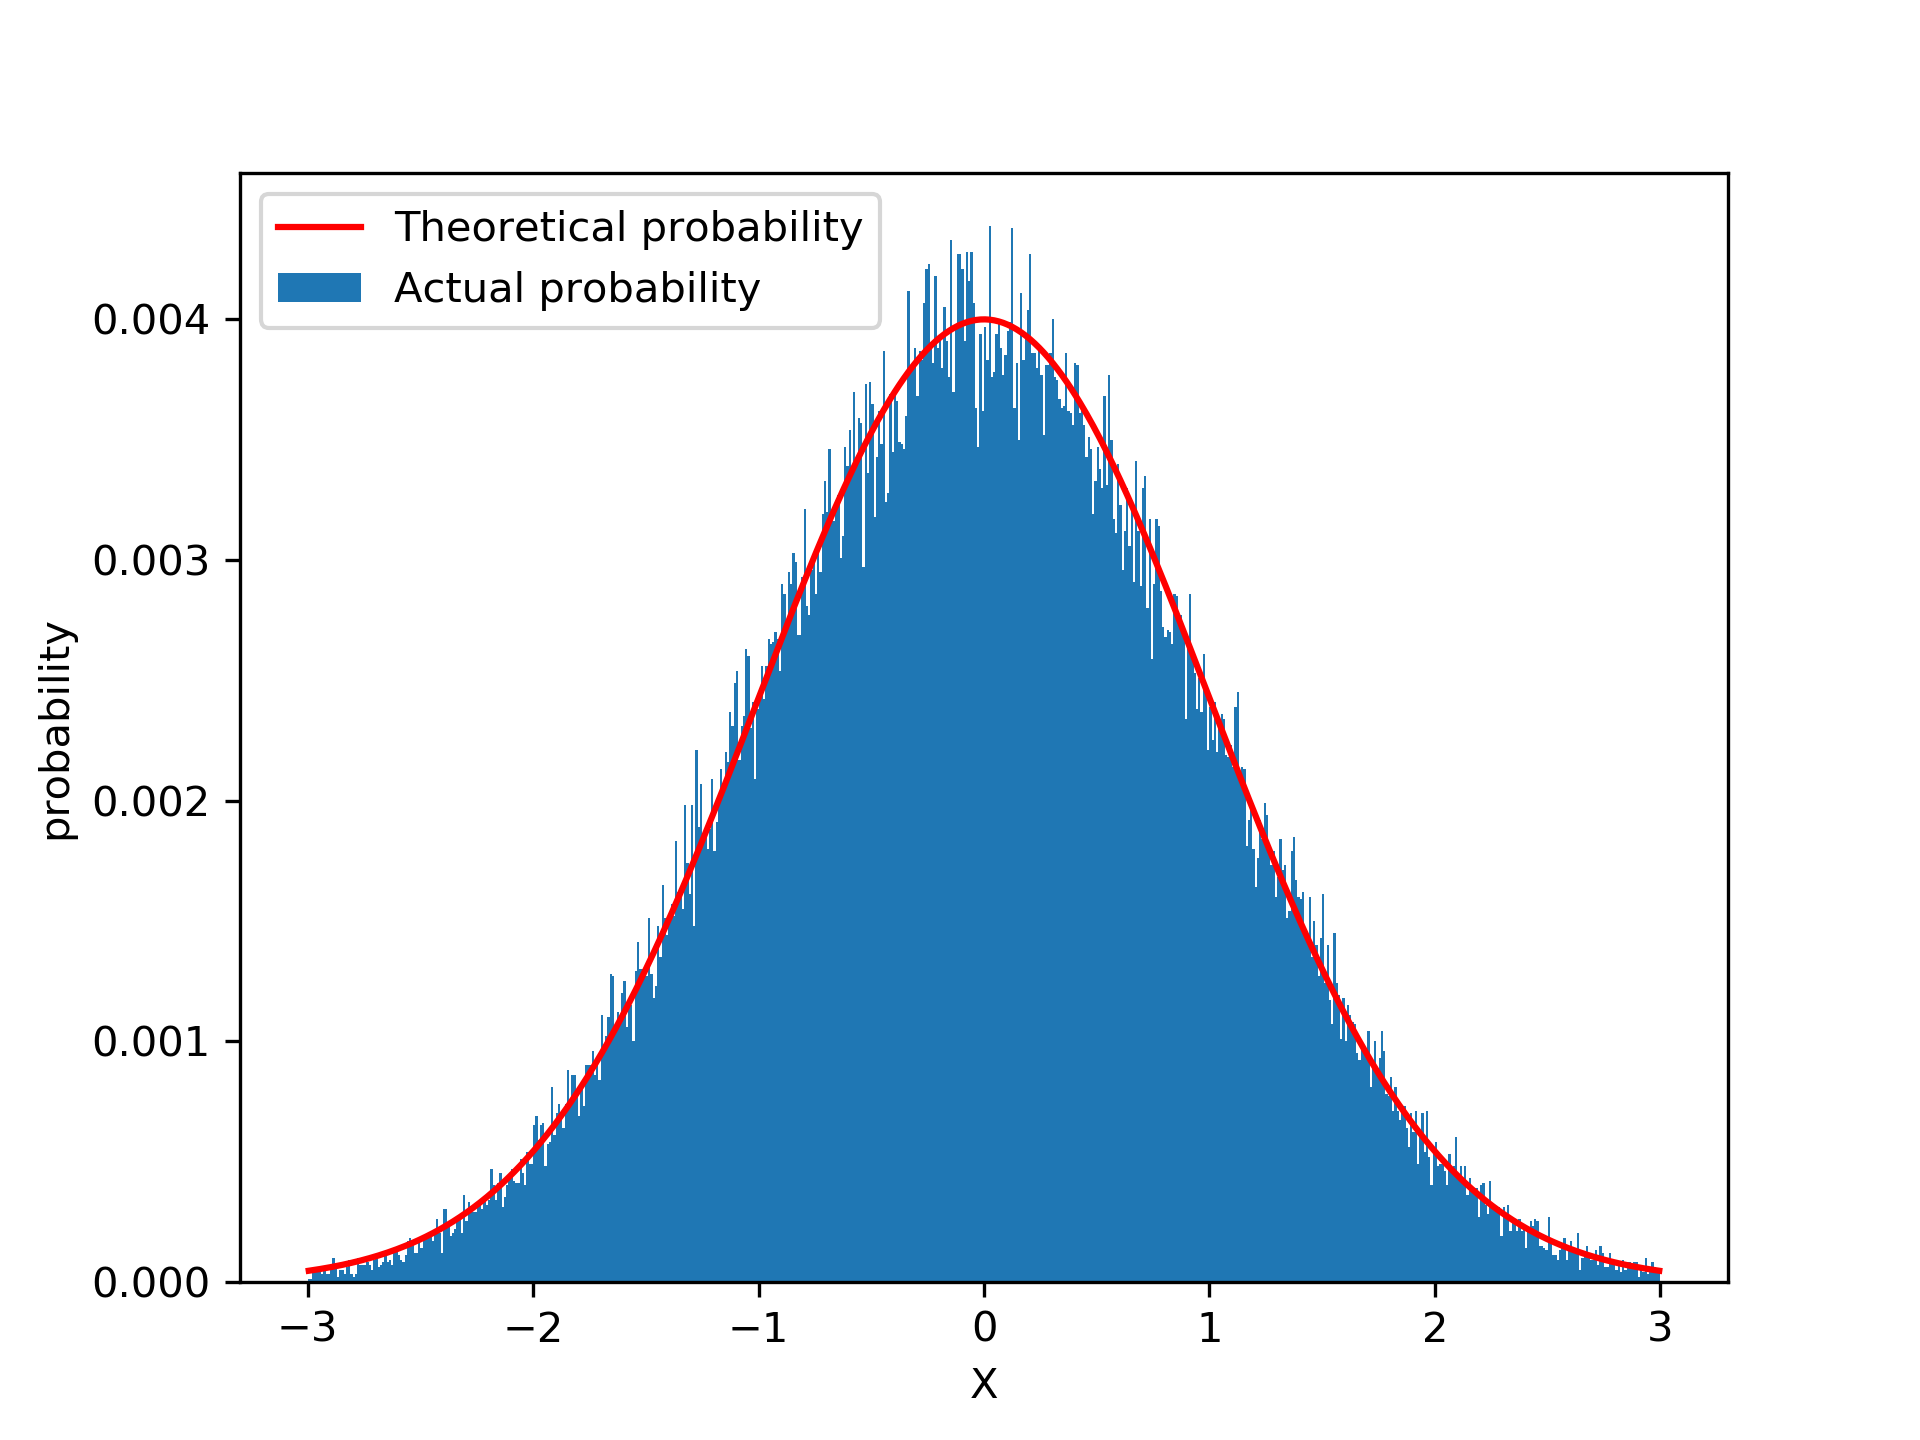
\includegraphics[width=4cm] {3-5-10.png}
}      
\caption{3号分布计算$10^{5}$次后的结果}      
\end{figure}


\begin{figure}[!htbp]   
\centering     
\subfigure[每次抽样2个点]{
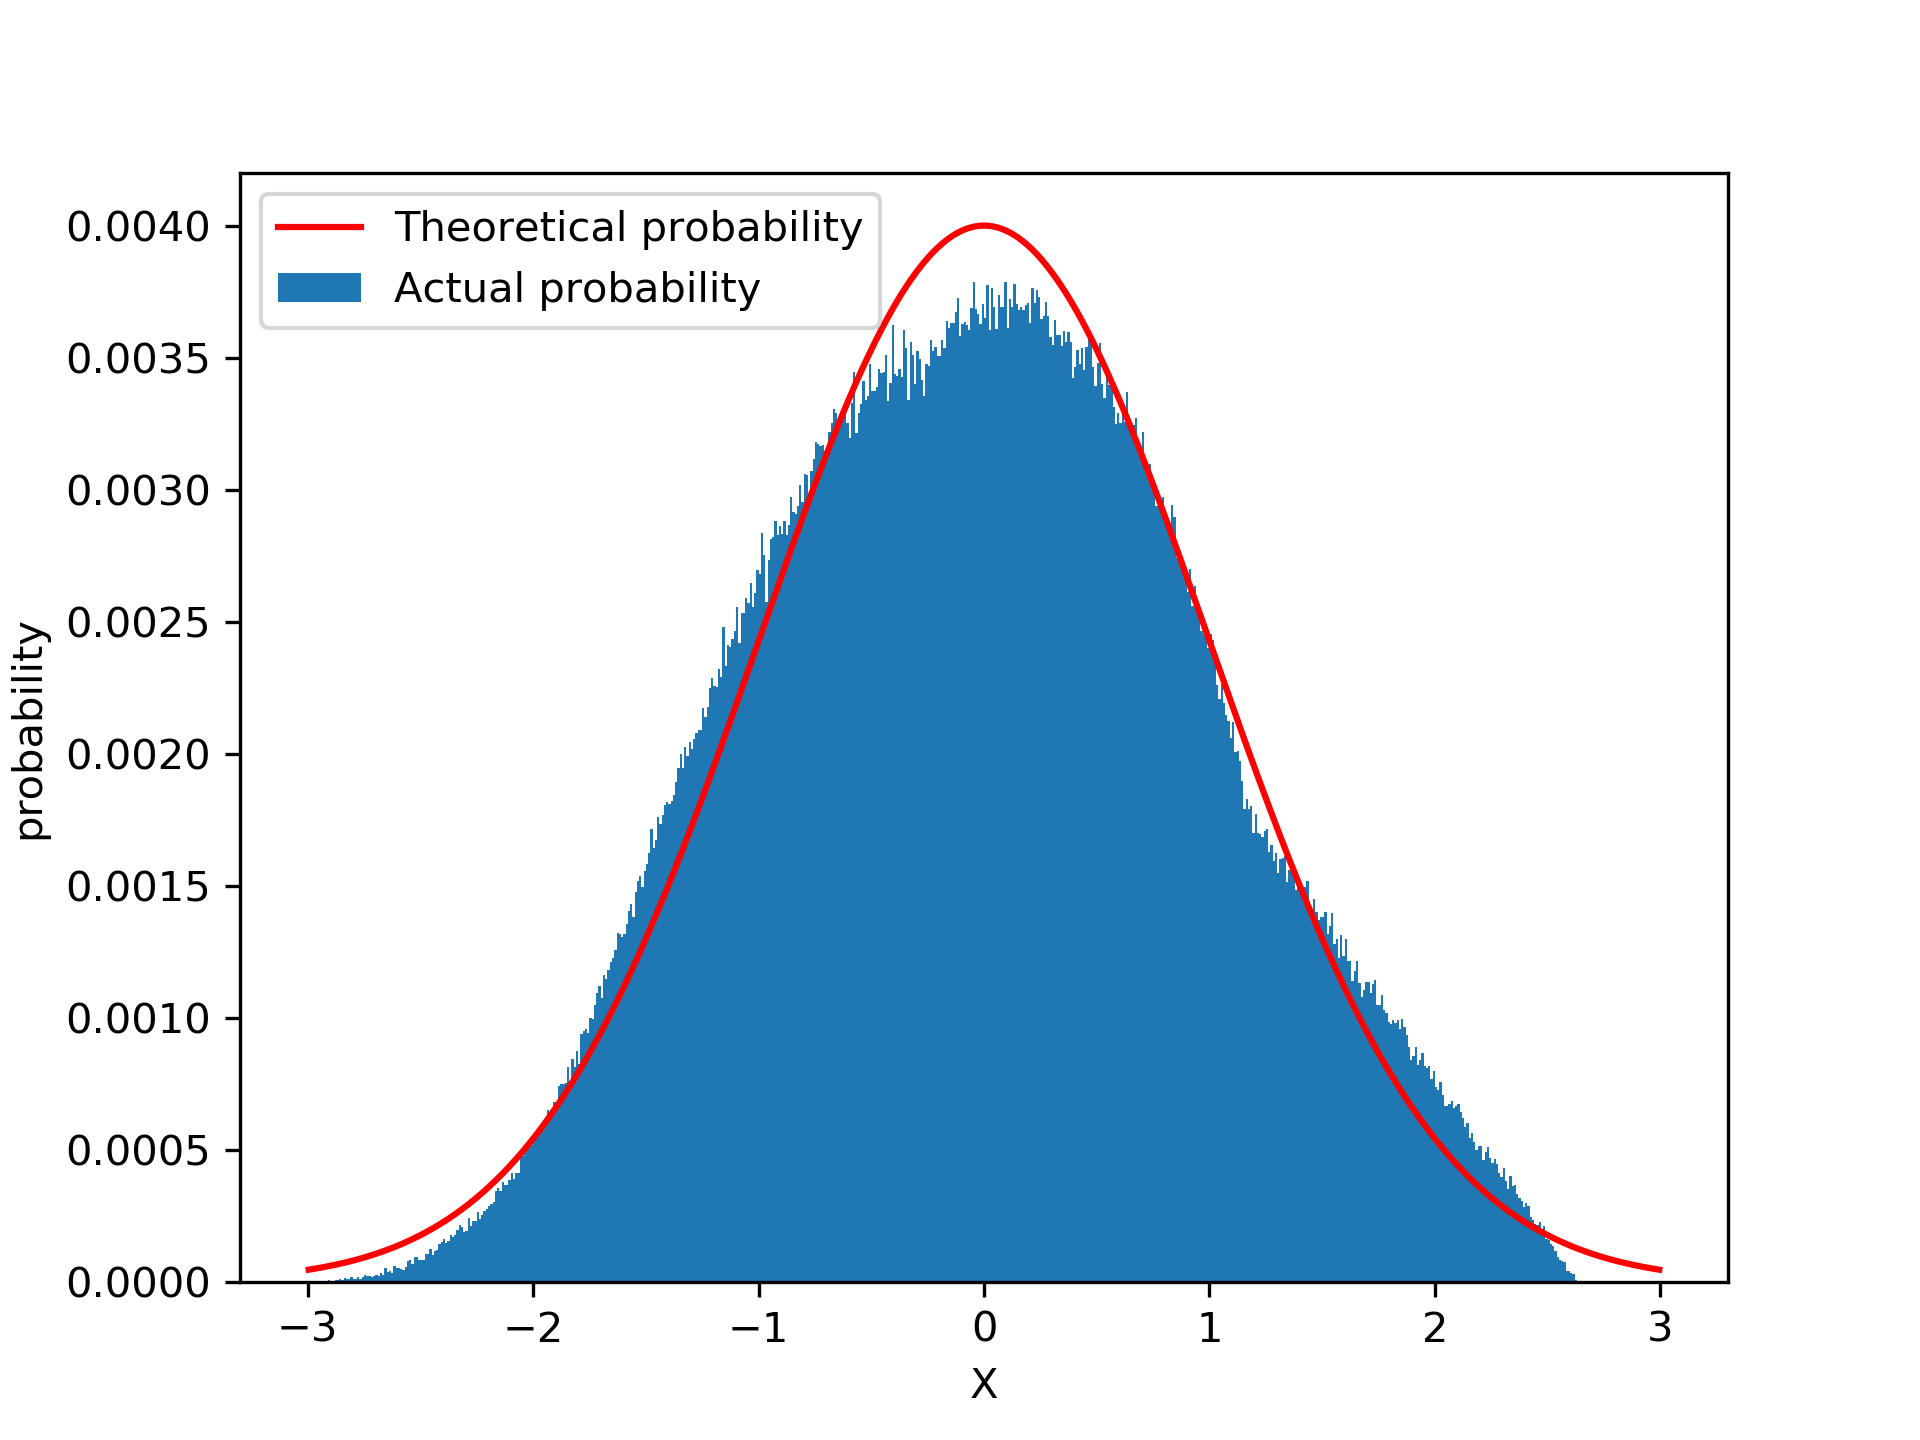
\includegraphics[width=4cm] {3-6-2.png}
}
\subfigure[每次抽样5个点]{
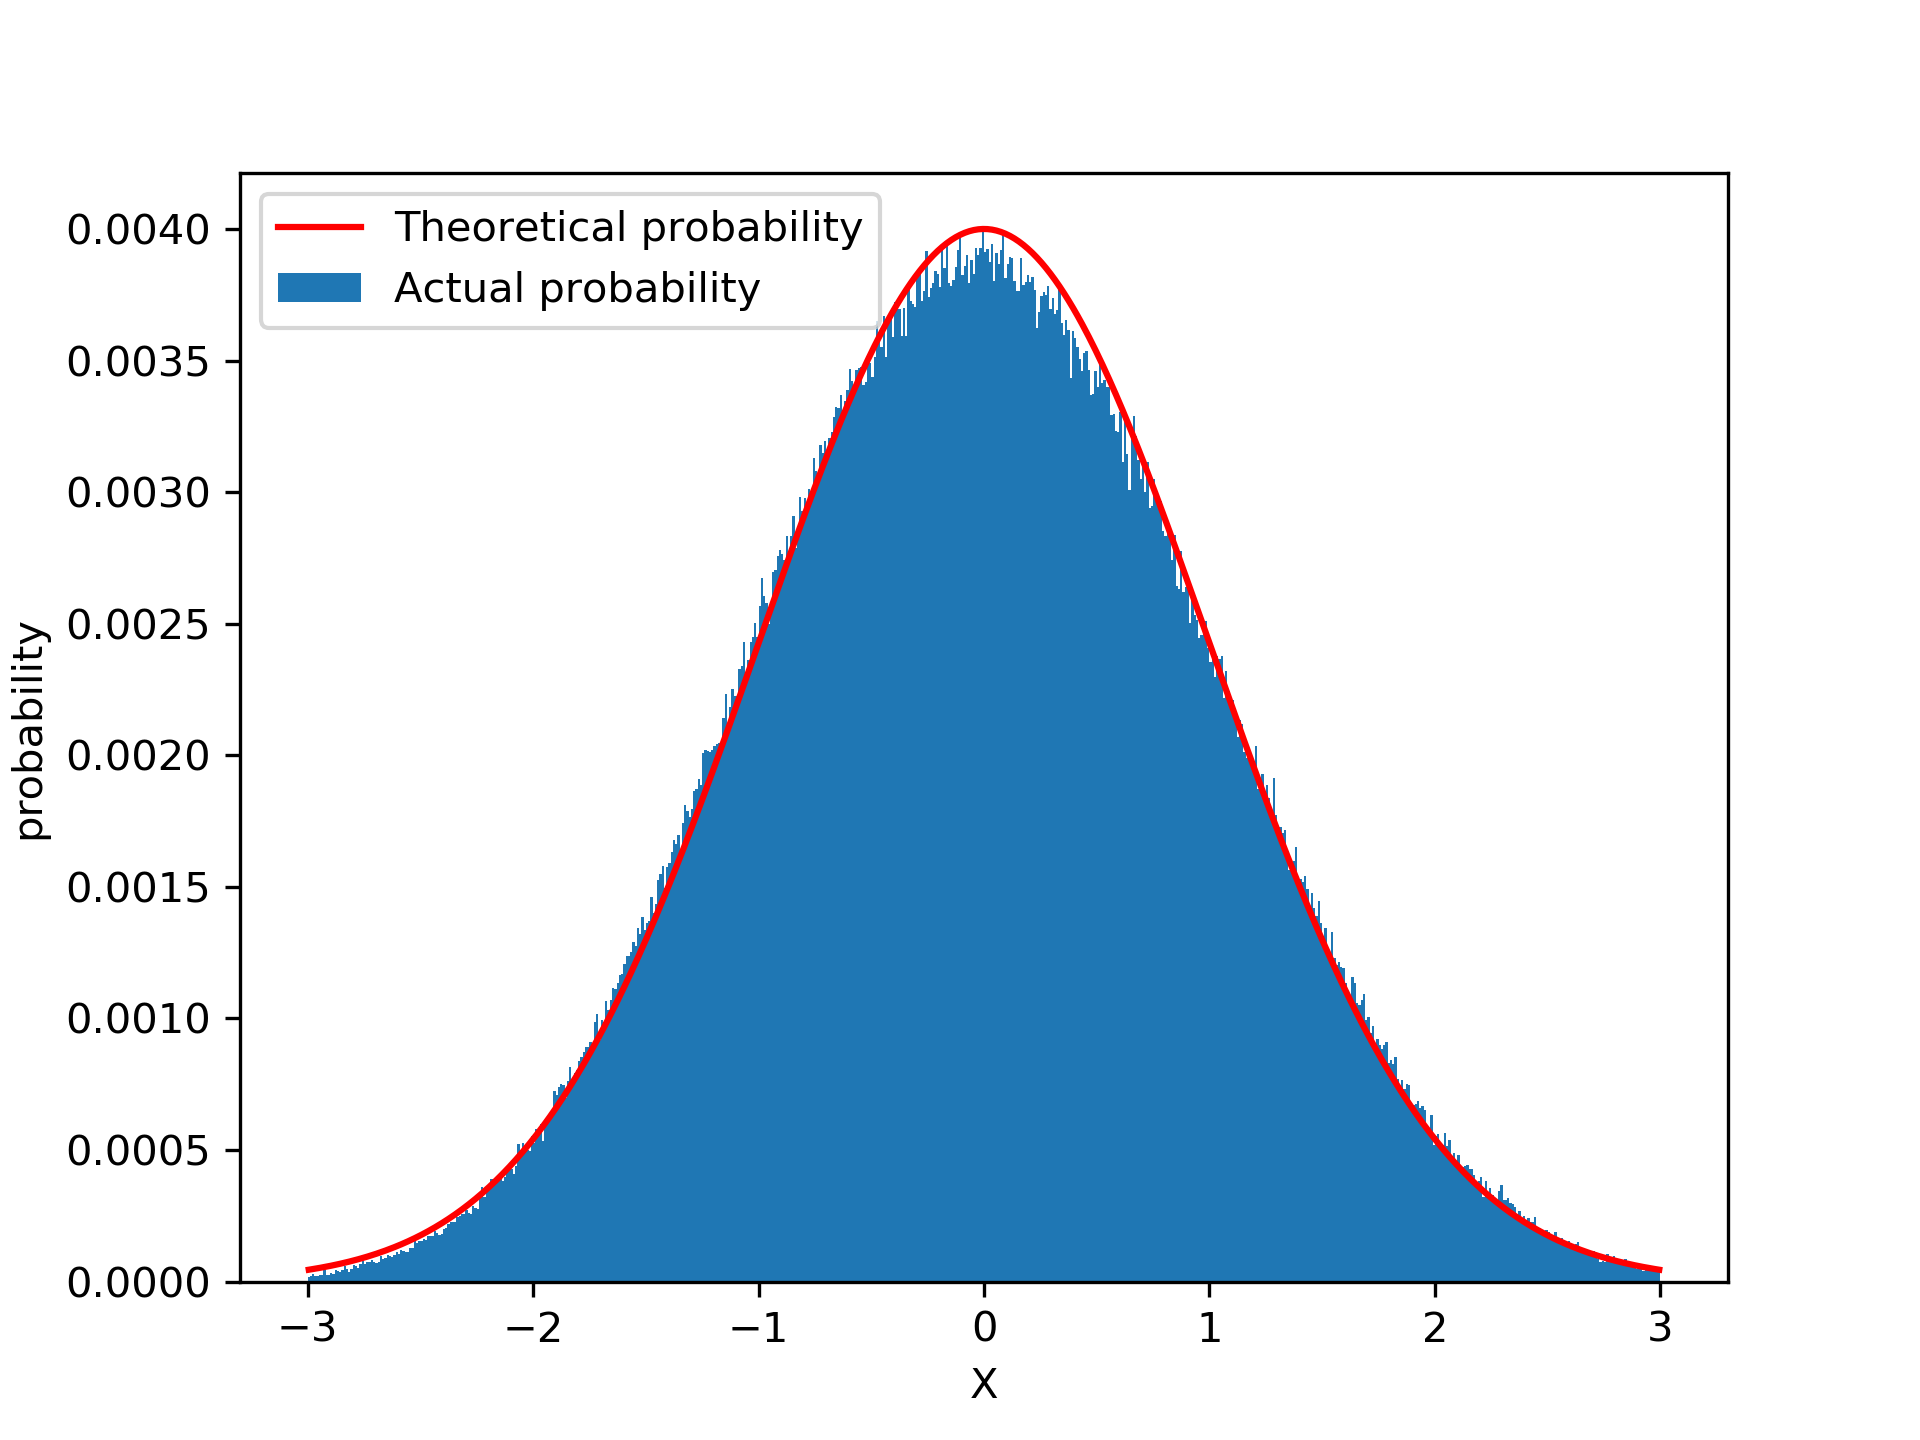
\includegraphics[width=4cm] {3-6-5.png}
}      
\subfigure[每次抽样10个点]{
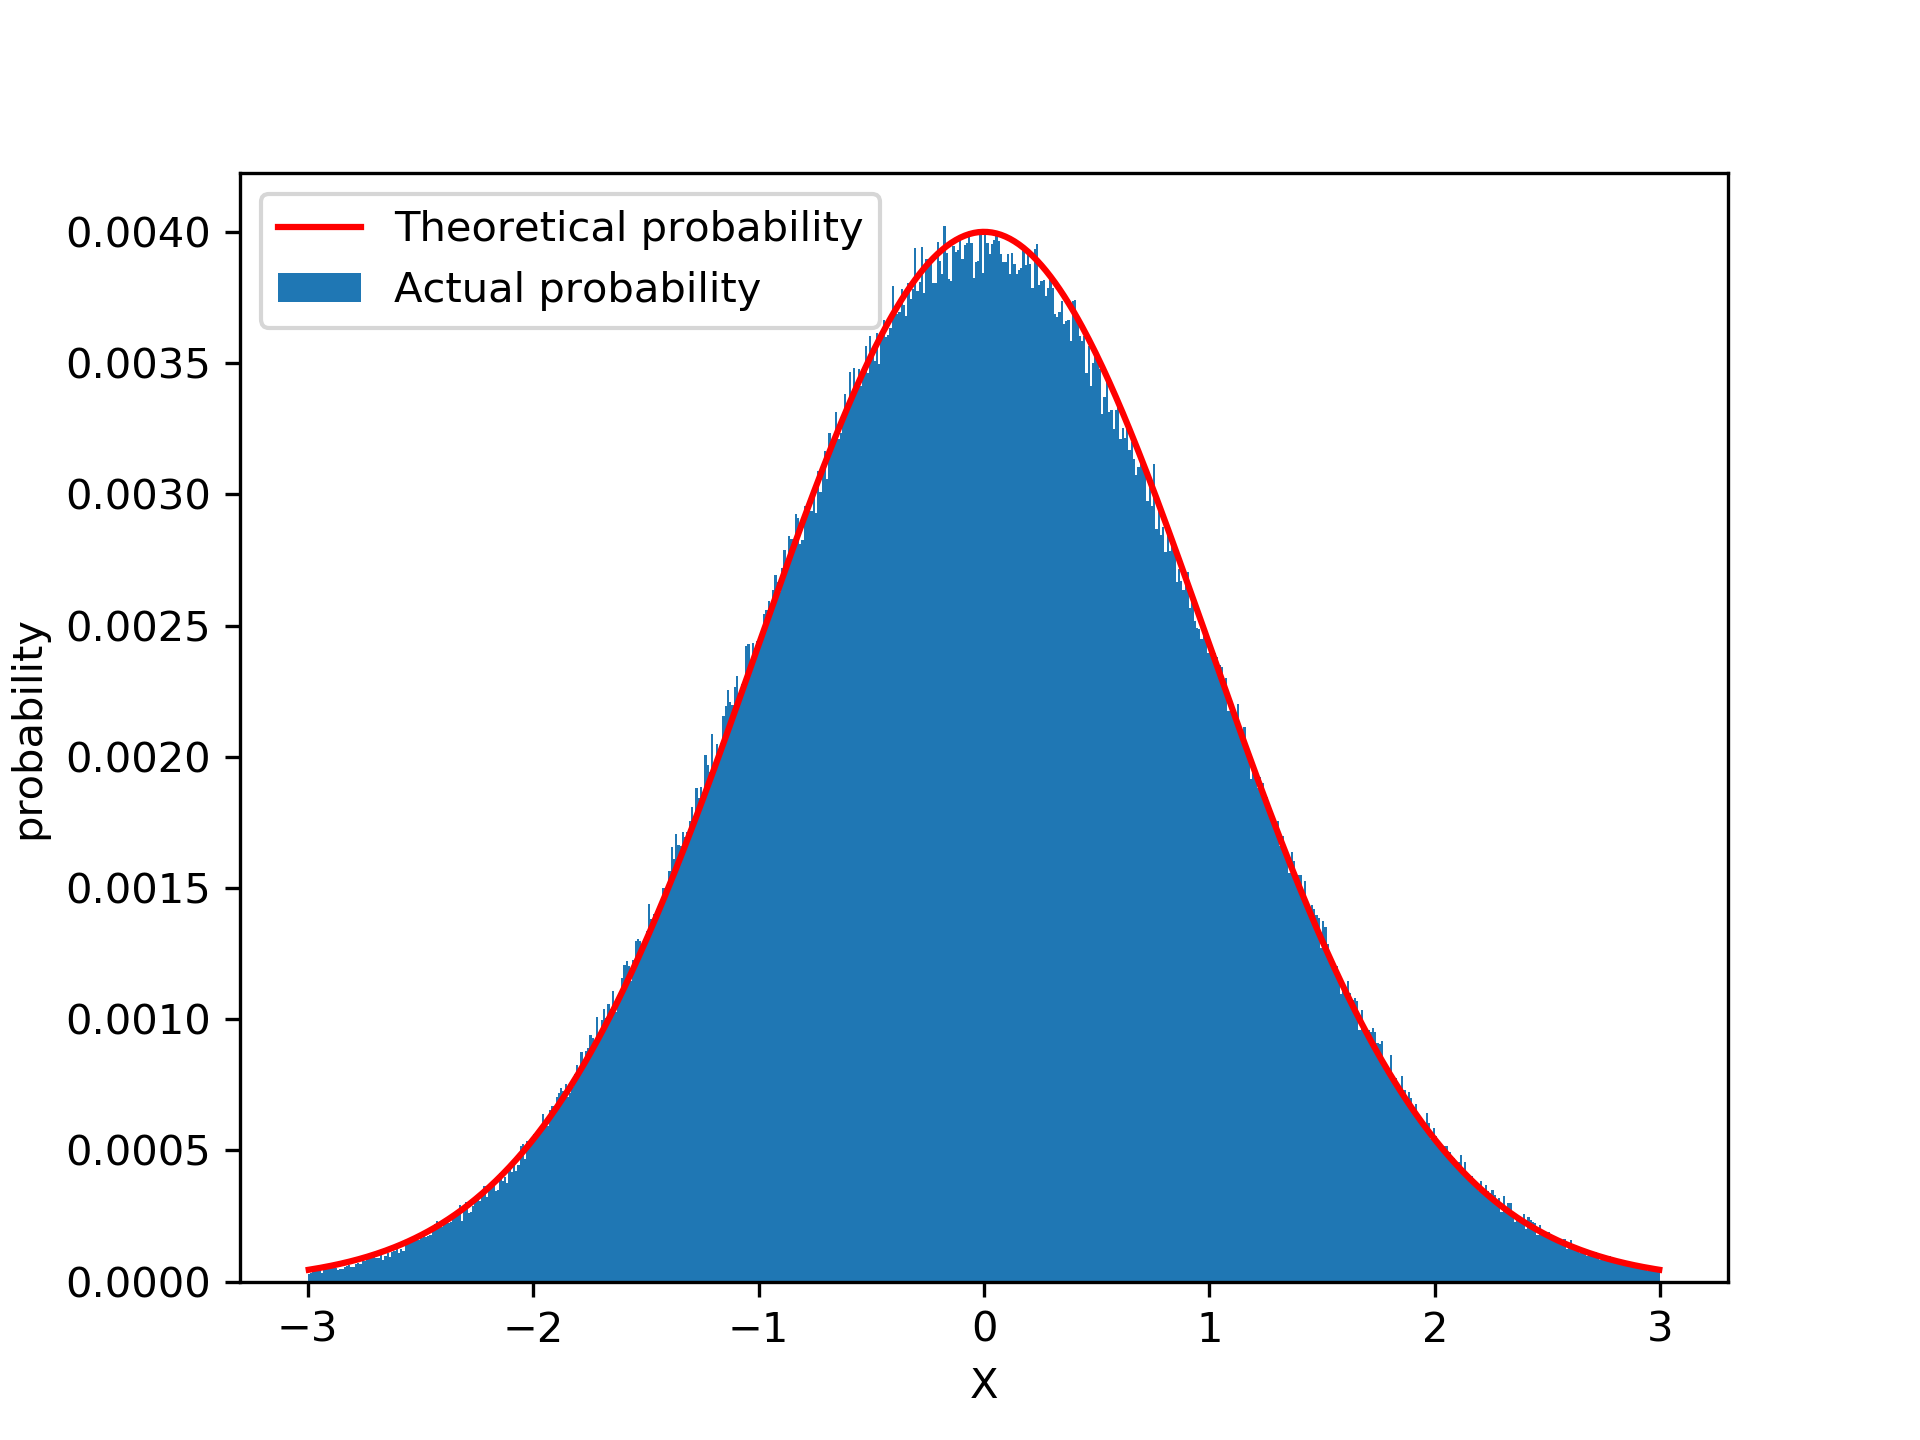
\includegraphics[width=4cm] {3-6-10.png}
}      
\caption{3号分布计算$10^{6}$次后的结果}      
\end{figure}


\begin{figure}[!htbp]   
\centering     
\subfigure[每次抽样2个点]{
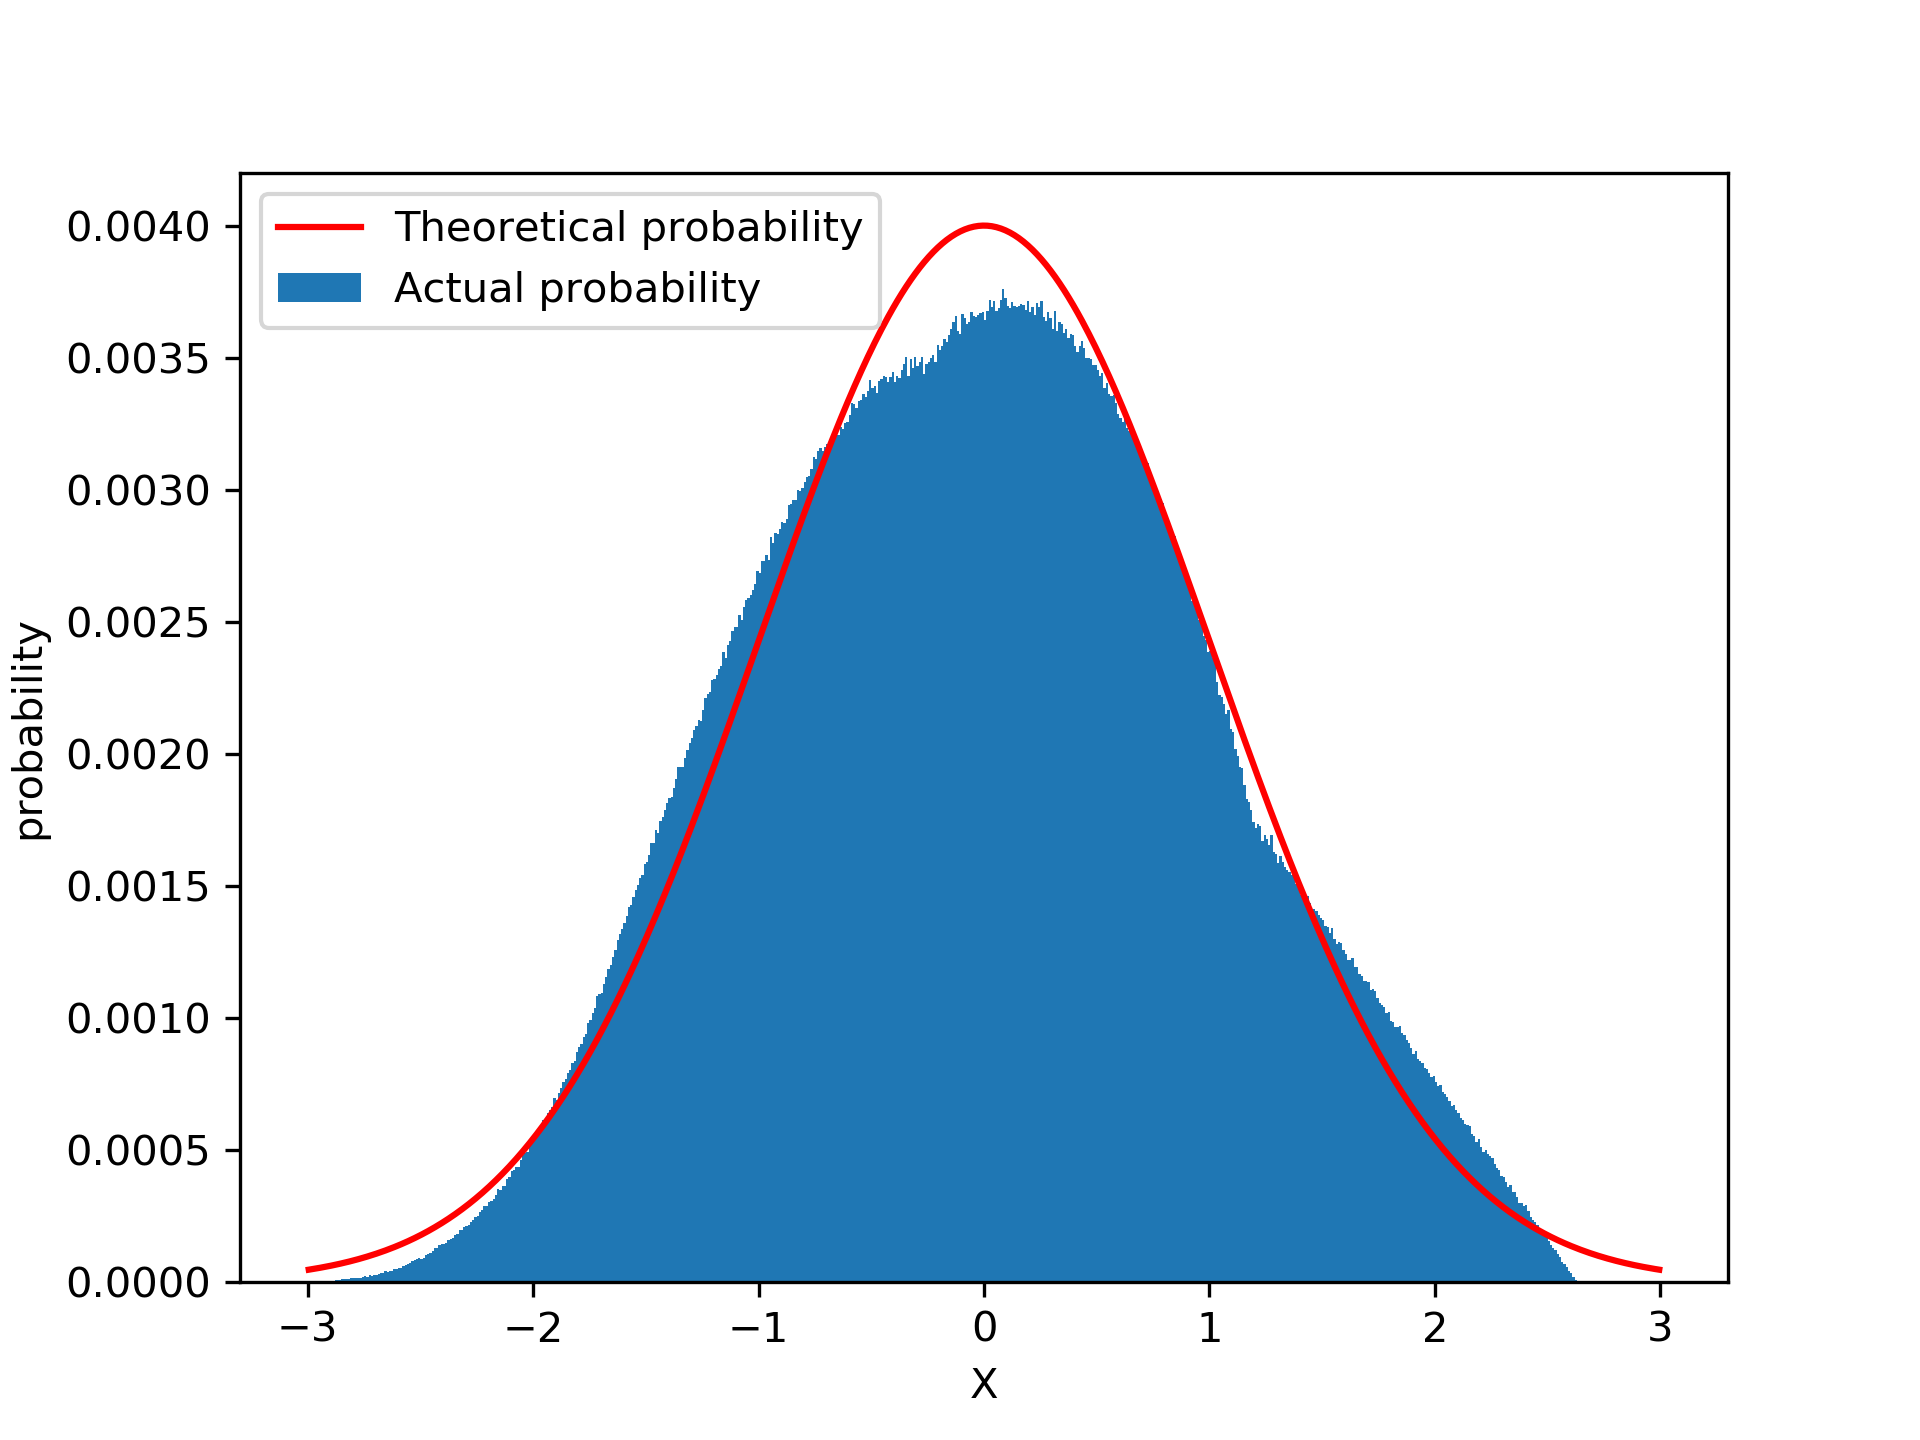
\includegraphics[width=4cm] {3-7-2.png}
}
\subfigure[每次抽样5个点]{
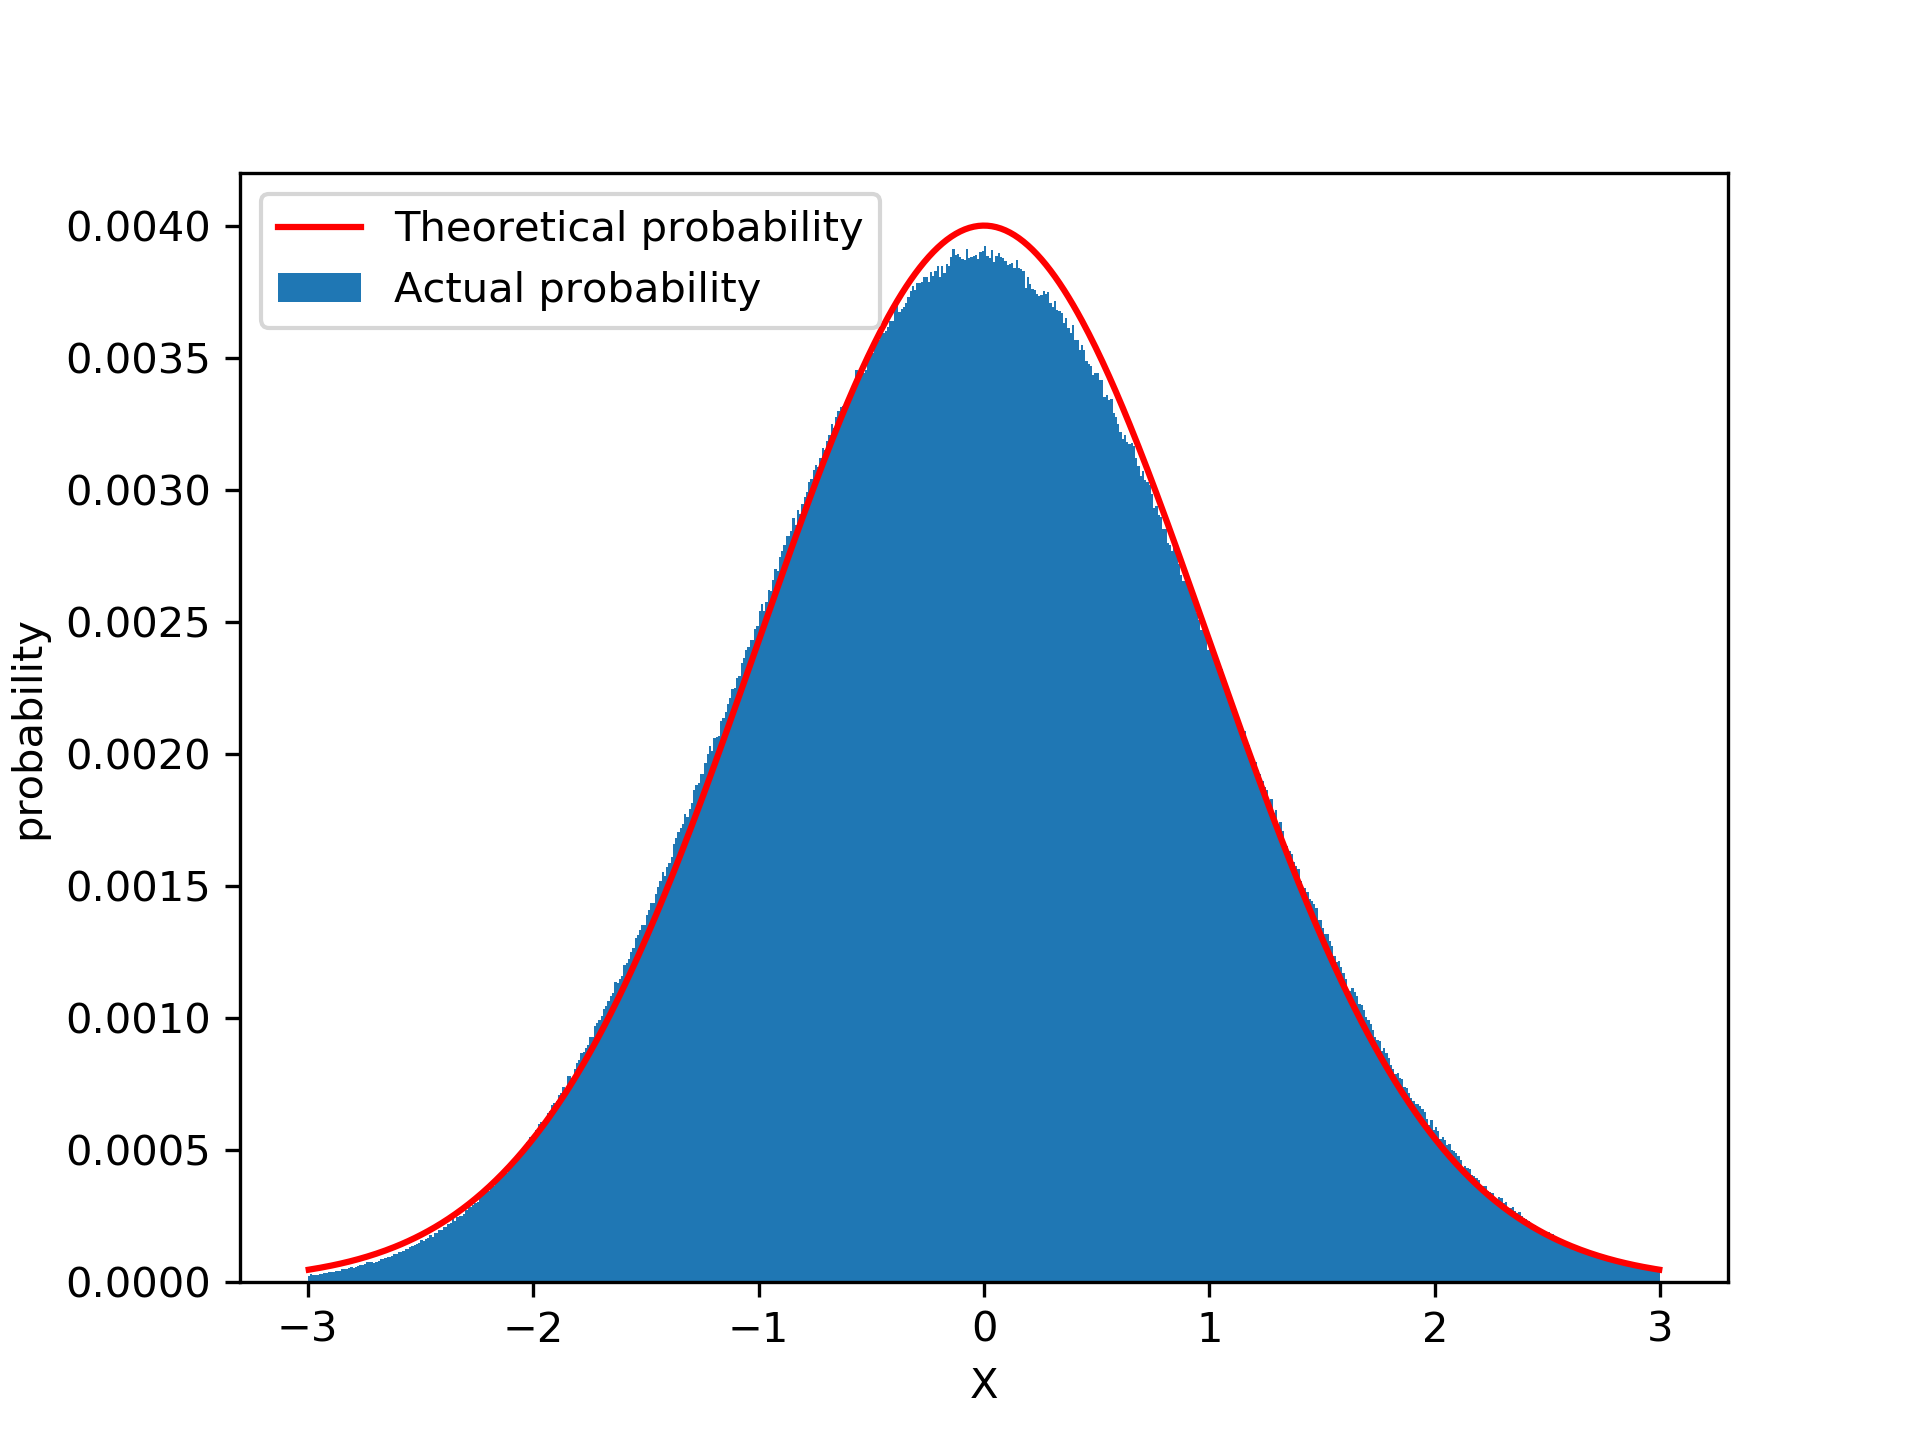
\includegraphics[width=4cm] {3-7-5.png}
}      
\subfigure[每次抽样10个点]{
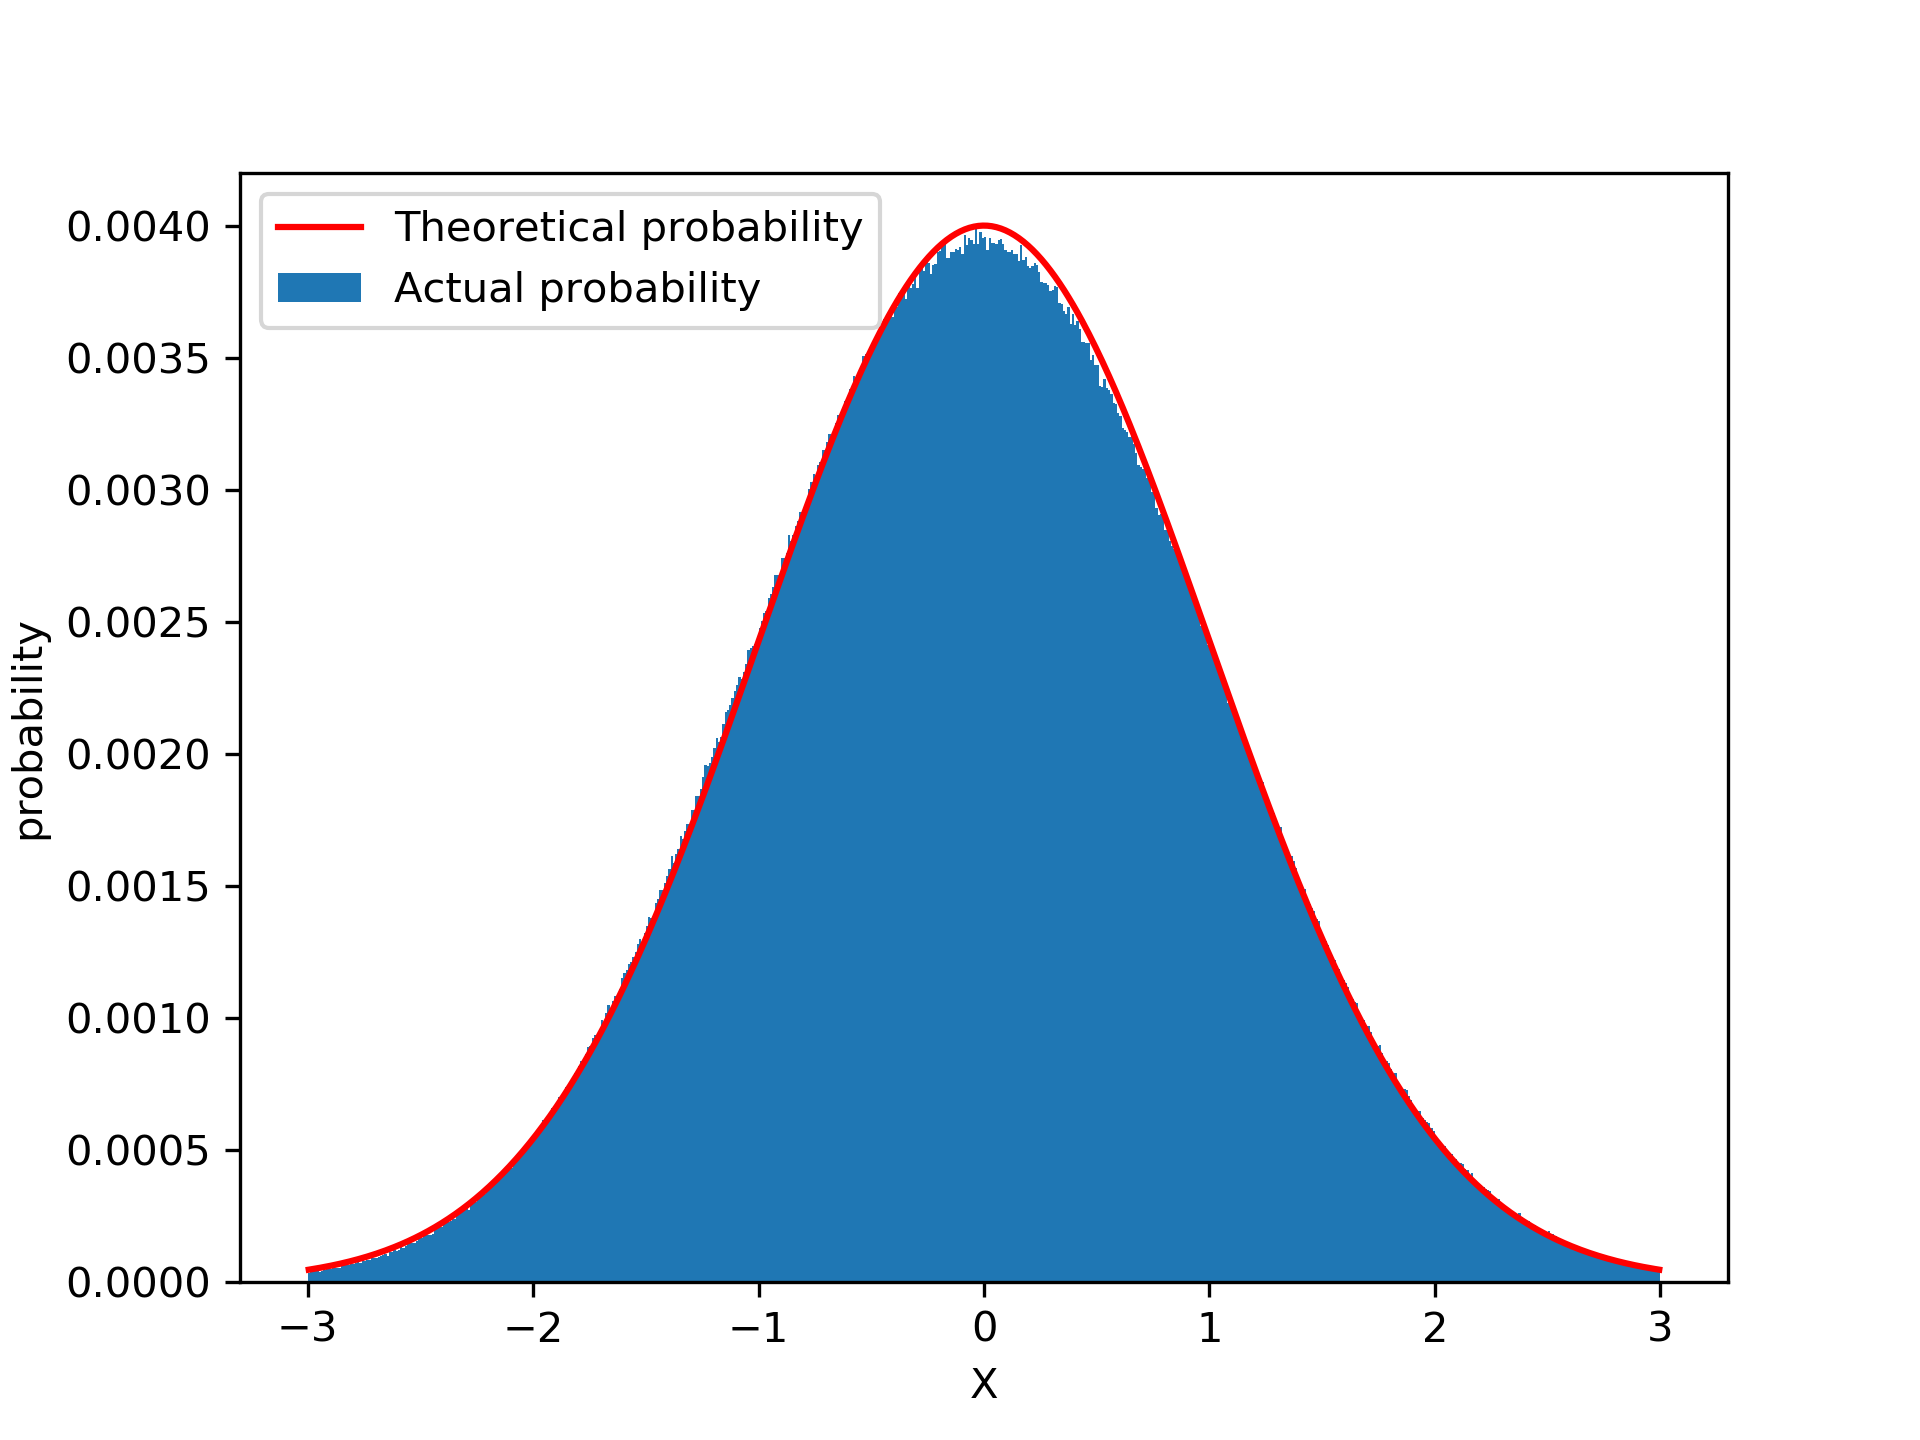
\includegraphics[width=4cm] {3-7-10.png}
}      
\caption{3号分布计算$10^{7}$次后的结果}     
\end{figure}


\begin{figure}[!htbp]   
\centering     
\subfigure[每次抽样2个点]{
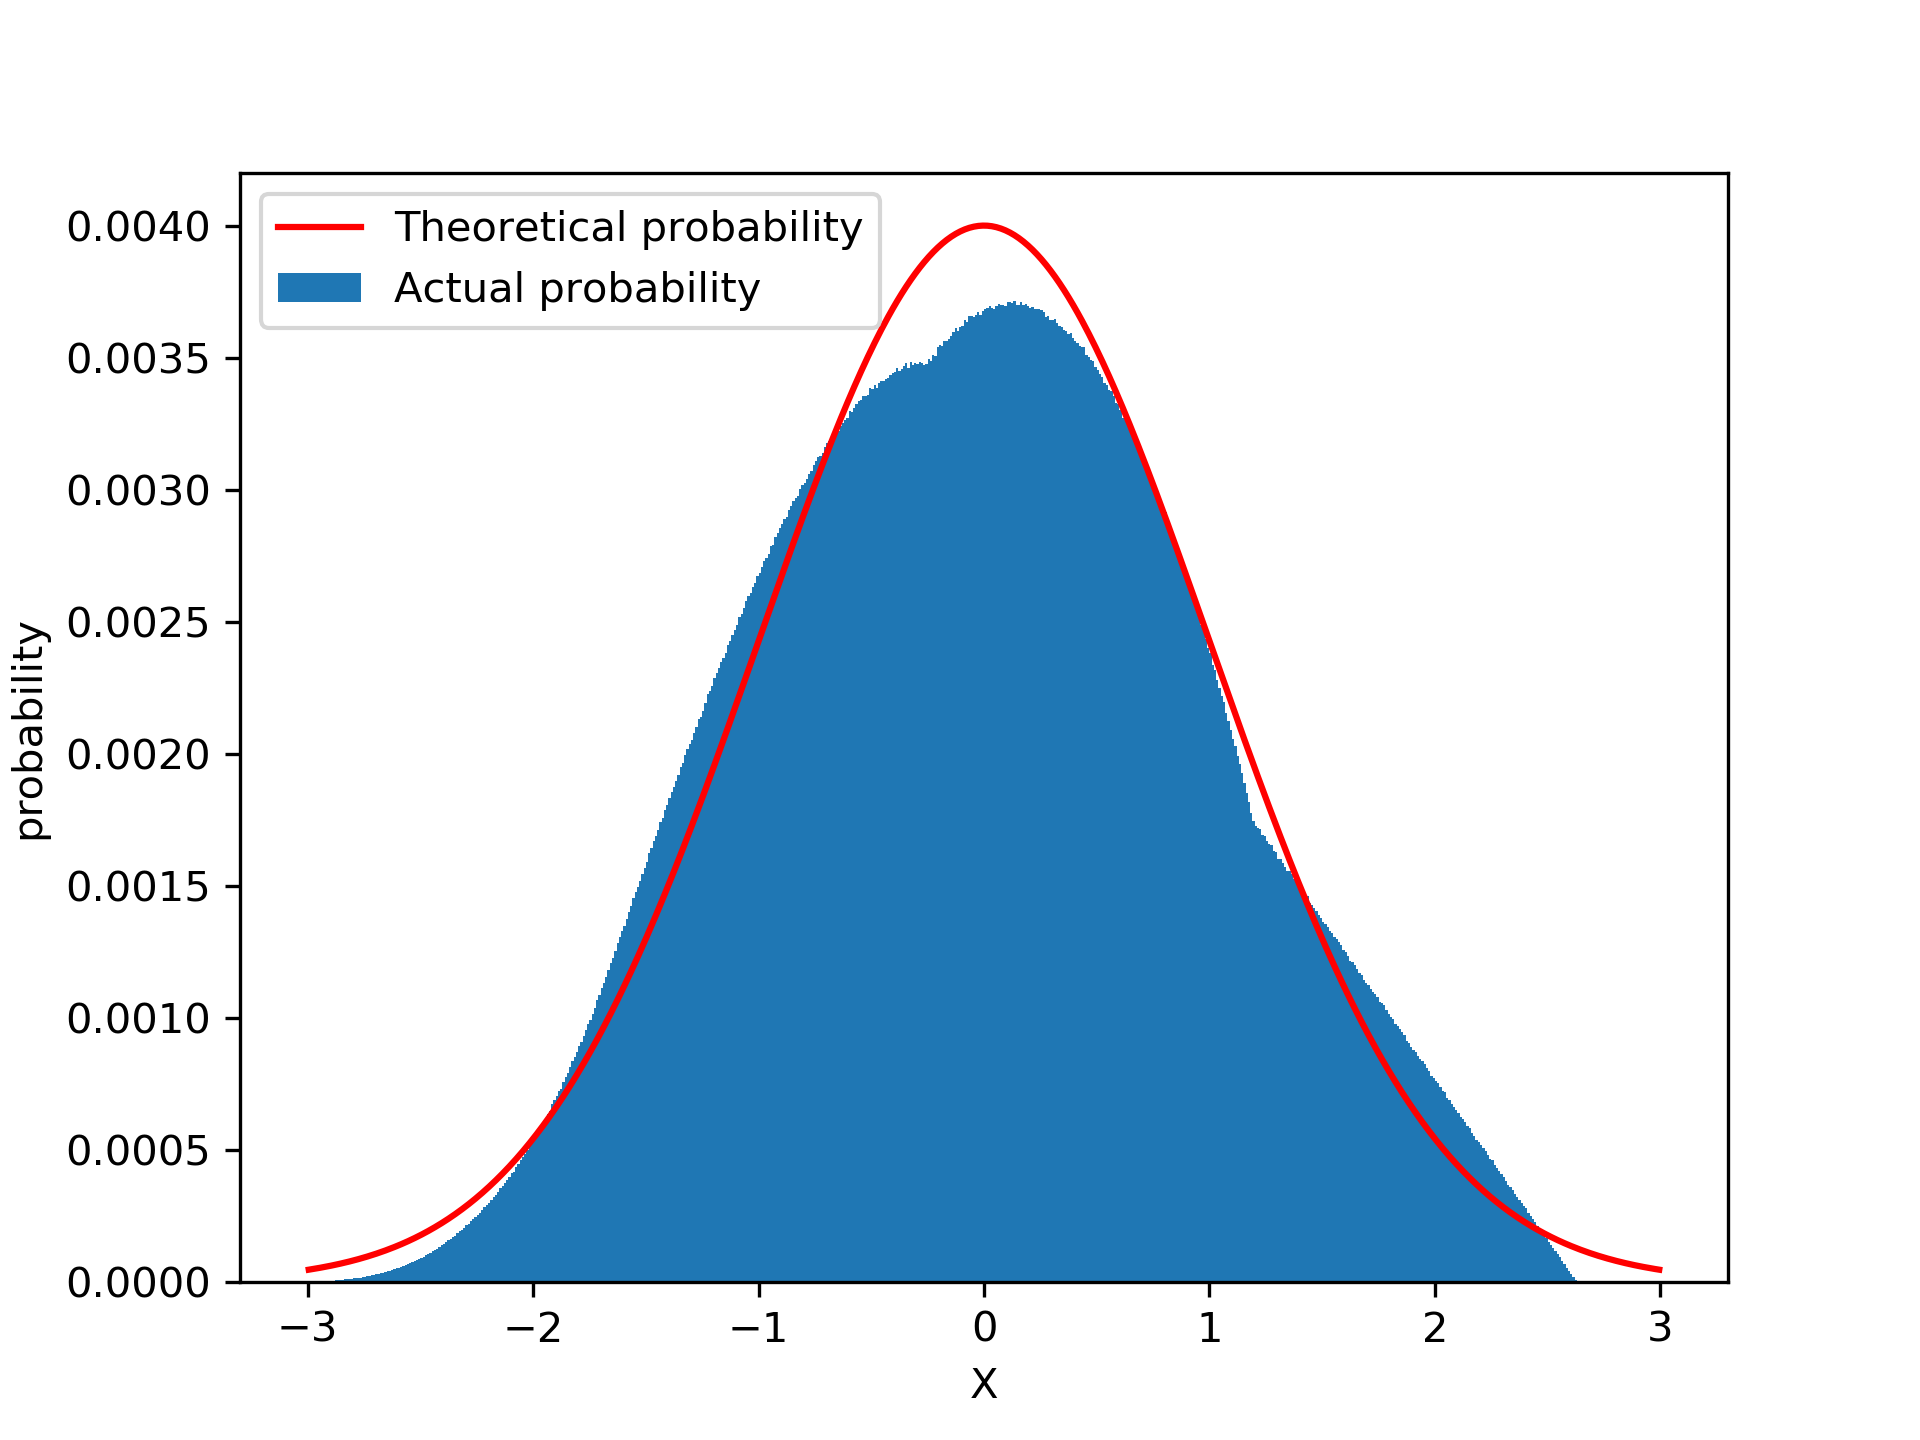
\includegraphics[width=4cm] {3-8-2.png}
}
\subfigure[每次抽样5个点]{
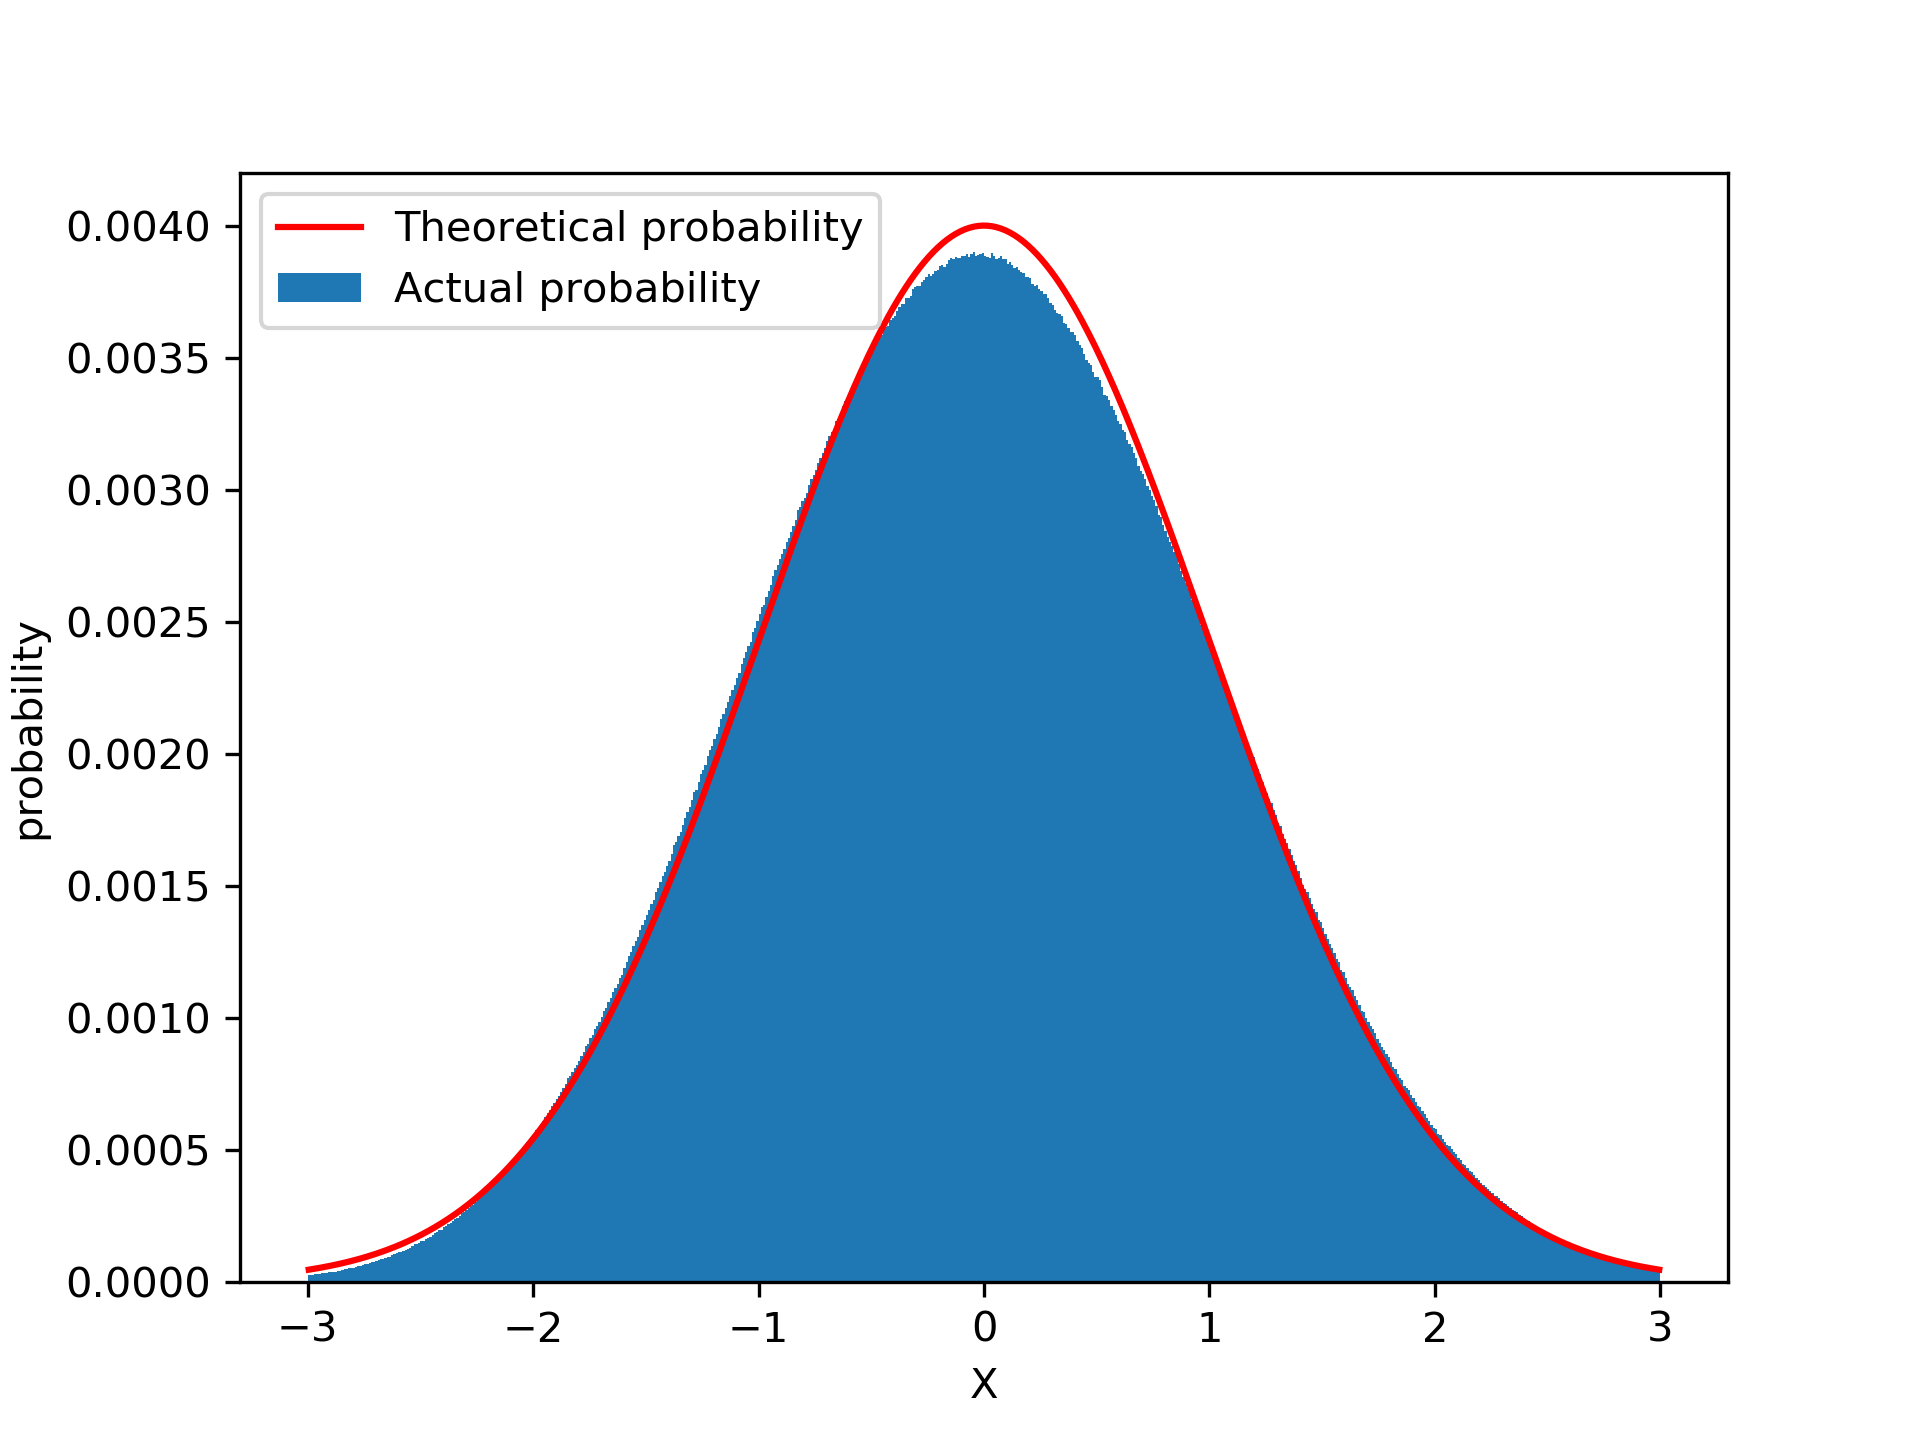
\includegraphics[width=4cm] {3-8-5.png}
}      
\subfigure[每次抽样10个点]{
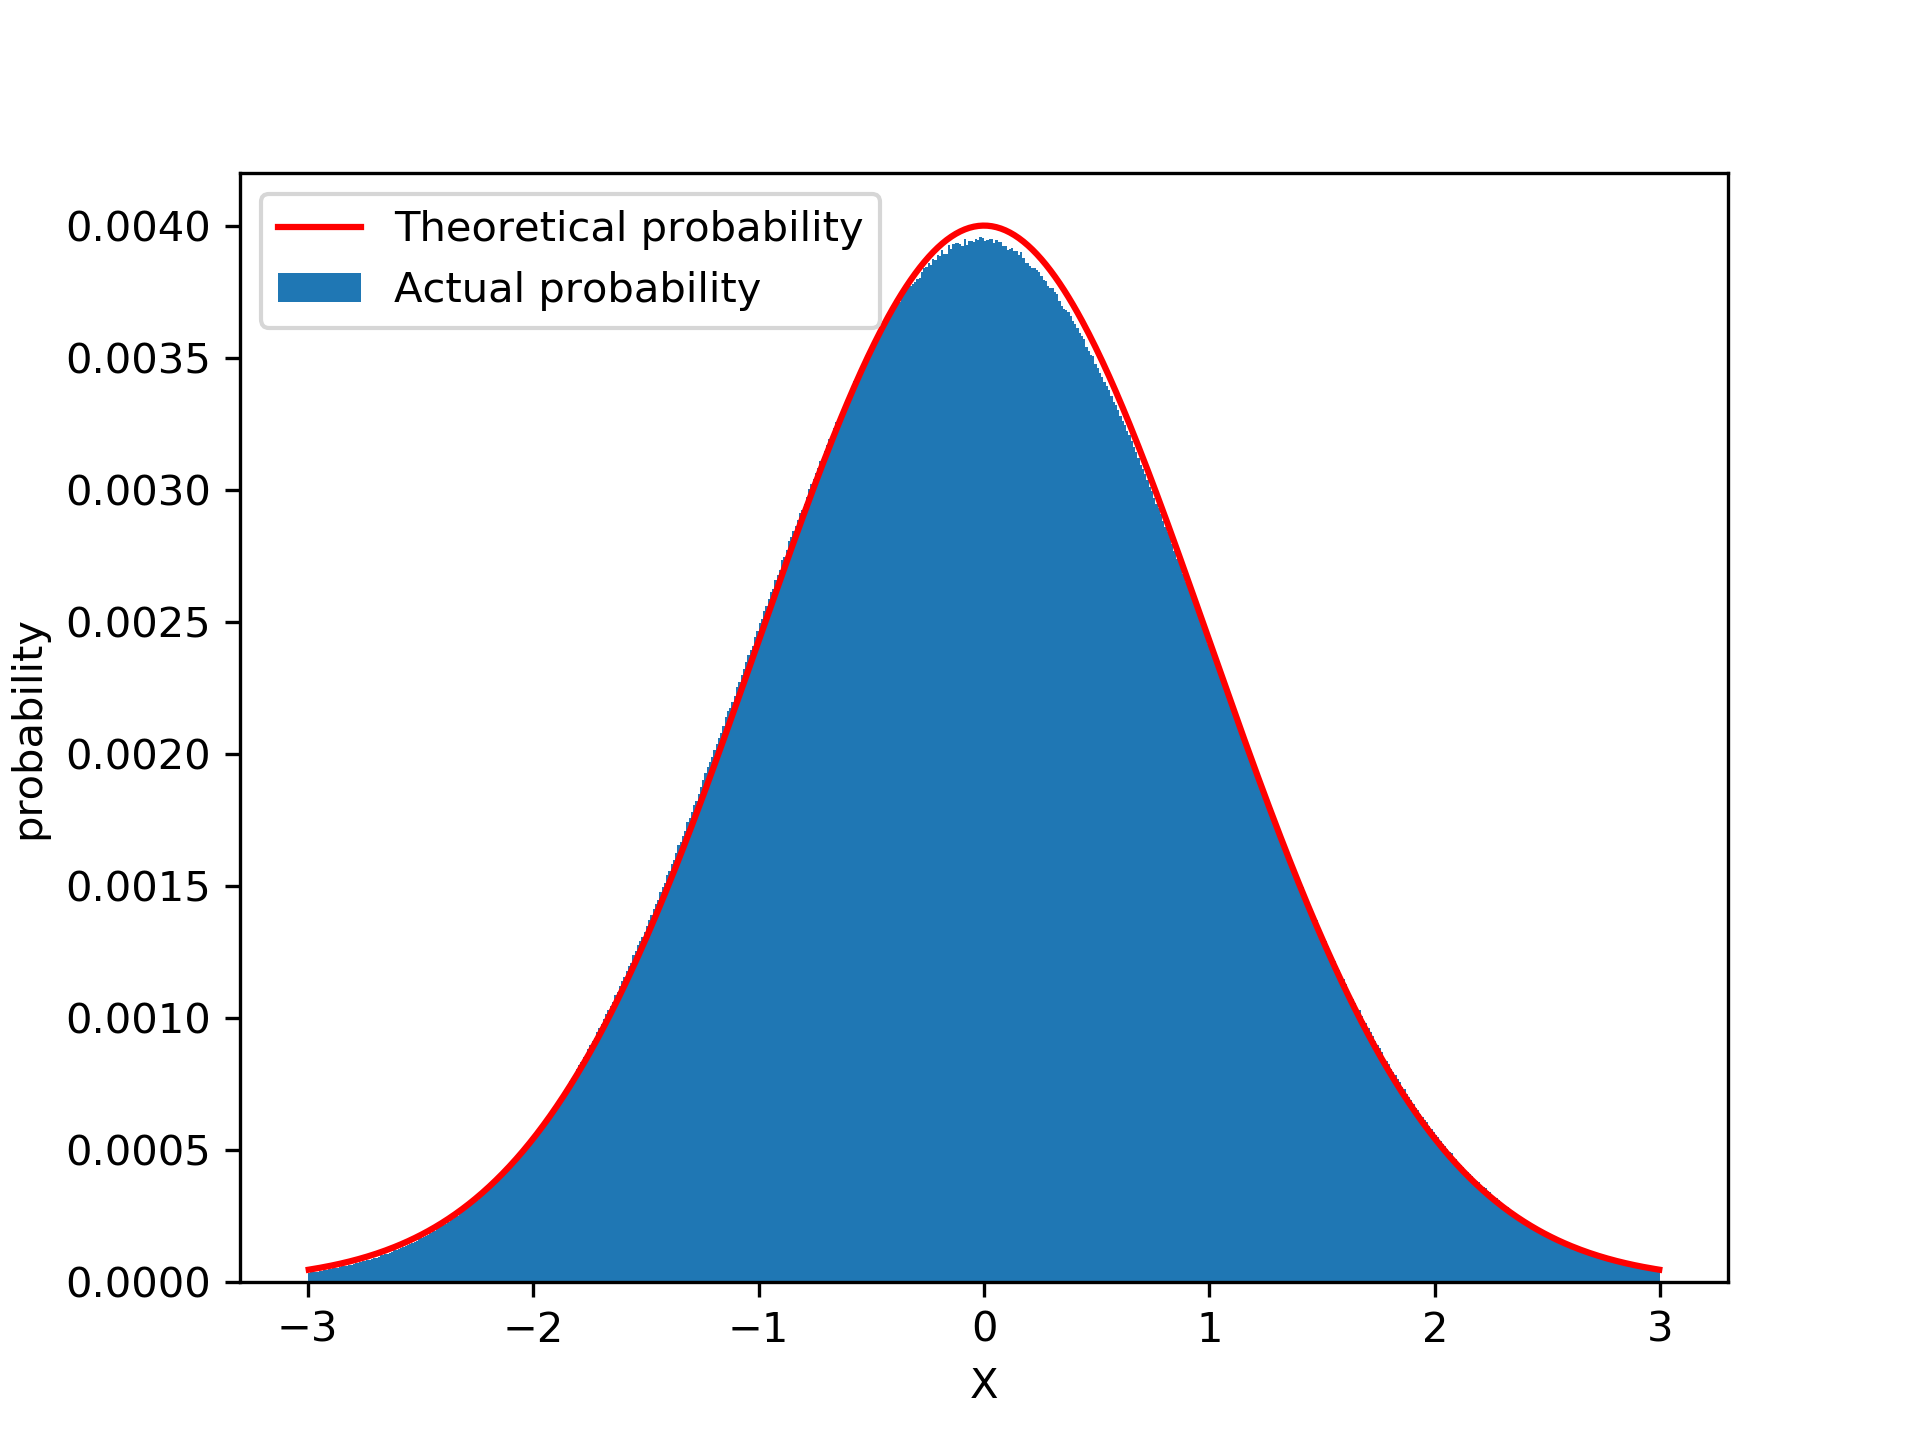
\includegraphics[width=4cm] {3-8-10.png}
}      
\caption{3号分布计算$10^{8}$次后的结果}      
\end{figure}



\newpage
 可以看出对于3号分布随着计算计算次数和每次抽样个数的增加,其统计量的分布与标准正态分布越来越接近。
 
 通过对此3个分布的计算结果,看出每次抽样个数越多时,统计量的概率分布越接近于标准正态分布,中心极限定理得到了验证。
 

\section{心得与体会}
通过此次作业,对中心极限定理有了更深刻的认识。

通过编程作业,也更加熟悉了一些C语言和\LaTeX 。

\newpage
\section{附录}

\begin{appendices}


\section{C语言源程序}
\begin{lstlisting}[language = C]
#include <stdio.h>
#include <stdlib.h>
#include <time.h>
#include <math.h>
#define a 16807
#define b 0
#define m 2147483647
#define r (m%a)
#define q (m/a)
#define Pi 3.1415926
#define k 600
#define GETMATELEM(base,i,j,imax) ((*(base + i * imax + j))) //取二维数组元素



int my_filewriter_double(char str[],double num[],int n){
    FILE * fp;
    fp = fopen(str,"w+");

    for(int i=0;i<(n-1);i++)
    {
        fprintf(fp,"%lf,",num[i]);

    }
    fprintf(fp,"%lf",num[n-1]);    //最后一个数据后不加 ","
    fclose(fp);
    return 0;
}




// Schrage 方法产生随机数
int my_schrage(int seed){
    int x;
    if(seed == m-1){
        if(a >=  b){    //由于Schrage方法只对z in (0,m-1)成立,故这里要讨论z == m-1的情况
            x = m + (b-a) % m;
        }
        else   x =  (b-a) % m;

    }
    else x = ((a * (seed % q) - r * (seed /  q)) + b % m ) % m;  //递推式
    return x;
}


int my_function1(double p[],int N,int n){
    double beta; //存放统计量计算结果
    int x = 1; //16807方法递推数列,初始种子值为1
    double y;  //y为(0,1)均匀抽取的点
    int flag = 0;
    for(int i = 0;i<k;i++){  //概率分布数组初始化
        p[i] = 0;
    }
    for(;flag<N;){  //控制计算次数
        beta = 0;
        for(int i = 0;i<n;i++){  //控制每次计算时抽取的点数
            x = my_schrage(x);   //随机数递推数列
            if(x >= 0) y = (double)x/m;
            else y = (double)(x+m)/m;  //y为(0,1)均匀抽取的点
            if(y <= 0.5){
                beta += (sqrt(2*y)-1)/n;
            }
            else beta += (1-sqrt(2-2*y))/n;  //直接抽样法并计算得到第i次抽样结果的平均值
        }
        beta = beta*sqrt(6*n);  //计算统计量
        
        if(beta <= 3 && beta >= -3){   //统计统计量分布
            p[(int) floor( (beta+3)/6*k) ] += (double)1/N  ;
            flag++;
        }
    }
    return 0;
}

int my_function2(double p[],int N,int n){
    double beta; //存放统计量计算结果
        int x = 1; //16807方法递推数列,初始种子值为1
        double y;  //y为(0,1)均匀抽取的点
        int flag = 0;
        for(int i = 0;i<k;i++){  //概率分布数组初始化
            p[i] = 0;
        }
        for(;flag<N;){  //控制计算次数
            beta = 0;
            for(int i = 0;i<n;i++){  //控制每次计算时抽取的点数
                x = my_schrage(x);   //随机数递推数列
                if(x >= 0) y = (double)x/m;
                else y = (double)(x+m)/m;   //y为(0,1)均匀抽取的点
                beta += (y+1)/n;    //直接抽样法并计算得到第i次抽样结果的平均值
            }
            beta = (beta-1.5)*sqrt(12*n);   //计算统计量
            if(beta <= 3 && beta >= -3){  //统计统计量分布
                p[(int) floor( (beta+3)/6*k) ] += (double)1/N  ;
                flag++;
            }
        }
        return 0;
}



int my_function3(double p[],int N,int n){
    double beta; //存放统计量计算结果
    int x = 1; //16807方法递推数列,初始种子值为1
    double y;  //y为(0,1)均匀抽取的点
    int flag = 0;
    for(int i = 0;i<k;i++){   //概率分布数组初始化
        p[i] = 0;
    }
    for(;flag<N;){   //控制计算次数
        beta = 0;
        for(int i = 0;i<n;i++){  //控制每次计算时抽取的点数
            x = my_schrage(x);   //随机数递推数列
            if(x >= 0) y = (double)x/m;
            else y = (double)(x+m)/m;   //y为(0,1)均匀抽取的点
            if(y <= 0.5){    //直接抽样法并计算得到第i次抽样结果的平均值
                beta += (sqrt(2*y)-1)/n;
            }
            else beta += (2*y-1)/n;
        }
        beta = 12*(beta-(double)1/12)*sqrt(n)/sqrt(35);   //计算统计量
        
        if(beta <= 3 && beta >= -3){   //统计统计量分布
            p[(int) floor( (beta+3)/6*k) ] += (double)1/N  ;
            flag++;
        }
    }
    return 0;
}



int main(int argc, const char * argv[]) {
    int N;    //总计算次数
    int n;   //每此计算所选点数
    double p1[k];
    double p2[k];
    double p3[k];
    char str[50];
    printf("请输入您所需的计算次数:");
    while (!scanf("%d",&N)){   //简单的输入检查
        gets(str);
        printf("\nInput error,please try again\n");
        printf("请输入您所需的计算次数:");
    }
    
    printf("请输入您每次计算所用的点数:");
    while (!scanf("%d",&n)){   //简单的输入检查
        gets(str);
        printf("\nInput error,please try again\n");
        printf("请输入您每次计算所用的点数:");
    }

    if(N*n >1000000) printf("您输入的参数已接受,正在计算请稍等片刻~\n");
    
    my_function1(p1,N,n);
    my_function2(p2, N, n);
    my_function3(p3, N, n);
    
    my_filewriter_double("function1.txt", p1, k);
    my_filewriter_double("function2.txt", p2, k);
    my_filewriter_double("function3.txt", p3, k);
    
    return 0;
}

\end{lstlisting}

\newpage

\section{可视化绘图python程序源码}

\begin{lstlisting}[language = python]

import matplotlib.pyplot as plt
from mpl_toolkits.mplot3d import Axes3D
import numpy as np
#from IPython.core.pylabtools import figsize # import figsize
#figsize(12.5, 4) # 设置 figsize
plt.rcParams['savefig.dpi'] = 300 #图片像素
plt.rcParams['figure.dpi'] = 300 #分辨率
# 默认的像素:[6.0,4.0],分辨率为100,图片尺寸为 600&400
fig = plt.figure()
ax1 = fig.add_subplot(111)
X = []
Y = []

with open('problem 9/3-8-10.txt', 'r') as f:
    while True:
        lines = f.readline() # 整行读取数据
        if not lines:
            break
        Y = [float(i) for i in lines.split(',')]  # 将整行数据分割处理
    Y = np.array(Y) # 将数据从list类型转换为array类型。


X = np.arange(-2.995, 3.005, 0.01)

plt.bar(x=X, height=Y, width=0.01, label='Actual probability')
ax1.legend(loc=1)
ax1.set_ylabel('probability')
#plt.savefig("1.png")


oY = np.exp(-X**2/2)*0.01/2.499860889


ax1.plot(X, oY, 'r', label='Theoretical probability')
ax1.legend(loc=2)
#plt.ylim([0,0.0055])
plt.xlabel('X')


plt.savefig("2.png")


\end{lstlisting}


\end{appendices}




\end{document}
